\documentclass[a4paper,10pt]{report}

\usepackage{tikz}
\usetikzlibrary{shadows.blur}
\usetikzlibrary{shapes.symbols}

\usepackage{fancybox, graphicx}
\usepackage{hyperref}
\usepackage{amsmath}
\usepackage{amssymb}
\usepackage{xspace}
\pagestyle{headings}
\usepackage[total={6.5in,10.0in}, top=1in, left=.8in, includefoot]{geometry}
\usepackage{float}
\restylefloat{table}
\usepackage{listings}
\usepackage{color}
\definecolor{red}{rgb}{1,0,0}
\definecolor{gray}{rgb}{0.4,0.4,0.4}
\definecolor{darkblue}{rgb}{0.0,0.0,0.58}
\definecolor{attributeColor}{rgb}{0.96,0.517,0.29}
\definecolor{darkgreen}{rgb}{0,.392,0}
\definecolor{stringColor}{rgb}{0.6,0.2,0}
\usepackage{array,multirow}
\usepackage{longtable}
\LTcapwidth=\textwidth
\usepackage{cleveref}
\usepackage{bbding}
\crefname{section}{�}{��}
\Crefname{section}{�}{��}
\usepackage[utf8]{inputenc}
\usepackage{tablefootnote}
\usepackage{algorithmicx}
\usepackage[modulo, pagewise]{lineno}
\nolinenumbers
\usepackage{fancyhdr}
\pagestyle{fancy}
\fancyhead[RO]{PharmML 0.8}
\fancyhead[RE]{\itshape\nouppercase{\leftmark}}
\usepackage{booktabs}
\usepackage{fixltx2e}
\usepackage{array,arydshln}
\usepackage{wrapfig}
\usepackage{makeidx}
\usepackage{varwidth}
\usepackage{lipsum}
\usepackage{blkarray}

\usepackage{makecell}
\usepackage{multicol}
\usepackage{url}
\usepackage{verbatimbox}
\usepackage{xcolor}
\usepackage{cancel}
\usepackage{algpseudocode}

\setlength{\tabcolsep}{5pt}

\usepackage{caption} 
\captionsetup[table]{skip=5pt}
\captionsetup[longtable]{skip=5pt}
\captionsetup[figure]{skip=1pt}

\def\bmp{\begin{minipage}{0.48\linewidth}\small} 
\def\emp{\end{minipage}\smallskip}

\setlength\dashlinedash{0.4pt}
\setlength\dashlinegap{1pt}
\setlength\arrayrulewidth{0.5pt}

\hypersetup{pageanchor=false}

\newcommand{\myStartLine}{\par
  \kern8pt % space above the rules
  \hrule height 0.5pt
  \kern3pt % space below the rules
}
\newcommand{\myEndLine}{\par
  \kern3pt % space above the rules
  \hrule height 1.5pt
  \kern12pt % space below the rules
}

% Colours stolen from SBML pkg spec class
\definecolor{lightblue}{rgb}{0.07, 0.50, 0.78}
\definecolor{mediumgreen}{rgb}{0.1, 0.6, 0.3}

\definecolor{hellgelb}{rgb}{1,1,0.9}
\definecolor{colKeys}{rgb}{0,0,1}
\definecolor{colIdentifier}{rgb}{0,0,0}
\definecolor{colComments}{rgb}{1,0,0}
\definecolor{colString}{rgb}{0,0.5,0}

\lstset{
  basicstyle=\ttfamily,
  columns=fullflexible,
  showstringspaces=false,
  commentstyle=\color{gray}\upshape
%  numbers=left,
%  stepnumber=5
}

\newcommand{\HRule}{\rule{\linewidth}{0.5mm}}

\lstdefinelanguage{XML}
{
  basicstyle=\ttfamily\footnotesize,
  morestring=[b]",
  morestring=[s]{>}{<},
  moredelim=[s][\bfseries\color{darkblue}]{<}{\ },
  moredelim=[s][\bfseries\color{darkblue}]{</}{>},
  moredelim=[l][\bfseries\color{darkblue}]{/>},
  moredelim=[l][\bfseries\color{darkblue}]{>},
  morecomment=[s]{<?}{?>},
  morecomment=[s]{<![CDATA[}{]]>},
  moredelim=[s][\bfseries\color{darkgreen}]{<!--}{-->},
  commentstyle=\color{darkgreen},
  stringstyle=\color{stringColor},
  identifierstyle=\color{red},
  keywordstyle=\color{attributeColor},
  morekeywords={oid,columnId,columnIdRef,symbId,symbolType,op,columnNum,columnType,
  valueType,inputTarget,blkId,blkIdRef,symbIdRef,xmlns,version,type,VariableMapping,
  IndividualMapping,schemaLocation,xs,xsi,NONMEMdataSet,matrixType,opType,order,
  math,ct,ds,mdef,mstep,mml,un,name,definition,writtenVersion,id,inputType,oidRef,catId,
  length,default,vectorIndex,diagDefault,offDiagDefault,row,column,numbRows,numbCols,
  dataSymbol,modelSymbol,ordered,compartmentNo,compNo,ordered,linkFunction,varId,
  censoringType,dataSymbol,modelSymbol,MarkovOrder,deviationMatrixType,implementedBy,
  argument,admNumber,transformId,transformIdRef,catIdRef,headerType,rowNumber,
  toolName,dataCode,missingDataType,regressor,fixed,transformation,transform,symbol} % list your attributes here
}

\lstdefinelanguage{MLX} 
{
  basicstyle=\ttfamily\small,
  morestring=[b]",
  morestring=[s]{>}{<},
  moredelim=[s][\bfseries\color{darkblue}]{<}{\ },
  moredelim=[s][\bfseries\color{darkblue}]{</}{>},
  moredelim=[l][\bfseries\color{darkblue}]{/>},
  moredelim=[l][\bfseries\color{darkblue}]{>},
  morecomment=[s]{<?}{?>},
  morecomment=[s]{<!--}{-->},
  morecomment=[s]{<![CDATA[}{]]>},
  commentstyle=\color{darkgreen},
  stringstyle=\color{stringColor},
  identifierstyle=\color{black},
  keywordstyle=\color{attributeColor},
  morekeywords={dads} % list your attributes here
}

\lstdefinelanguage{NM}
{
  basicstyle=\sffamily\small,
  morestring=[b]",
  morestring=[s]{>}{<},
  moredelim=[is][\bfseries\color{red}]{[*}{*]},
  moredelim=[s][\bfseries\color{darkblue}]{<}{\ },
  moredelim=[s][\bfseries\color{darkblue}]{</}{>},
  moredelim=[l][\bfseries\color{darkblue}]{/>},
  moredelim=[l][\bfseries\color{darkblue}]{>},
  morecomment=[s]{<?}{?>},
  morecomment=[s]{<!--}{-->},
  morecomment=[s]{<![CDATA[}{]]>},
  commentstyle=\color{darkgreen},
  stringstyle=\color{stringColor},
  identifierstyle=\color{black},
  keywordstyle=\color{attributeColor},
  morekeywords={kjkj} % list your attributes here
}

\newcommand{\cellml}{CellML\xspace}
\newcommand{\sbml}{SBML\xspace}
\newcommand{\sedml}{SED-ML\xspace}
\newcommand{\mathml}{MathML\xspace}
\newcommand{\uncertml}{UncertML\xspace}
\newcommand{\pml}{PharmML\xspace}
\newcommand{\pharmml}{PharmML\xspace}
\newcommand{\xelem}[1]{\texttt{<#1>}\index{XML Element!\texttt{<#1>}}}
\newcommand{\xatt}[1]{\texttt{#1}\index{XML Attribute!\texttt{#1}}}
\newcommand{\var}[1]{\ensuremath{\mathit{#1}}\index{Symbol!\ensuremath{\mathit{#1}}}}
\newcommand{\dscol}[1]{\texttt{#1}}
\newcommand{\attval}[1]{``\texttt{#1}''}

%Counter for examples chap
\newcounter{examples}
\newcommand{\eglabel}[1]{\refstepcounter{examples}\label{egsec:#1}}
\newcommand{\egref}[1]{\ref{egsec:#1}}

\setcounter{secnumdepth}{3}
\setcounter{tocdepth}{3}

\begin{document}

\begin{titlepage}
\begin{center}

% Upper part of the page. The '~' is needed because \\
% only works if a paragraph has started.

\includegraphics[width=0.35\textwidth]{./logo/ddmore_logo}~\\[1cm]

%\textsc{\LARGE }\\[1.5cm]
%
\textsc{\Large Internal Release}\\[0.5cm]

% Title
\HRule \\[0.4cm]
{ \huge \bfseries Extensions in PharmML 0.8 \\[0.4cm] }

\HRule \\[1.5cm]

% Author and supervisor
\begin{minipage}{0.5\textwidth}
\begin{flushleft} \large
\emph{Authors:}\\
Maciej J \textsc{Swat}\\
Florent \textsc{Yvon}\\
Sarala \textsc{Wimalaratne}\\
\end{flushleft}
\end{minipage}
\begin{minipage}{0.4\textwidth}
\begin{flushright} \large
\emph{with contributions from:} \\
Roberto \textsc{Bizzotto} \\
Gareth \textsc{Smith} \\
\end{flushright}
\end{minipage}

\vfill
\begin{figure}[htb]
\centering
  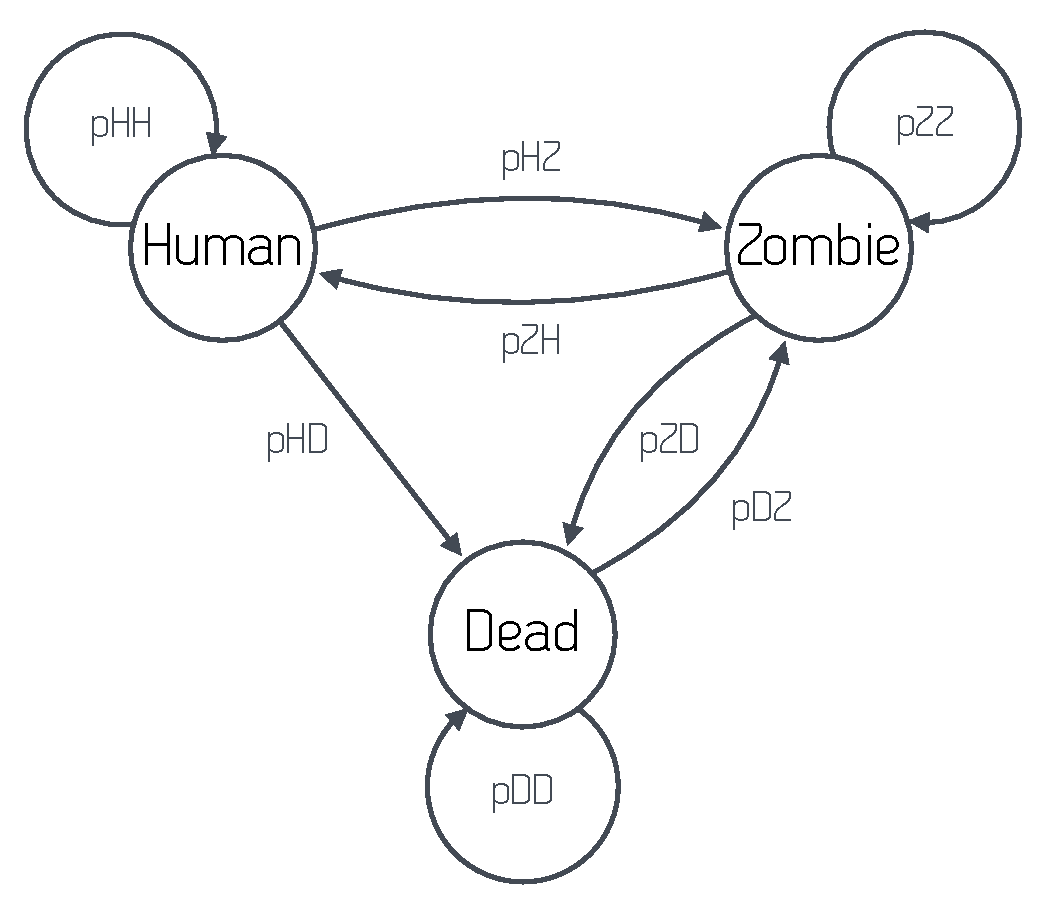
\includegraphics[width=90mm]{pics/MarkovZombie_title}
\end{figure}



\vfill

% Bottom of the page
{\large \today \\}

\end{center}
\end{titlepage} 

\linenumbers
\tableofcontents


%%%%%%%%%%%%%%%%%%%%%%%%%%%%%%%%%%%%%%%%%%%%%%%%%%%%%%%%%%%%%%%%%%%%%%
%%%%%%%%%%%%%%%%%%%%%%%%%%%%%%%%%%%%%%%%%%%%%%%%%%%%%%%%%%%%%%%%%%%%%%%
%%%%%%%%%%%%%%%%%%%%%%%%%%%%%%%%%%%%%%%%%%%%%%%%%%%%%%%%%%%%%%%%%%%%%%%
%%%%%%%%%%%%%%%%%%%%%%%%%%%%%%%%%%%%%%%%%%%%%%%%%%%%%%%%%%%%%%%%%%%%%%%
\chapter{Overview}

This document describes extensions and changes in \pml compared to version 0.7.3
released in September 2015. The changes so far are visualised in Figure \ref{fig:history}.

\begin{figure}[ht!]
\centering
  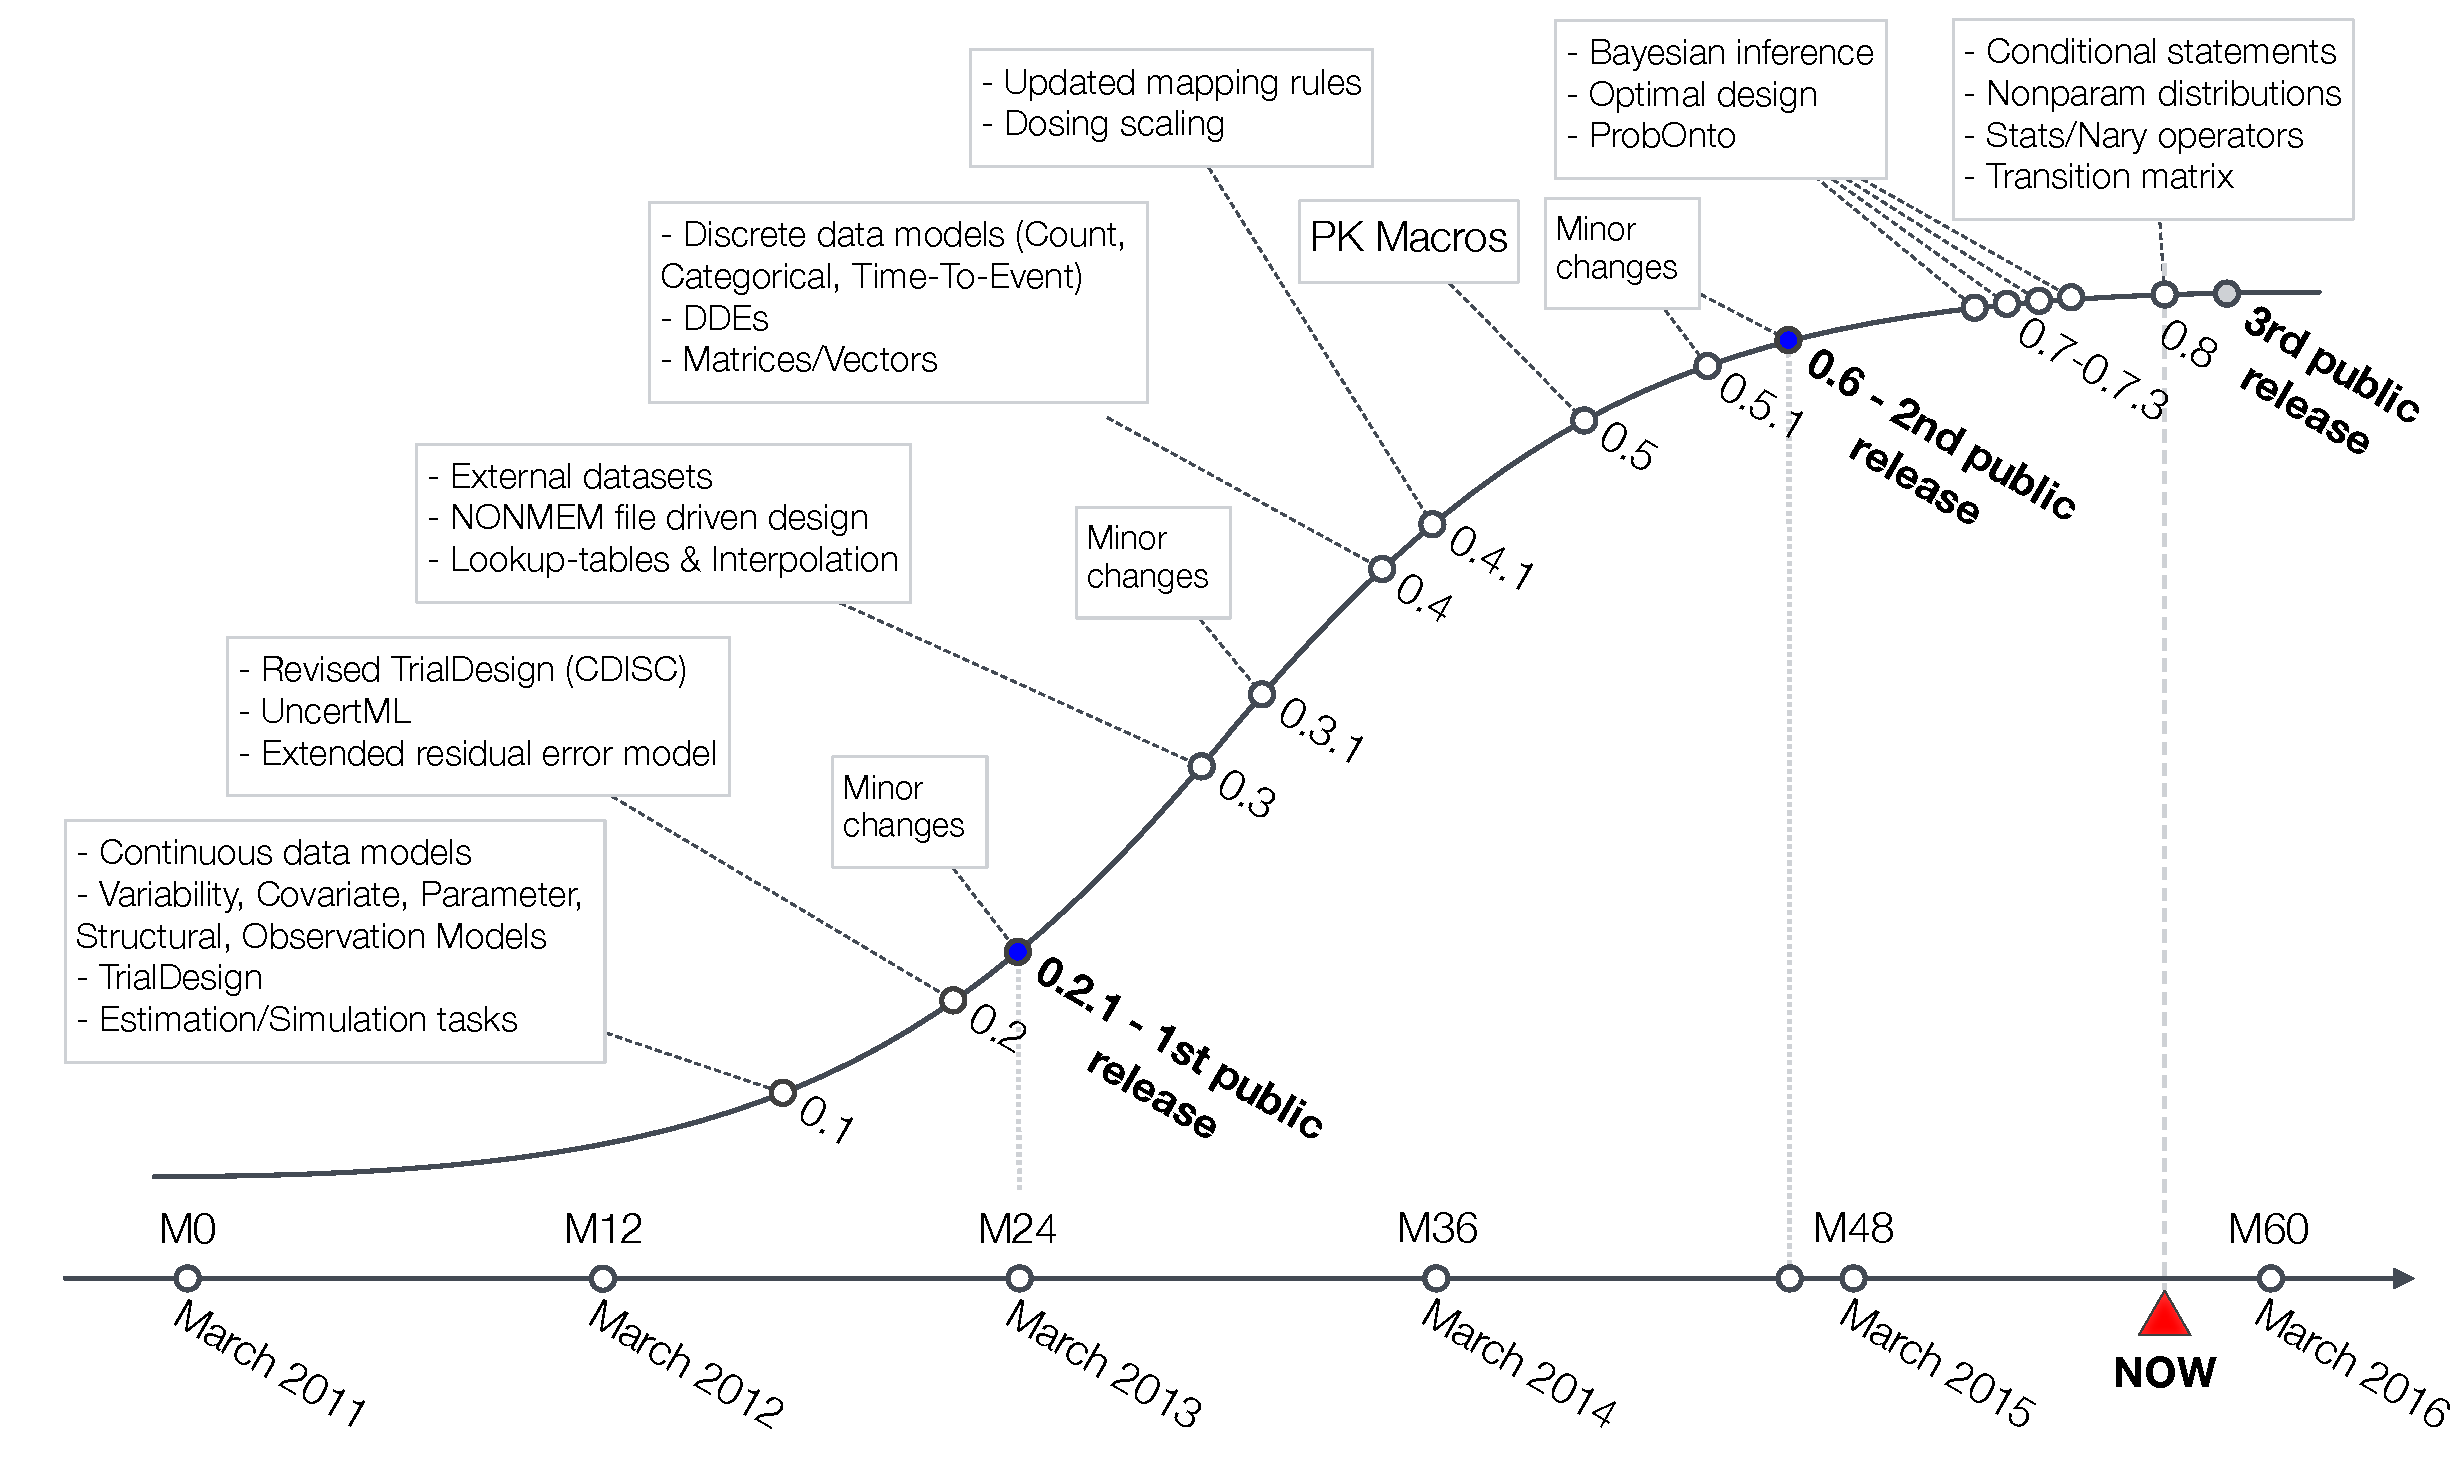
\includegraphics[width=160mm]{pics/Timeline08.pdf}
 \caption{Release history.}
 \label{fig:history}
\end{figure}

\section*{Major changes/extensions in version 0.8}
The following table summarises the major changes described in detail in following chapters. 
\marginpar{FINISH \\FINISH \\FINISH}

\captionsetup[longtable]{skip=1em}
\LTcapwidth=\textwidth
\begin{center}
%\renewcommand{\arraystretch}{1.1}%
\begin{longtable}{lll}
\hline
\hline
\pml element 				&  version $\le$ 0.7.3 	& version 0.8 \\
or modelling aspect 			& 					& \\
%\hline
%\hline
%  \multicolumn{3}{c}{\textit{Model Definition}}		\\
%\hline
\hline
Assignment statements		& not supported		& {\color{red} \scshape{new}} \xelem{AssignStatement} element available \\
Section \ref{sec:assignments}	& 					& in covariate, parameter, structural and \\
						&					& observation models \\
\hline
Conditional statements		& not supported		& {\color{red} \scshape{new}} \xelem{ConditionalStatement} element with \\
Section \ref{sec:conditionalStatements} &				& child elements \xelem{If}, \xelem{ElseIf} and \xelem{Else} \\
\hline
Nested piecewise			& not supported		& supported \\
Section \ref{sec:nestedPiecewise}	&				& \\
\hline
Probability functions			& not supported		& {\color{red} \scshape{new}} \xelem{PDF}, \xelem{CDF}, \xelem{HF}, \xelem{SF} elements \\
Section \ref{sec:probabFunctions}	&				& for every continuous distribution available in \\
						&					& ProbOnto \\
\hline
Time-to-event data models	& explicit hazard/survival	& encodable using \xelem{HF}/\xelem{SF} (see above)\\
Section \ref{subsec:TTEmodel} & formulas required	& \\
\hline
Nonparametric distribution	& not supported		&  accessible via ProbOnto with {\color{red} \scshape{new}} \\ 
Section \ref{sec:nonParamDistribs}	& 				& \xatt{RandomSample}, \xatt{SystematicSample}	\\
						&					& \xatt{UnknownSample} and \xatt{weight} parameter \\
\hline
Random realisations			& not supported		& available now in ProbOnto \\
Section \ref{sec:randRealisations}	 &				& as \xelem{Realisation} {\color{red} \scshape{new}} \\
\hline
Markov models				& only pair-wise transition	& {\color{red} \scshape{new}} \xelem{TransitionMatrix} element with  \\
Section \ref{sec:MM}		& probabilities			& \xatt{type} attribute: \emph{leftStochastic}, \emph{rightStochastic} \\
						&  					& and \emph{doublyStochastic} \\
\hline
N-ary operators			& not supported		& {\color{red} \scshape{new}} \xatt{plus}, \xatt{times}, \xatt{min}, \xatt{max}, \xatt{gcd}, \xatt{lcm}\\
Section \ref{sec:NaryOps}	&					& \\
\hline
Statistical operators			& not supported		& {\color{red} \scshape{new}} \xatt{centredMoment}, \xatt{coefficientOfVariation},\\
Section \ref{sec:statsOps}	&					& \xatt{correlation}, \xatt{decile}, \xatt{geometricMean}, \xatt{kurtosis}, \\
						&					& \xatt{mean}, \xatt{median}, \xatt{mode}, \xatt{moment}, \xatt{percentile}, \xatt{quantile} \\
						&					& \xatt{quartile}, \xatt{range}, \xatt{skewness}, \xatt{standardDeviation}, \\
						&					& \xatt{variance}\\
\hline
Covariate model			& covariate type not 		& {\color{red} \scshape{new}} attribute \xatt{type} with values \\	
Section \ref{sec:covVsRegs}	& annotated			& \emph{occasionDependent}, \emph{timeDependent}, \\
						&					& \emph{constant}\\
Categorical covariate model	& defining distribution only & -- full distribution support via ProbOnto \\
Section \ref{sec:catCovModel}	& with \xelem{Probability}	& \\
						& element				& \\
						& 				 	& -- covariates declaration/assignment \\
						& 					& -- conditional distributions allowed \\
\hline
Dataset  					& single ignore character	& conditional ignoring statements supported \\
						& declaration only		&  \\
\hline
\caption{Overview of major differences between versions 0.8 and 0.7.3}
\label{figTable:overviewTable}
\vspace{-2em}
\end{longtable}
\end{center}



%%%%%%%%%%%%%%%%%%%%%%%%%%%%%%%%%%%%%%%%%%%%%%%%%%%%%%%%%%%%%%%%%%%

\chapter{Changes in 0.8}
\label{ch:08changes}

\section{Backwards compatibility with 0.7.3}
The 0.8 version is backwards compatible with 0.7.3 as tested on 
\begin{itemize}
\item 
more then 80 examples provided with each release and
\item 
new 14 IOG use cases\footnote{\url{http://sourceforge.net/projects/ddmore/files/install/SEE/Demonstrator-1.2.0/resources/converter-systemtest-1.3.0-results.zip/download}} publicly released with the Product 4.1.
\end{itemize}
This means that no elements/attributes have been removed, 
renamed or otherwise modified in a way which would make 0.7.3 models 
invalid with respect to the new schema and specification.

\section{Assignment statements}
\label{sec:assignments}

So far assignments were performed together with declarations. 
The new \xelem{AssignStatement} element allows to loosen up this structure and 
do it more flexibly separately. 
For example the following snippet shows how to define a parameter, 
$k$, and subsequently how to assign an expression, $CL/V$, to it.
\begin{longtable}{cc}
\hline
\hline
option supported so far & new option in version 0.8 \\
\hline
\lstset{language=XML}
\begin{lstlisting}
    <!-- declaration & assignment -->
    <IndividualParameter symbId="k">
        <ct:Assign>
            <math:Binop op="divide">
                <ct:SymbRef symbIdRef="CL"/>
                <ct:SymbRef symbIdRef="V"/>
            </math:Binop>
        </ct:Assign>
    </IndividualParameter>
\end{lstlisting}
&
\lstset{language=XML}
\begin{lstlisting}
    <!-- declaration -->
    <IndividualParameter symbId="k"/>
    
    <!-- assignment, k=CL/V -->
    <ct:AssignStatement op="eq">
        <!-- LHS -->
        <ct:SymbRef symbIdRef="k"/>
        <!-- RHS -->
        <math:Binop op="divide">
            <ct:SymbRef symbIdRef="CL"/>
            <ct:SymbRef symbIdRef="V"/>
        </math:Binop>
    </ct:AssignStatement>
\end{lstlisting}
\\
\hline
\caption{Assignment statements are new in v0.8.}
\label{tab:comparisonAssignments}
\vspace{-1em}
\end{longtable}%
The assignment element is available in the covariate, parameter, structural 
and the observation models. It can be applied generally but will turn out to be 
especially useful in connection with the new conditional assignment 
statements, see section \ref{sec:conditionalStatements}.

\subsection{Assignment rules}
\begin{itemize}
\item 
One assignment per \xelem{AssignStatement} is allowed.
\item
Left and right hand sides of the assignment can be any expressions 
which evaluate to scalar values.
\item 
Parameters and variables used within the assignment statements
must the declared before, see for an example Table \ref{tab:comparisonAssignments} (right).
\item 
Only one assignment of each parameter or variable is allowed within a model, 
unless used in a conditional statement, see section \ref{subset:rulesCS}.
\end{itemize}

\subsection{New opportunities}
\label{subsec:greco}
The introduction of assignment statements opens few new opportunities 
to encode models relevant for studying of drug-drug interaction models.
While the majority of such models was implementable in previous versions,
the so-called \emph{Greco-model}, \cite{Greco:1990qv}, \cite{kabera2010d},
shown below is treatable in PharmML only thanks to this extension 
\begin{align}
\frac{d_1}{\mu_1 \big[\frac{E}{E_c - E} \big]^{1/m_1}} + \frac{d_2}{\mu_2 \big[\frac{E}{E_c - E} \big]^{1/m_2}} + 
\frac{\alpha\,d_1d_2}{\mu_1 \mu_2 \big[\frac{E}{E_c - E} \big]^{(1/2m_1+1/2m_2)}} = 1
\nonumber
\end{align}
This is a pharmacodynamic model for a combined effect, $E$, a function of two drug 
doses, $d_1$ and $d_2$, which does not have a \emph{closed} form. In other words 
the effect cannot be expressed directly in terms of $d_1$ and $d_2$, i.e. there is no
such function with $E = f(d_1,d_2,\dots)$. The full PharmML code for this model
is provided with this release in the example folder \emph{others}.

It is also for another reason an interesting model. It is one which requires the 
declaration of two independent variables, $d_1$ and $d_2$. Thus the limitation
to only one \xelem{IndependentVariable} has been removed.

\section{Conditional statements}
\label{sec:conditionalStatements}

Conditional assignments are new in this version and provide additional
flexibility to the language. So far only piecewise statement were supported
which have the drawback that only single variables are assigned per statement.

Conditional assignments don't \marginpar{\HandCuffLeft} replace the existing 
piecewise statements, they are an entirely independent structure. 

\subsection{Tool coverage -- capabilities and restrictions}
The extend to which various target tool cover conditional assignments differ
which is an objective issue for the interoperability. Below we summarise
the support and scope of these assignments in the major target tools. 

\begin{itemize}
\item 
\xatt{MLXTRAN}, supports nested conditional \xatt{if-elseif-else-end} statements, e.g.
\lstset{language=MLX}
\begin{lstlisting}
	if (TIME  <=10 && ID == 1)
		G = a1
	elseif (TIME > 10 && ID == 1)
		G = a2
	elseif
		 ...
	end
\end{lstlisting}
%
%	T0=5
%	if t<T0
%		f=A
%	else
%		f= A*exp(-k*(t-T0))
%	end
with following features as listed in the language manual,  \cite{MLXTRANforMonolix:2014}, 
\begin{itemize}
\item 
Several \xatt{elseif} keywords can be chained, and the conditions are 
exclusive in sequence.
\item
A default value can be provided using the keyword \xatt{else}, but also 
as a simple definition preceding the conditional structure
\item
Only intermediate variables can be defined within conditional 
statements, the structure of the model cannot depend on such 
conditions.
\item
The derivatives of an ODE, or the PK elements of a prediction 
sub-model, cannot be defined within conditionals, e.g. the following 
is a valid MLXTRAN code
\lstset{language=MLX}
\begin{lstlisting}
	if t > T_end
		coeff = 0
	else
		coeff = 1
	end
	eta_cond = coeff*eta
	eps_cond = coeff*epsilon
	ddt_TC = s - d*TC - beta*(1-eta_cond)*TC*VL
	ddt_IC = beta*(1-eta_cond)*TC*VL - delta*IC
	ddt_VL = (1-eps_cond)*p*IC - c*VL
\end{lstlisting}
\end{itemize}
\item 
\xatt{NMTRAN}, \cite{NONMEM:2009}, allows nested conditional statements
with the only restriction known to us
\begin{itemize}
\item 
NMTRAN doesn't accept nested conditional statements including 
random variables - described in 'NONMEM Users Guide - Part V', 
page 79, NONMEM 7.2. 
%This relevant discussion will be familiar to you
%\url{https://www.mail-archive.com/nmusers%40globomaxnm.com/msg04626.html}
\end{itemize}
\item 
\xatt{winBUGS}, \cite{Lunn:2009fk}
\begin{itemize}
\item 
supports only a step function of the form
\lstset{language=MLX}
\begin{lstlisting}
		step(e) 1 if e >= 0; 0 otherwise
\end{lstlisting}
where 'e' any expression
\item
Note however, that according to the winBUGS 
translation team, in principle, thanks to the Pascal language interface, almost 
virtually any nested conditional statement can be implemented in WinBUGS. 
%More precisely single assignments are allowed only, see rule 2 in section \ref{subset:rulesCS}. 
\end{itemize}
\item
Common Converter, provided by Gareth Smith (Cyprotex) is able to handle 
(nested) conditional statements. 
\item
\xatt{STAN}, \cite{stan-manual:2015b}, the potential future target tool for the DDmoRe
interoperability platform offers unrestricted support for the conditional statements.
\end{itemize}

\subsection{Definition}
The general form of the (nested) conditional statement looks as follows. 
\bigskip
\begin{algorithmic}
	\If {( condition1 )}
	    \State statement1
	\ElsIf{( condition2 )} 
	    \State statement2
	\ElsIf{( conditionN-1 )} 
	    \State statementN-1
	\Else
	    \State statementN
	\EndIf
\end{algorithmic}
\bigskip
The following definition of the conditional statement have been adapted from the 
STAN specification, \cite{stan-manual:2015b}: \\
There must be a single leading \xatt{if} clause, which may be followed by any number of
\xatt{else if} clauses, all of which may be optionally followed by an \xatt{else} clause. Each
condition must be a TRUE or FALSE value. Nested \xatt{if-then-else} as part of each 
statement are allowed.

The entire sequence of \xatt{if-then-else} clauses forms a single conditional statement
for evaluation. The conditions are evaluated in order until one of the conditions
evaluates to a TRUE value, at which point its corresponding statement is executed
and the conditional statement finishes execution. If none of the conditions evaluates
to a TRUE value and there is a final \xatt{else} clause, its statement is executed.

\subsection{Rules for the use of conditional statements}
\label{subset:rulesCS}
There are few rules to follow when using conditional constructs in PharmML
coded models
\begin{enumerate}
\item
The conditionals are available in the covariate, parameter, structural 
and the observation models, similarly to the \emph{assignment statements}, described 
in section \ref{sec:assignments}.
\item
Allowed statement elements are 
\begin{itemize}
\item 
individual and population parameters
\item 
variables and random variables 
\item 
assignment statements
\item 
nested conditional statements
\end{itemize} 
\item
Parameters, variables assigned and/or referred to in a conditional 
statement must be declared outside the conditional in the first level of the according model block.
\item
Parameters or variables assigned within the conditional statement 
have to be referred to using the attribute \xatt{symbIdRef} (new in this version, not available 
for parameters or variables so far). \\
In the following example the attribute \xatt{symbId} is used for the 
declaration of an population parameter
\lstset{language=XML}
\begin{lstlisting}
            <!-- 1. DECLARE 'k' using symbId-->
            <PopulationParameter symbId="k"/>
\end{lstlisting}
but a subsequent assignment requires the \xatt{symbIdRef} attribute 
\lstset{language=XML}
\begin{lstlisting}
            <!-- 2. ASSIGN 'k' using symbIdRef -->
            <ConditionalStatement>
                <math:If>
                    <math:Condition>
                        <math:LogicBinop op="leq">
                            <ct:SymbRef symbIdRef="t"/>
                            <ct:Real>10</ct:Real>
                        </math:LogicBinop>
                    </math:Condition>
                    <PopulationParameter symbIdRef="k">
                        <ct:Assign>
                            <ct:Real>10</ct:Real>
                        </ct:Assign>
                    </PopulationParameter>
                </math:If>
                <math:Else>
                    <PopulationParameter symbIdRef="k">
                        <ct:Assign>
                            <ct:Real>5</ct:Real>
                        </ct:Assign>
                    </PopulationParameter>
                </math:Else>
            </ConditionalStatement>
\end{lstlisting}

\item
Parameters or variables assigned within the conditional statement 
cannot be assigned elsewhere unless such assignment is coupled 
with its declaration, e.g.
\lstset{language=XML}
\begin{lstlisting}
            <PopulationParameter symbId="k">
                <ct:Assign>
                    <ct:Real>10</ct:Real>
                </ct:Assign>
            </PopulationParameter>
\end{lstlisting}
The assignment of a parameter or variable within a conditional statement 
has precedence over an assignment coupled with a declaration. 
\item 
Neither PharmML nor libPharmML do process the conditional statements
in any way. The order of statements encoded in PharmML will be 
preserved when translating to a target tool.
\item 
libPharmML doesn't have the capability to evaluate conditional 
statements --  it is the responsibility of the user to define them in a meaningful
and unambiguous way (the condition domains defined should be mutually exclusive).
%setting variables/parameters to zero if not assigned.  For example
%\lstset{language=NM}
%\begin{lstlisting}
%IF (ROUTE.EQ.1) THEN 
%	FLGT = THETA(3) + ETA(2)
%	F1 = EXP(FLGT)/(1+EXP(FLGT))
%	KA = THETA(4)
%	ALAG1 = THETA(5)
%ELSE
%	F1 = 1		;others will be set to zero unless a value is specified here
%ENDIF
%\end{lstlisting}
\end{enumerate}
The application of these rules is shown in the following example section. 

\subsection{Examples}
\label{subsec:examplesConditionals}


\subsubsection*{Example 1}
The first example underlines how important is to analyse the conditions and 
to make sure that they are mutually exclusive. Consider the following example
\bigskip
%RF=if (CLCR>0) then CLCR/6
%     elseif (AGE<=20) then 1
%     elseif (AGE>80) then 0.3
%     else -99
\begin{algorithmic}
	\If {$CLCR > 0$}
	    \State RF = CLCR/6
	\ElsIf{$ AGE \leq 20 $} 
	    \State RF = 1
	\ElsIf{$ AGE \geq 80 $} 
	    \State RF = 0.3
	\Else
	    \State RF = -99
	\EndIf
\end{algorithmic}
\bigskip
It follows from the above formulation, also visualised in Figure \ref{fig:CLCR_AGE},
that the condition domains are overlapping (are not mutually exclusive). 
The sequence of the first two conditions determines the value assigned 
to variable $RF$ (consider for example CLCR=3 and AGE=10).
\begin{figure}[ht!]
\centering
  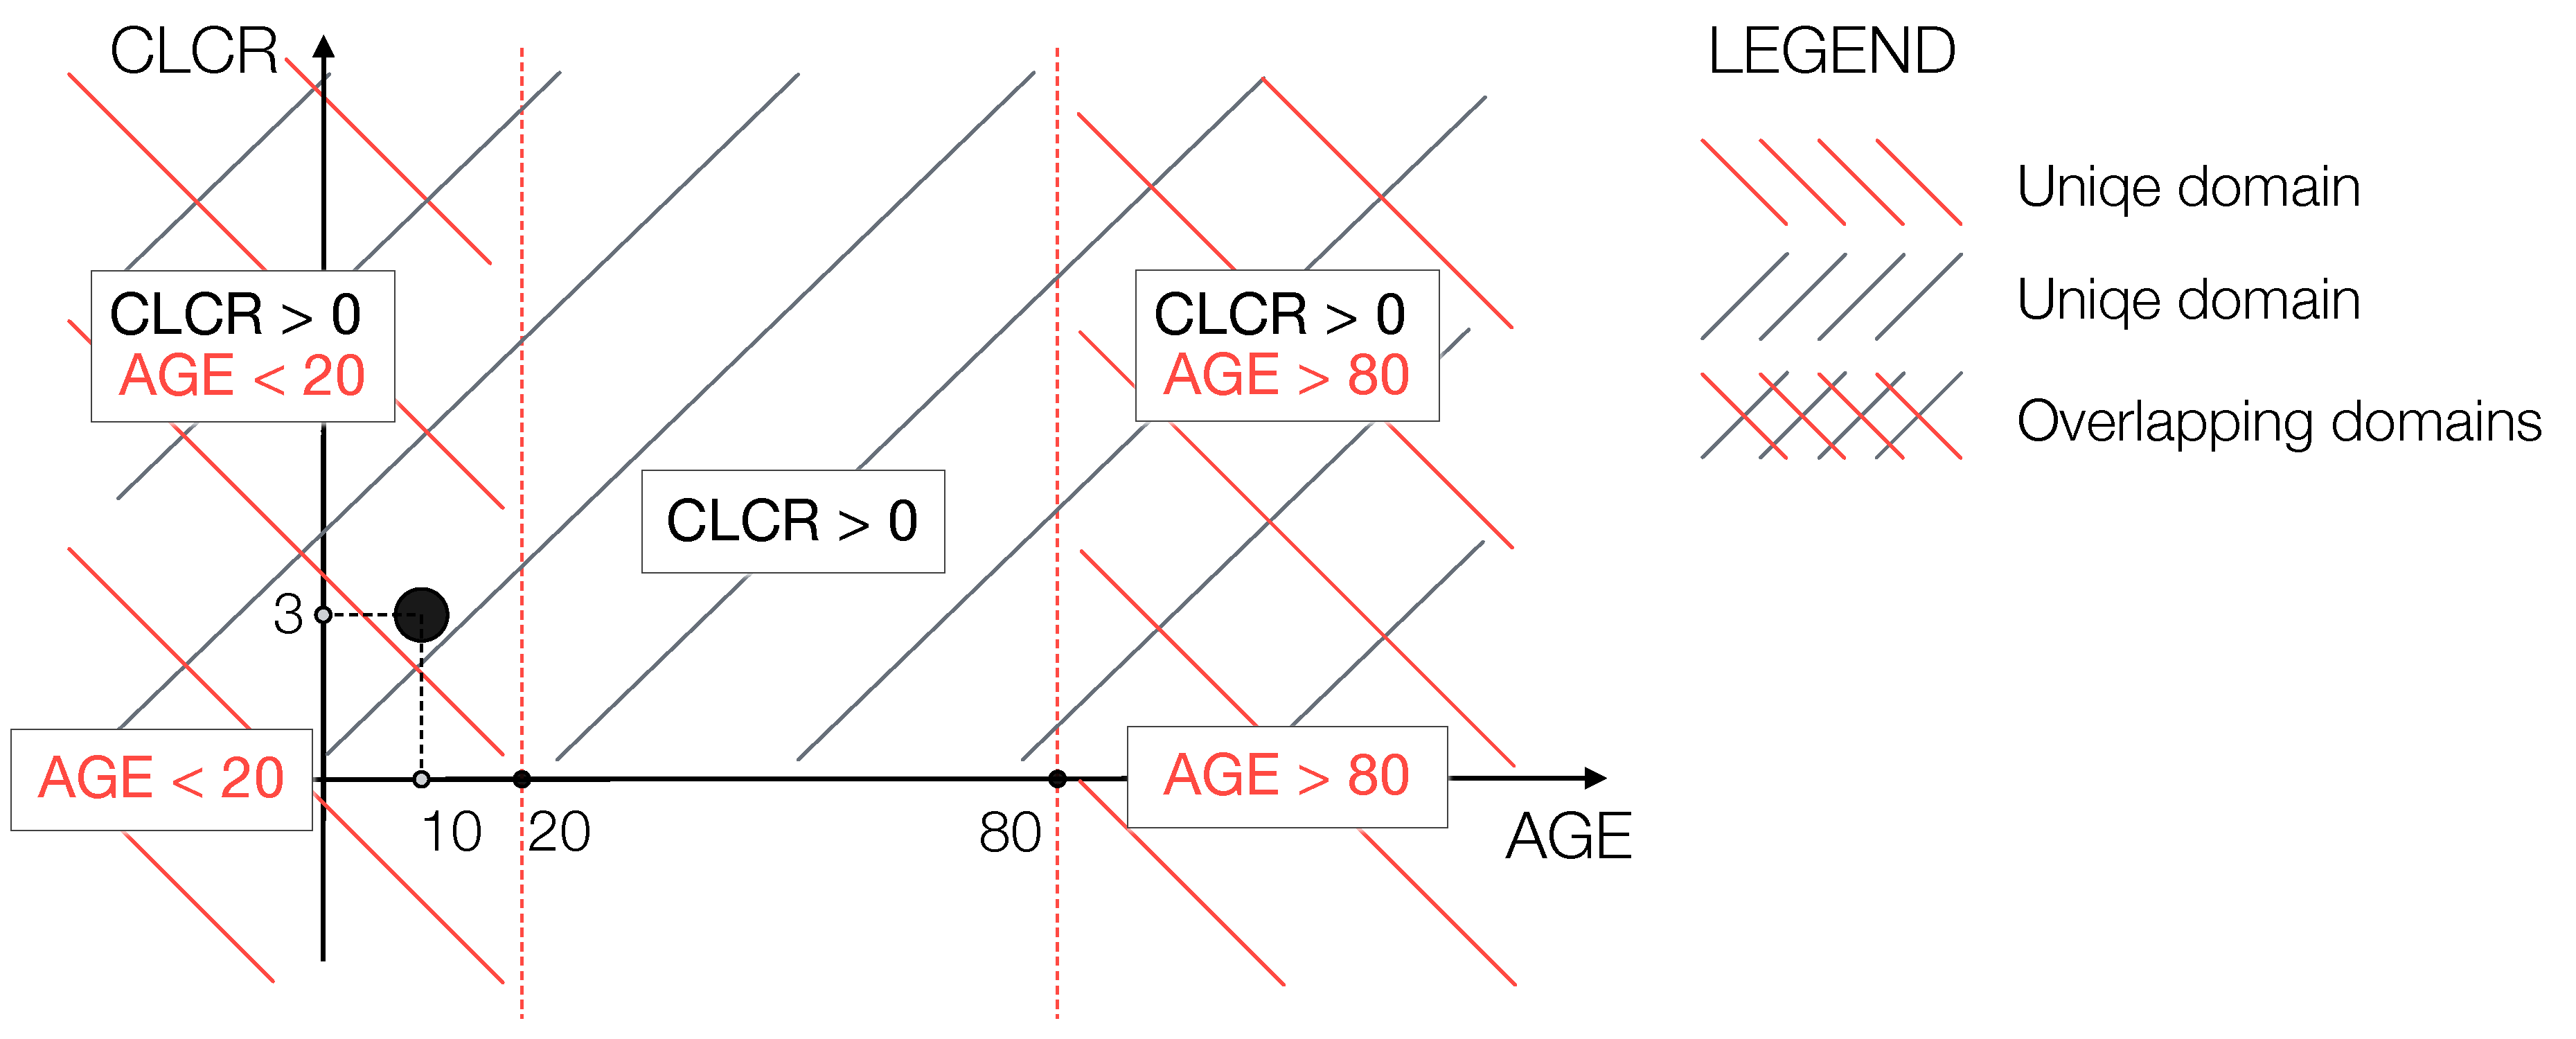
\includegraphics[width=140mm]{pics/CLCR_AGE.pdf}
 \caption{Domains for the conditions should be disjoint to avoid ambiguous
 assignments or the assignments have to be identical if domains overlap. 
 For example for CLCR=3 and AGE=10 the assignment of RF depends on the sequence 
 of the first two conditions.
 Because any domain declaration is allowed in PharmML, no automatic validity 
 check is performed,  the declarations are ultimately the responsibility of the modeller.}
 \label{fig:CLCR_AGE}
\end{figure}


\subsubsection*{Example 2}
The following conditional assignment 
%	{ ka = theta1 * exp(eta1)
%       ALAG1 = theta3} if Group == 1 
%     { ka = theta3 * exp(eta1)
%       ALAG1 = 0} if Group == 2
\begin{algorithmic}
	\If {$( Group = 1 )$}
	    \State $ka = \theta1 * \exp(\eta_1)$
	    \State $ALAG1 = \theta_3$
	\ElsIf {$( Group = 2 )$}
	    \State $ka = \theta_3 * \exp(\eta_1)$
	    \State $ALAG1 = 0$
	\EndIf
\end{algorithmic}
assumes that $ka$ and $ALAG1$ are declared first, i.e.
\lstset{language=XML}
\begin{lstlisting}
            <!-- declaration -->
            <IndividualParameter symbId="ka"/>
            <IndividualParameter symbId="ALAG1"/>
\end{lstlisting}
and then the conditional assignments can be specified
\lstset{language=XML}
\begin{lstlisting}
            <!-- conditional assignments -->
            <ConditionalStatement>
                <math:If>
                    <math:Condition>
                        <math:LogicBinop op="eq">
                            <ct:SymbRef symbIdRef="Group"/>
                            <ct:Int>1</ct:Int>
                        </math:LogicBinop>
                    </math:Condition>
                    <ct:AssignStatement op="eq">
                        <ct:SymbRef symbIdRef="ka"/>
                        <math:Binop op="times">
                            <ct:SymbRef symbIdRef="theta1"/>
                            <math:Uniop op="exp">
                                <ct:SymbRef symbIdRef="eta1"/>
                            </math:Uniop>
                        </math:Binop>
                    </ct:AssignStatement>
                    <ct:AssignStatement op="eq">
                        <ct:SymbRef symbIdRef="ALAG1"/>
                        <ct:SymbRef symbIdRef="theta3"/>
                    </ct:AssignStatement>
                </math:If>
                <math:ElseIf>
                    <math:Condition>
                        <math:LogicBinop op="eq">
                            <ct:SymbRef symbIdRef="Group"/>
                            <ct:Int>2</ct:Int>
                        </math:LogicBinop>
                    </math:Condition>
                    <ct:AssignStatement op="eq">
                    <!-- omitted assignments for ka and ALAG1 -->
                </math:ElseIf>
            </ConditionalStatement>
\end{lstlisting}


\subsubsection*{Example 3}
This example, from Fisher/Shafer NONMEM course, \cite{fisher2007shafer}, 
shows parameter assignment conditional on a categorical covariate.

\lstset{language=NM}
\begin{lstlisting}
	IF (SEX.EQ.0) THEN
		V= THETA(1) * EXP(ETA(1)) ; volume in men
	ELSE
		V= THETA(2) * EXP(ETA(1)) ; volume in women
	ENDIF
\end{lstlisting}
Declare first the covariate, Sex
\lstset{language=XML}
\begin{lstlisting}
        <CovariateModel blkId="cm1">
            <Covariate symbId="Sex">
                <Categorical>
                    <Category catId="1">
                        <ct:Name>Female</ct:Name>
                    </Category>
                    <Category catId="0"/>
                </Categorical>
            </Covariate>
\end{lstlisting}
and condition on it the assignment of the individual parameter, V. Note that 
parameter V needs to be declared first.
\lstset{language=XML}
\begin{lstlisting}
        <ParameterModel blkId="pm1">
            <IndividualParameter symbId="V"/>

            <PopulationParameter symbId="theta1"/>
            <PopulationParameter symbId="theta2"/>
\end{lstlisting}
followed by the conditional assignments 
\lstset{language=XML}
\begin{lstlisting}
            <RandomVariable symbId="eta1">
                <ct:VariabilityReference>
                    <ct:SymbRef symbIdRef="indiv"/>
                </ct:VariabilityReference>
                <!-- Distribution omitted -->
            </RandomVariable>
            <ConditionalStatement>
                <math:If>
                    <math:Condition>
                        <math:LogicBinop op="eq">
                            <ct:SymbRef symbIdRef="Sex"/>
                            <ct:CatRef catIdRef="0"/>
                        </math:LogicBinop>
                    </math:Condition>
                    <IndividualParameter symbIdRef="V">
                        <StructuredModel>
                            <PopulationValue>
                                <ct:Assign>
                                    <ct:SymbRef symbIdRef="theta1"/>
                                </ct:Assign>
                            </PopulationValue>
                            <RandomEffects>
                                <ct:SymbRef symbIdRef="eta1"/>
                            </RandomEffects>
                        </StructuredModel>
                    </IndividualParameter>
                </math:If>
                <math:Else>
                    <IndividualParameter symbIdRef="V">
                        <StructuredModel>
                            <PopulationValue>
                                <ct:Assign>
                                    <ct:SymbRef symbIdRef="theta2"/>
                                </ct:Assign>
                            </PopulationValue>
                            <RandomEffects>
                                <ct:SymbRef symbIdRef="eta1"/>
                            </RandomEffects>
                        </StructuredModel>
                    </IndividualParameter>
                </math:Else>
            </ConditionalStatement>
            ...
        </ParameterModel>
\end{lstlisting}
Note the attribute \xatt{symbIdRef}, used to reference the individual parameters
in each statement, which was not available for parameters or variables previously.

%\subsubsection*{Example 4}
%
%Source: Fisher/Shafer NONMEM course, \cite{fisher2007shafer}.
%
%\lstset{language=NM}
%\begin{lstlisting}
%	IF(CP.GE.PCP) THEN
%		SLOPE = (CP-PCP)/DT1
%		DELTA=DT1*SLOPE+(KE0*PCP-SLOPE)*(1-EXP(-KE0*DT1))/KE0
%	ELSE
%		SLOPE = (LOG(CP)-LOG(PCP))/DT1
%		DELTA=PCP*KE0/(KE0+SLOPE)*(EXP(DT1*SLOPE)-EXP(-KE0*DT1))
%	ENDIF
%\end{lstlisting}
%
%\lstset{language=XML}
%\begin{lstlisting}
%
%\end{lstlisting}
%
%\lstset{language=NM}
%\begin{lstlisting}
%IF (ROUTE.EQ.1) THEN ;extravascular parameters
%	FLGT = THETA(3) + ETA(2) ;only use additive error here to allow negative values
%	F1 = EXP(FLGT)/(1+EXP(FLGT)) ;logit transform to keep F between 0 and 1
%	KA = THETA(4)
%	ALAG1 = THETA(5)
%ELSE
%	F1 = 1
%	;others will be set to zero unless a value is specified here
%ENDIF
%\end{lstlisting}


\subsubsection*{Example 4 -- 'Three Compartment Infusion, Coefficient and Exponents'}

Source: Fisher/Shafer NONMEM course, \cite{fisher2007shafer}. The NMTRAN code for the 
structural and observation model reads
\lstset{language=NM}
\begin{lstlisting}
	; C1, C2, C3, L1, L2, L3, RATE, DUR defined elsewhere
	IF (TIME.LE.DUR) THEN
		TY1 = RATE*C1/L1*(1-EXP(-L1*TIME))
		TY2 = RATE*C2/L2*(1-EXP(-L2*TIME))
		TY3 = RATE*C3/L3*(1-EXP(-L3*TIME))
	ELSE
		TY1 = RATE*C1/L1*(1-EXP(-L1*DUR))*EXP(-L1*(TIME-DUR))
		TY2 = RATE*C2/L2*(1-EXP(-L2*DUR))*EXP(-L2*(TIME-DUR))
		TY3 = RATE*C3/L3*(1-EXP(-L3*DUR))*EXP(-L3*(TIME-DUR))
	ENDIF

	Y=(TY1+TY2+TY3)*(1+EPS(1)) ; Constant CV model
\end{lstlisting}
\bigskip
and in PharmML 
\lstset{language=XML}
\begin{lstlisting}
    <!-- STRUCTURAL MODEL -->
    <StructuralModel blkId="sm1">
        
        <ct:Variable symbolType="real" symbId="TY1"/>
        <ct:Variable symbolType="real" symbId="TY2"/>
        <ct:Variable symbolType="real" symbId="TY3"/>
        
        <ConditionalStatement>
            <math:If>
                <math:Condition>
                    <math:LogicBinop op="leq">
                        <ct:SymbRef symbIdRef="t"/>
                        <ct:SymbRef symbIdRef="DUR"/>
                    </math:LogicBinop>
                </math:Condition>
                <!-- TY1 = RATE*C1/L1*(1 - EXP(-L1*TIME)) -->
                <ct:AssignStatement op="eq">
                    <ct:SymbRef symbIdRef="TY1"/>
                    <!-- omitted RHS expression -->
                </ct:AssignStatement>
                <!-- TY2 = RATE*C2/L2*(1-EXP(-L2*TIME)) -->
                <ct:AssignStatement op="eq">
                    <ct:SymbRef symbIdRef="TY2"/>
                    <!-- omitted RHS expression -->
                </ct:AssignStatement>
                <ct:AssignStatement op="eq">
                    <ct:SymbRef symbIdRef="TY3"/>
                    <!-- omitted RHS expression -->
                </ct:AssignStatement>
            </math:If>
            <math:Else>
                <!-- TY1 = RATE*C1/L1*(1-EXP(-L1*DUR))*EXP(-L1*(TIME-DUR)) -->
                <ct:AssignStatement op="eq">
                    <ct:SymbRef symbIdRef="TY1"/>
                    <!-- omitted RHS expression -->
                </ct:AssignStatement>
                <!-- TY2 = RATE*C2/L2*(1-EXP(-L2*DUR))*EXP(-L2*(TIME-DUR)) -->
                <ct:AssignStatement op="eq">
                    <ct:SymbRef symbIdRef="TY2"/>
                    <!-- omitted RHS expression -->
                </ct:AssignStatement>
                <!-- TY3 = RATE*C3/L3*(1-EXP(-L3*DUR))*EXP(-L3*(TIME-DUR)) -->
                <ct:AssignStatement op="eq">
                    <ct:SymbRef symbIdRef="TY3"/>
                    <!-- omitted RHS expression -->
                </ct:AssignStatement>
                
            </math:Else>
        </ConditionalStatement>
\end{lstlisting}
\bigskip
The observation model is skipped here.


%\subsubsection*{Example 6 -- sleep model}
%
%\begin{itemize}
%\item
%Type of observed variable -- discrete / ordered categorical
%\item
%Category variable: $Y$
%\item
%Set of categories: $\{0,1,2,3,4,5\}$
%\item
%Probabilities
%\begin{align}
%& P(Y=1) = \exp(G1)/(1+\exp(G1)+\exp(G2)+\exp(G3)) \nonumber \\
%& P(Y=2) = \exp(G2)/(1+\exp(G1)+\exp(G2)+\exp(G3)) \nonumber \\
%& P(Y=3) = 0 \nonumber \\
%& P(Y=4) = 0 \nonumber \\
%& P(Y=5) = \exp(G3)/(1+\exp(G1)+\exp(G2)+\exp(G3)) \nonumber
%\end{align}
%\end{itemize}
%
%
%\lstset{language=NM}
%\begin{lstlisting}
%; Sleep model with multinomial logistic functions
%; Transitions from awake state
%; Categorical data model - 4 categories
%
%removed multiple assignments and definitions
%
%IF (STT.LE.BPsb.AND.SL.EQ.1) THEN
%    G1A=(TVG1A+ETA(1))*(BPsb-STT)/(BPsb-BPsa)+(TVG1A+ETA(1)+STE1b)*(STT-BPsa)/(BPsb-BPsa)
%	...
%    G1B=(TVG1B+ETA(1))*(BPsb-STT)/(BPsb-BPsa)+(TVG1B+ETA(1)+STE1b)*(STT-BPsa)/(BPsb-BPsa)
%	...
%    G1C=(TVG1C+ETA(1))*(BPsb-STT)/(BPsb-BPsa)+(TVG1C+ETA(1)+STE1b)*(STT-BPsa)/(BPsb-BPsa)
%	...
%ENDIF
%
%IF (STT.GT.BPsb.AND.SL.EQ.1) THEN
%    G1A=(TVG1A+ETA(1)+STE1b)*(BPsc-STT)/(BPsc-BPsb)+(TVG1A+ETA(1)+STE1c)*(STT-BPsb)/(BPsc-BPsb)
%    ...
%
%    G1B=(TVG1B+ETA(1)+STE1b)*(BPsc-STT)/(BPsc-BPsb)+(TVG1B+ETA(1)+STE1c)*(STT-BPsb)/(BPsc-BPsb)
%    ...
%
%    G1C=(TVG1C+ETA(1)+STE1b)*(BPsc-STT)/(BPsc-BPsb)+(TVG1C+ETA(1)+STE1c)*(STT-BPsb)/(BPsc-BPsb)
%    ...
%ENDIF
%
%
%IF (TIME.GE.BPA.AND.TIME.LE.BPB.AND.SL.EQ.1) THEN
%    G1=G1A*(BPB-TIME)/(BPB-BPA)+G1B*(TIME-BPA)/(BPB-BPA)
%    ...
%ENDIF
%
%IF (TIME.GT.BPB.AND.TIME.LE.BPC.AND.SL.EQ.1) THEN
%    G1=G1B*(BPC-TIME)/(BPC-BPB)+G1C*(TIME-BPB)/(BPC-BPB)
%    ...
%ENDIF
%
%
%  IF (TIME.GE.BP1.AND.TIME.LE.BP2.AND.SL.EQ.0) THEN - sleep part of the night; from 1 < x < 2
%    G1=(TVG11+ETA(4))*(BP2-TIME)/(BP2-BP1)+(TVG12+ETA(4))*(TIME-BP1)/(BP2-BP1)
%    ...
%  ENDIF
%
%  IF (TIME.GT.BP2.AND.TIME.LE.BP3.AND.SL.EQ.0) THEN - sleep part of the night; from 2 < x < 3
%    G1=(TVG12+ETA(4))*(BP3-TIME)/(BP3-BP2)+(TVG13+ETA(4))*(TIME-BP2)/(BP3-BP2)
%    ...
%  ENDIF
%\end{lstlisting}
%
%
%%%%%%%%%%%%%%%%%%%%%%%%%%%%%%%%%%%%%%%%%%%%%%%%%%%%%%%
\section{Nested piecewise}
\label{sec:nestedPiecewise}
Nesting of piecewise statements was not supported so far, here a typical one

\bigskip
$f(x) = \left\{ 
\begin{array}{ccl}
\left\{ 
\begin{array}{rcl}
1 & \mbox{for} & x<1 \\ 
2 & \mbox{else} 
\end{array}\right. & \mbox{for} & x>0 \\ 
3 & \mbox{else} 
\end{array}\right.$
\bigskip \\
implemented in PharmML as the following snippet shows
\lstset{language=XML}
\begin{lstlisting}
        <ct:Variable symbolType="real" symbId="f">
            <ct:Assign>
                <ct:Piecewise>
                    <math:Piece>
                        <!-- nested piecewise -->
                        <math:Piecewise>
                            <math:Piece>
                                <ct:Real>1</ct:Real>
                                <math:Condition>
                                    <math:LogicBinop op="lt">
                                        <ct:SymbRef symbIdRef="x"/>
                                        <ct:Real>1</ct:Real>
                                    </math:LogicBinop>
                                </math:Condition>
                            </math:Piece>
                            <math:Piece>
                                <ct:Real>2</ct:Real>
                                <math:Condition>
                                    <math:Otherwise/>
                                </math:Condition>
                            </math:Piece>
                        </math:Piecewise>
                        <math:Condition>
                            <math:LogicBinop op="gt">
                                <ct:SymbRef symbIdRef="x"/>
                                <ct:Real>0</ct:Real>
                            </math:LogicBinop>
                        </math:Condition>
                    </math:Piece>
                    <math:Piece>
                        <ct:Real>3</ct:Real>
                        <math:Condition>
                            <math:Otherwise/>
                        </math:Condition>
                    </math:Piece>
                </ct:Piecewise>
            </ct:Assign>
        </ct:Variable>
\end{lstlisting}


%%%%%%%%%%%%%%%%%%%%%%%%%%%%%%%%%%%%%%%%%%%%%%%%%%%%%%%
\section{Probability functions support}
\label{sec:probabFunctions}
Following probability functions are available 
\begin{itemize}
\item 
CDF(x) -- cumulative distribution function, \xelem{CDF}
\item 
PDF(x) -- probability density function, \xelem{PDF}
\item 
HF(x) -- hazard function, \xelem{HF}
\item 
SF(x) -- survival function, \xelem{SF}
\end{itemize}
\bigskip
The implementation of these probability functions is straightforward, despite
their often very complex expressions which are only referred to, and 
requires the use of the 
\begin{enumerate}
\item 
according XML element, e.g. \xelem{CDF}
\item 
specification of the distribution of interest and
\item 
(optional) function argument, x, which can be any expression.
\end{enumerate}
The introduction of these generic elements allows to use any of the 
ProbOnto univariate continuos distributions, \cite{ProbOnto:2015a}.
Consider for example the cumulative distribution
function, \emph{PHI}, of the standard normal distribution with mean 0
and standard deviation 1 which the two basic function read
\begin{align*}
\mbox{PDF}:  \quad f(x) &= \frac{e^{-\frac{1}{2} x^2}}{\sqrt{2\pi}} \nonumber \\
\mbox{CDF}:  \quad F(x) &= \frac12\left[1 + \text{erf}\left( \frac{x}{\sqrt{2}}\right)\right]  \quad \mbox{with} \quad \text{erf}(z) = \frac{2}{\pi}\int_0^z e^{-t^2} dt\nonumber
\end{align*}
where \emph{erf} is the error function\footnote{\url{mathworld.wolfram.com/Erf.html}}.

\bigskip
The abbreviated XML code explains its encoding reduced to the 
specification of the distribution function, the code name, \emph{StandardNormal1}, 
and the optional argument
\lstset{language=XML}
\begin{lstlisting}
    <ct:Variable symbolType="real" symbId="PHI">
        <ct:Assign>
            <math:CDF>
                <math:Distribution>
                    <po:ProbOnto name="StandardNormal1"/>
                </math:Distribution>
                <ct:Assign>
                <!-- x, argument -->
                </ct:Assign>
            </math:CDF>
        </ct:Assign>
    </ct:Variable>
\end{lstlisting}
Note, that CDF of the standard normal is straightforward as it doesn't
requiere specification of parameters, which are by default 
$mean\!=\!0$ and $stdev\!=\!1$. 
The use of probability functions is explained in the following examples. 
%in the context of a model proposed for handling data below the level 
%of quantification, BLQ, \cite{Beal:2001}.


\subsection{Example 1 -- basic example}
Source: Part VII, Help Guide of the \cite{NONMEM:2009}.
The cumulative distribution function, \emph{PHI}, of the standard normal 
distribution with mean 0 and standard deviation 1, may be used as in 
this is basic example
\lstset{language=NM}
\begin{lstlisting}
	A=THETA(1)*EXP(ETA(1))
	B=PHI(A)
\end{lstlisting}

\begin{longtable}{cc}
\hline
$A = \theta_1 \exp(\eta_1)$
&
\lstset{language=XML}
\begin{lstlisting}
<IndividualParameter symbId="A">
    <ct:Assign>
        <math:Binop op="times">
            <ct:SymbRef symbIdRef="THETA1"/>
            <math:Uniop op="exp">
                <ct:SymbRef symbIdRef="ETA1"/>
            </math:Uniop>
        </math:Binop>
    </ct:Assign>
</IndividualParameter>
\end{lstlisting}
\\
 \hline
$B = \mbox{CDF}(A)$
 &
 \lstset{language=XML}
\begin{lstlisting}
        <IndividualParameter symbId="B">
            <ct:Assign>
                <math:CDF>
                    <math:Distribution>
                        <po:ProbOnto name="StandardNormal1"/>
                    </math:Distribution>
                    <ct:Assign>
                        <ct:SymbRef symbIdRef="A"/>
                    </ct:Assign>
                </math:CDF>
            </ct:Assign>
        </IndividualParameter>
\end{lstlisting}
\\
\hline
\caption{Encoding of the basic example using cumulative distribution function, CDF.}
\end{longtable}%


\subsection{Example 2 -- M3-method for handling of BLQ data}
According to \cite{Beal:2001}, the likelihood for a censored observation 
at time t, is given by 
\begin{align*}
l(t) = \Phi((QL - f(t))/\sqrt{g(t)}), \quad \mbox{with } \Phi \mbox{ the CDF of the } \mathcal{N}(0,1)
\end{align*}
which is the probability that the observation is BQL, (i.e., is between 
$-\infty$ and quantification limit, QL.\\
An example how to implement the so-called M3-method for handling 
of such data
provides the tutorial by \cite{Mould_partII:2013} with the following 
NMTRAN from the supplementary material of the paper.
\lstset{language=NM}
\begin{lstlisting}
	$ERROR ; Beal Method 3
	;residual error is coded here using THETA's rather than EPS's
	ADD = THETA(6)
	PROP = F*THETA(7)
	SD = SQRT(ADD*ADD+PROP*PROP) ; combined error model
	LLOQ=0.05 ; lower limit of quantification
	IF (BLQ.EQ.0) THEN
		F_FLAG=0 ;regular likelihood for measured concentrations
		Y = F + SD*EPS(1)
	ENDIF
	IF (BLQ.EQ.1) THEN
		F_FLAG=1 ;probability that F is less than LLOQ for missing concentrations
		Y=PHI((LLOQ-F)/SD)
	ENDIF
\end{lstlisting}
While the first couple of lines are standard and will be omitted
here, the encoding of the essential line with PHI function, 
Y=PHI((LLOQ-F)/SD), is shown in the following snippet
\lstset{language=XML}
\begin{lstlisting}
        <ObservationModel blkId="om4">
            <ContinuousData>
	        <!-- Y=PHI((LLOQ-F)/SD) -->
                <General symbId="Y">
                    <ct:Assign>
                        <math:CDF>
                            <math:Distribution>
                                <po:ProbOnto name="StandardNormal1"/>
                            </math:Distribution>
                            <ct:Assign>
                                <math:Binop op="divide">
                                    <math:Binop op="minus">
                                        <ct:SymbRef symbIdRef="LLOQ"/>
                                        <ct:SymbRef blkIdRef="sm1" symbIdRef="F"/>
                                    </math:Binop>
                                    <ct:SymbRef symbIdRef="SD"/>
                                </math:Binop>
                            </ct:Assign>
                        </math:CDF>
                    </ct:Assign>
                </General>
            </ContinuousData>
        </ObservationModel>
\end{lstlisting}
As noted before, the encoding of the CDF of the standard normal doesn't
require the specification of default, $mean\!=\!0$ and $stdev\!=\!1$, parameters. 

\subsection{Example 3 -- TTE model}
\label{subsec:TTEmodel}
The probability functions turn out to be very useful also in encoding 
of time-to-event data. While so far encoding of hazard or survival functions
formulas was the only option to defined such models, they offer a quick 
and safe way to encode often complex function of interest as the following 
example demonstrates for a Weibull model 
\lstset{language=XML}
\begin{lstlisting}
            <HazardFunction symbId="h2">
                <ct:Assign>
                    <math:HF>
                        <math:Distribution>
                            <ProbOnto xmlns="http://www.pharmml.org/probonto/ProbOnto" name="Weibull1">
                                <Parameter name="scale">
                                    <ct:Assign>
                                        <ct:SymbRef blkIdRef="pm1" symbIdRef="beta"/>
                                    </ct:Assign>
                                </Parameter>
                                <Parameter name="shape">
                                    <ct:Assign>
                                        <ct:SymbRef blkIdRef="pm1" symbIdRef="lambda"/>
                                    </ct:Assign>
                                </Parameter>
                            </ProbOnto>
                        </math:Distribution>
                        <!-- function argument is optional -->
                        <ct:Assign>
                            <ct:SymbRef symbIdRef="t"/>
                        </ct:Assign>
                    </math:HF>
                </ct:Assign>   
            </HazardFunction>
\end{lstlisting}

%
%\newpage
%
%\begin{figure}[ht!]
%\centering
%  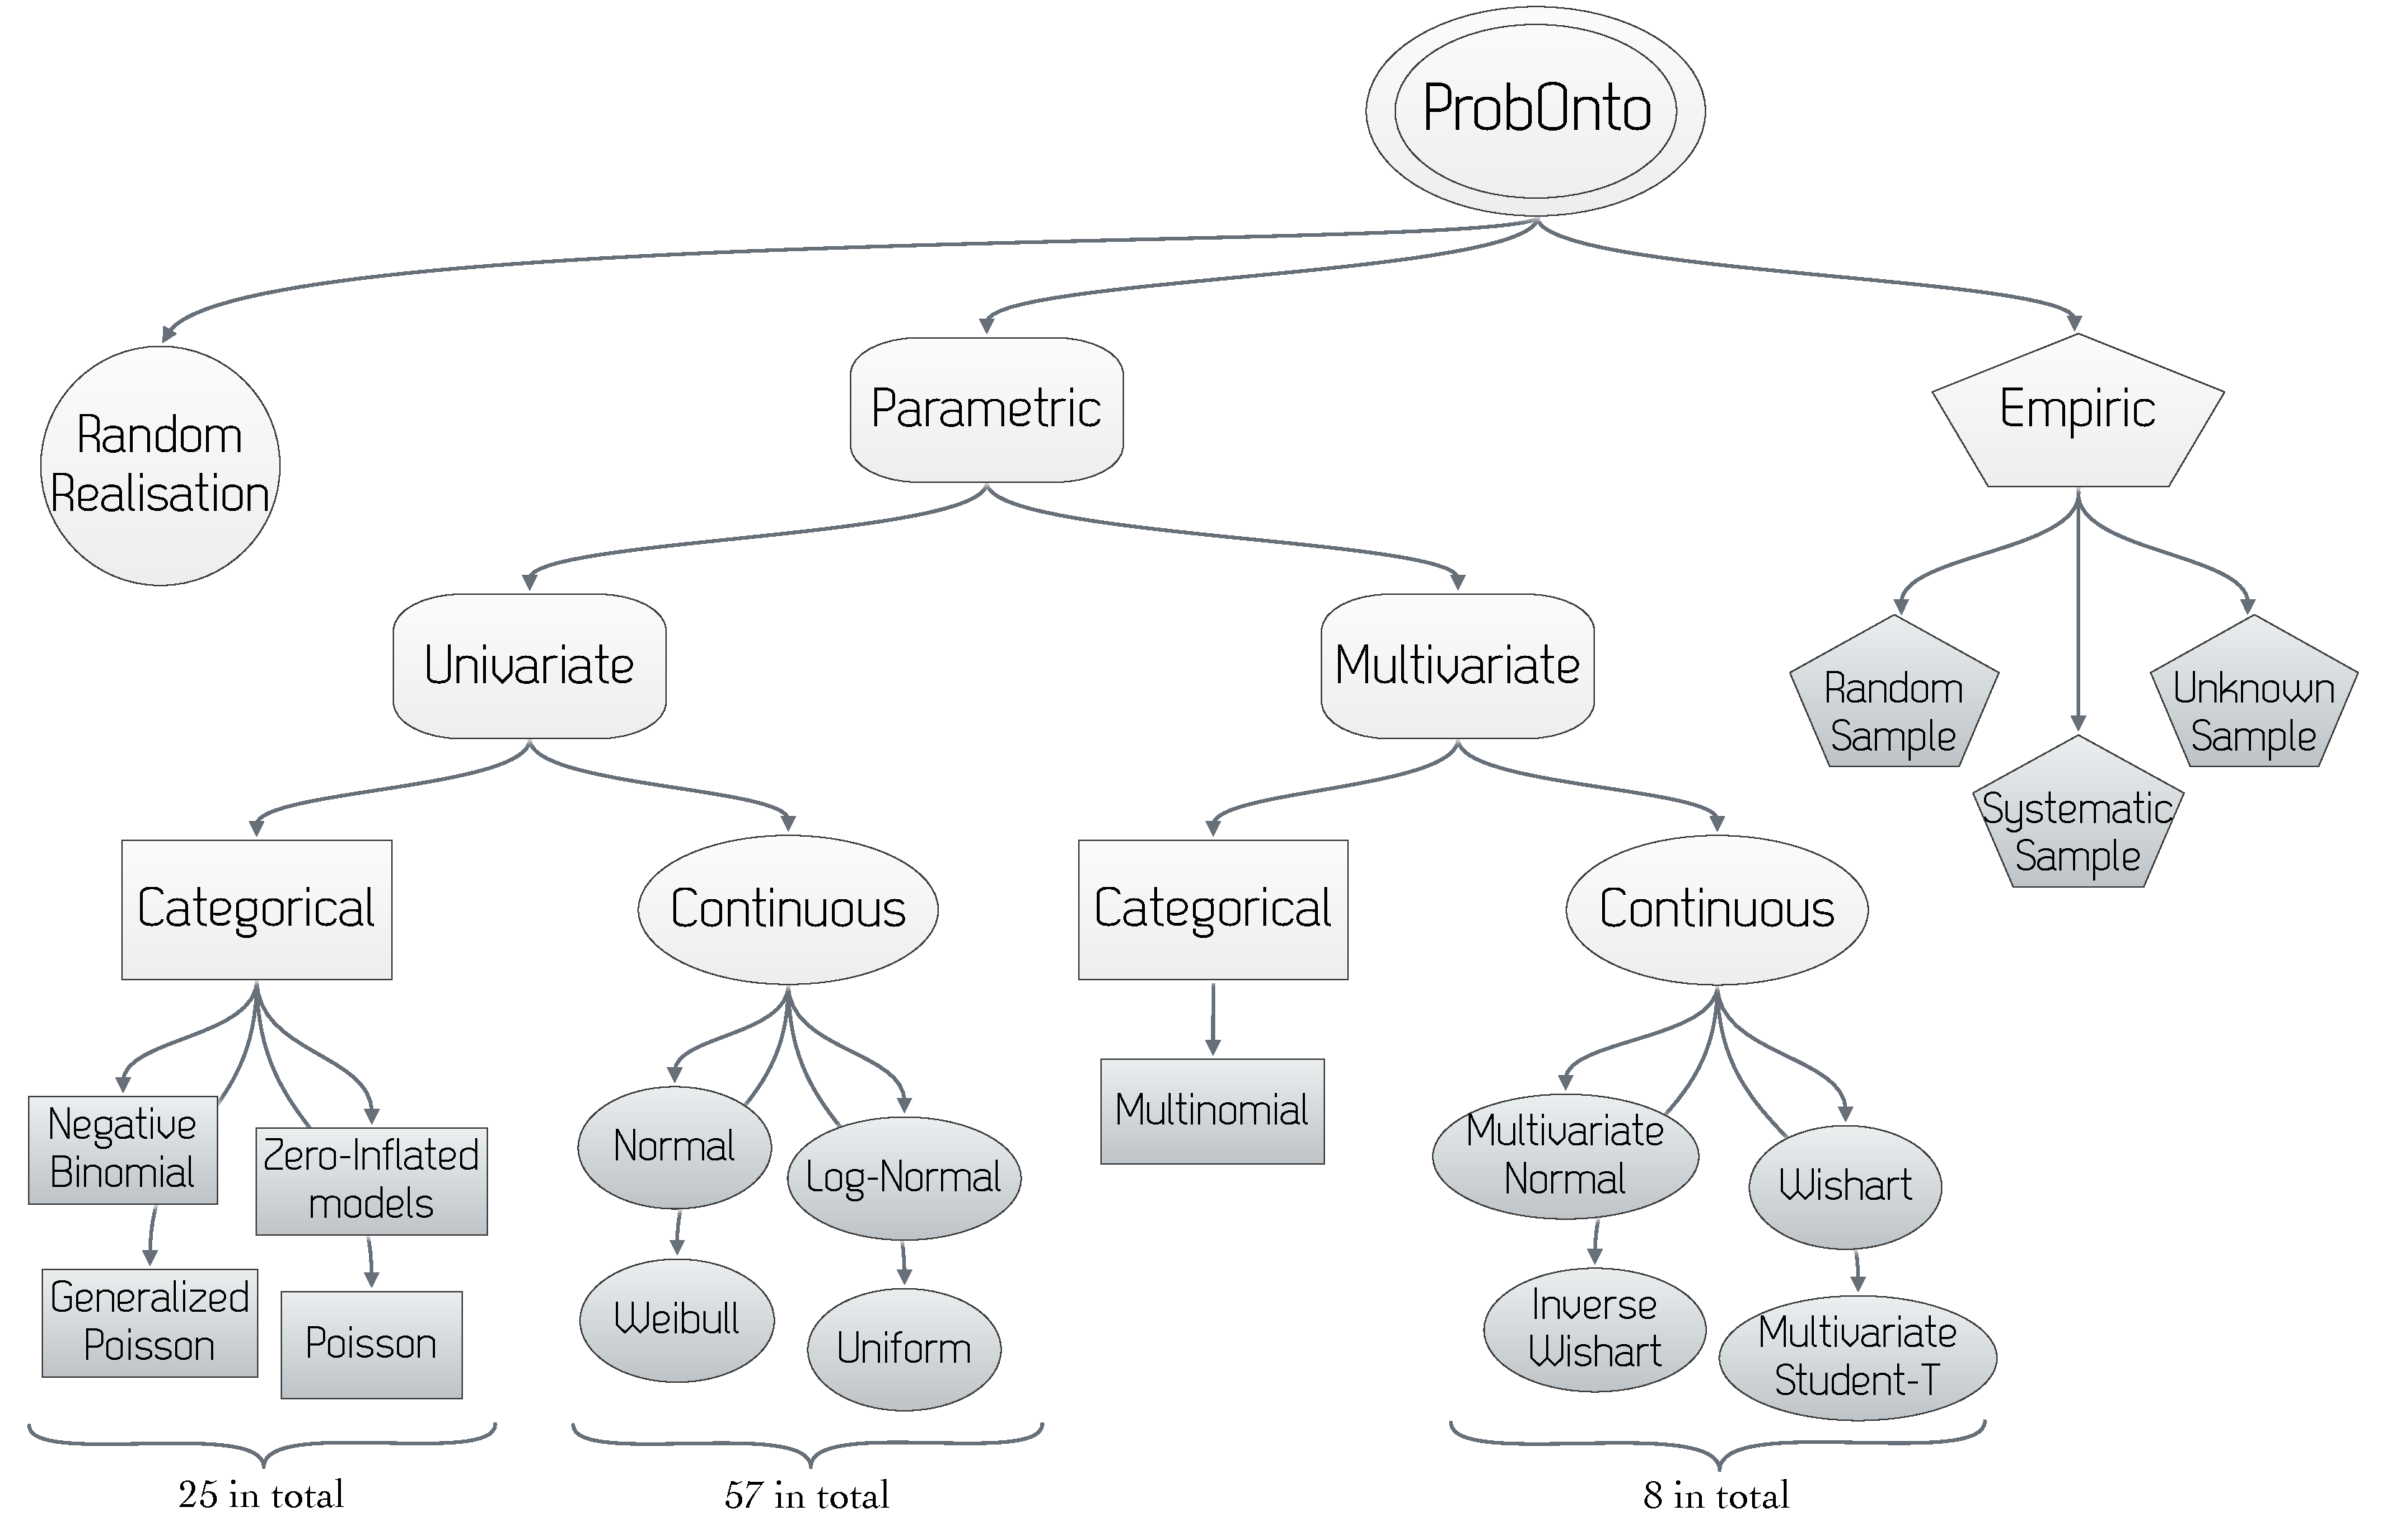
\includegraphics[width=140mm]{pics/ProbOnto_tree}
% \caption{Mapping of BLQ data and observation models.}
% \label{fig:BLQmapping}
%\end{figure}

\begin{figure}[ht!]
\centering
  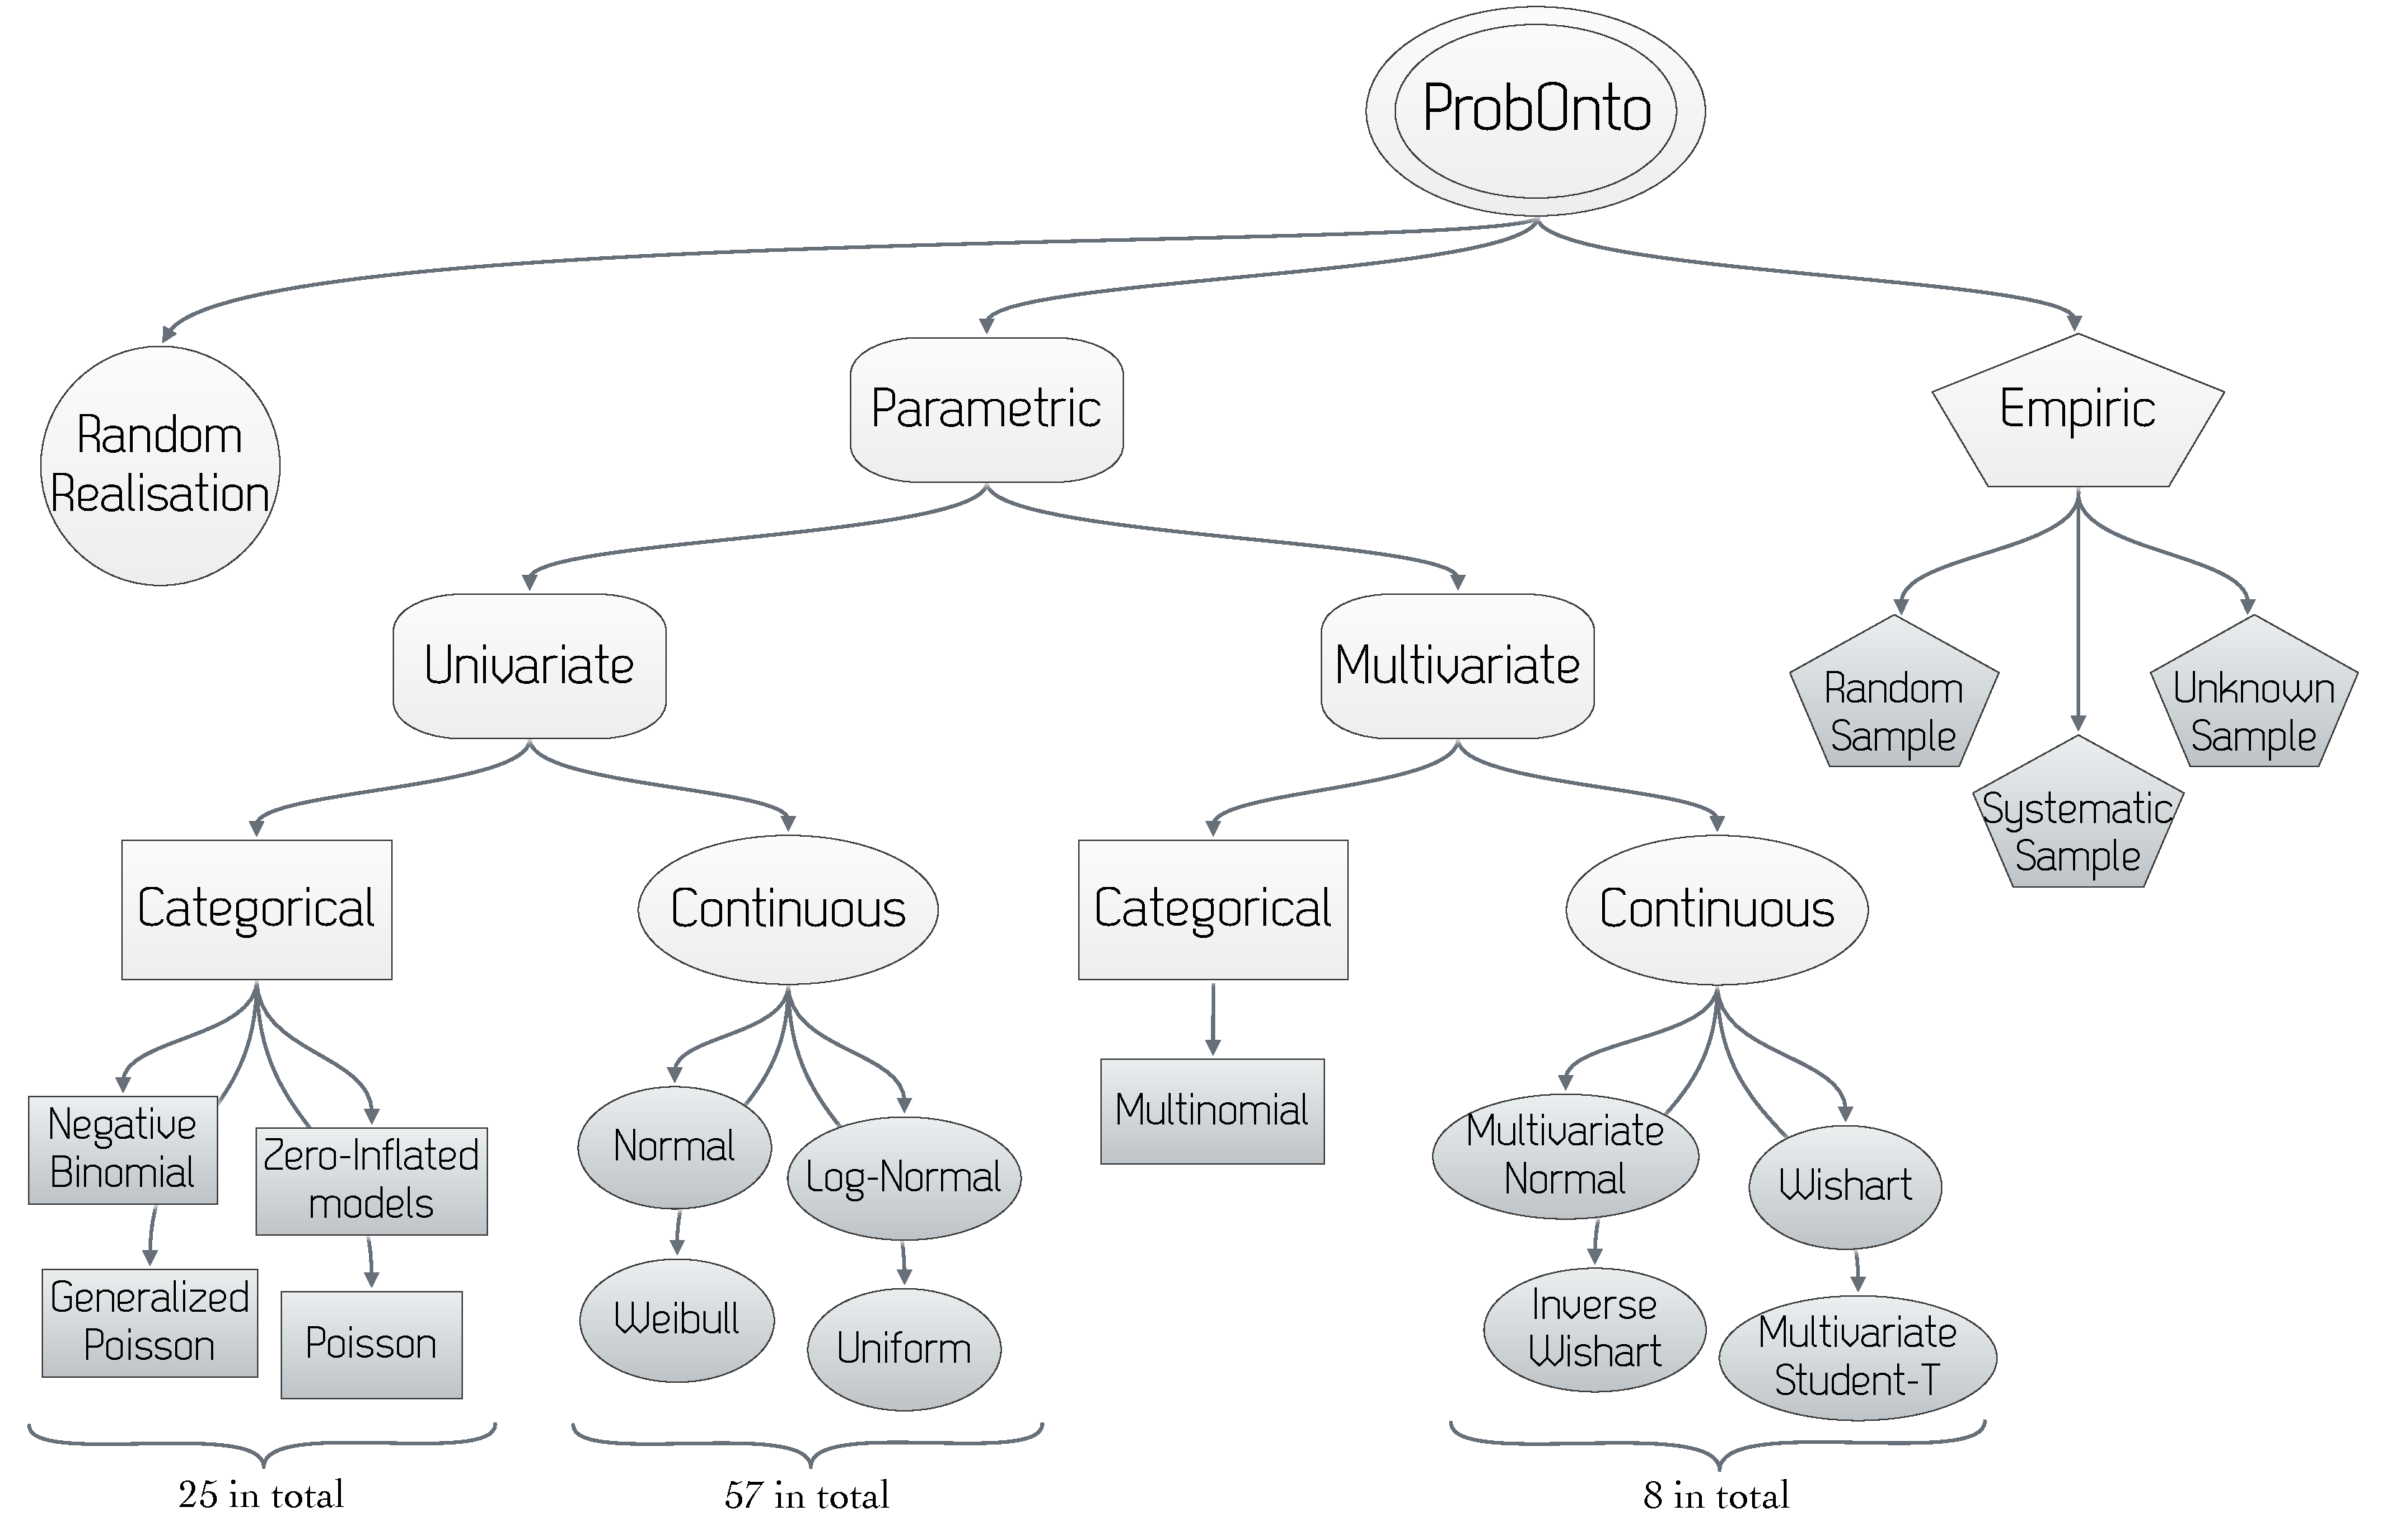
\includegraphics[width=140mm]{pics/ProbOnto_tree}
 \caption{ProbOnto tree -- showing the current structure. For brevity only few 
 distributions per category are listed.}
 \label{fig:ProbOnto_tree}
\end{figure}


%%%%%%%%%%%%%%%%%%%%%%%%%%%%%%%%%%%%%%%%%%%%%%%%%%%%%%%
\section{Samples -- empirical distributions support}
\label{sec:nonParamDistribs}

%ADD FIGURE \\
%ADD FIGURE \\
%ADD FIGURE \\
%ADD FIGURE \\
%and explanation about sample encoding, place where its encoded and its mapping

When formulating models it is often not possible to specify a probability 
distribution using a parametric one because its defining
function is not known. Instead, a set of values can be considered 
as constituting a distribution model. According extensions were required
in ProbOnto and PharmML.

\emph{Samples} are sets of realisations obtained from a known or unknown 
distribution. Following UncertML \cite{uncertml3:2014} we distinguish between 
\begin{itemize}
\item 
Random sample, \xelem{RandomSample}
\item 
Systematic sample, \xelem{SystematicSample}
\item 
Unknown sample, \xelem{UnknownSample}
\end{itemize}
The only (optional) parameter is 
\begin{itemize}
\item 
\xatt{weight} -- to encode weighting given to each realisation.
\end{itemize}
The main type which should be used for our purposes is the first one defined as
\begin{description}
\item[Random Sample] -- a set of independent realisations, $x_i$, drawn from 
a probability distribution $p(x)$ (or alternatively a population where every 
member has an equal chance of being drawn, but is randomly selected). 
The sample will typically be obtained using some form of simulation algorithm 
for distributions using a random number generator. 
\end{description}
See also ProbOnto specification for more details, \cite{ProbOnto:2015a}.

%%%%%%%%%%%%%%%%%%%%%%%%%%%%%%%%%%%%%%%%%%%%%%%%%%%%%%%
\subsection{Two modes of operation}
There are two ways samples can be encoded in PharmML, Table \ref{tab:twoOptionsForSamples}:
\begin{itemize}
\item 
Option 1: Data stored together with the corresponding parameter
\item 
Option 2: Data stored in \xelem{TrialDesign}
\end{itemize}
Both encoding result in exact the same model. In both cases the mapping 
between data columns and parameters is essential to assure complete model 
definition (if only one column is given, mapping is optional, see Table \ref{tab:twoOptionsForSamples}
alternative \textbf{Option 1} version). 
\newpage
\begin{longtable}{c}
\hline
\hline
\textbf{Option 1}: Data stored together with parameter \\
\hline
\lstset{language=XML}
\begin{lstlisting}
    <ParameterModel blkId="PM1">
        <PopulationParameter symbId="POP_K">
            <Distribution>
                <po:ProbOnto name="RandomSample">
                    <po:ColumnMapping>
                        <ds:ColumnRef columnIdRef="POP_K_sample"/>
                        <ct:SymbRef symbIdRef="POP_K"/>
                    </po:ColumnMapping>
                    <ds:DataSet>
                        <ds:Definition>
                            <ds:Column columnId="POP_K_sample" valueType="real" columnNum="1"/>
                        </ds:Definition>
                        <ds:Table>
                            <ds:Row><ct:Real>0.10</ct:Real></ds:Row>
                            <!-- other values omitted -->
                        </ds:Table>
                    </ds:DataSet>
                </po:ProbOnto>
            </Distribution>
        </PopulationParameter>

        <!-- ALTERNATIVE - short version -->
        <PopulationParameter symbId="POP_K">
            <Distribution>
                <po:ProbOnto name="RandomSample">
                    <ds:DataSet>
                        <ds:Table>
                            <ds:Row><ct:Real>0.10</ct:Real></ds:Row>
                            <!-- other values omitted -->
                        </ds:Table>
                    </ds:DataSet>
                </po:ProbOnto>
            </Distribution>
        </PopulationParameter>
    </ParameterModel>
\end{lstlisting}
\\
\hline
\textbf{Option 2}: Data stored in \xelem{TrialDesign} 
\\
\hline
\lstset{language=XML}
\begin{lstlisting}
<!-- PART 1 -->
<ParameterModel blkId="PM2">
    <PopulationParameter symbId="POP_K">
        <Distribution>
            <po:ProbOnto name="RandomSample"/>                    
        </Distribution>
    </PopulationParameter>            
</ParameterModel>

<!-- PART 2 -->
<TrialDesign xmlns="http://www.pharmml.org/pharmml/0.7/TrialDesign">    
    <ExternalDataSet oid="RdataSet">
        <ColumnMapping>
            <ds:ColumnRef columnIdRef="POP_K_sample"/>
            <ct:SymbRef blkIdRef="PM2" symbIdRef="POP_K"/>
        </ColumnMapping>
        <ds:DataSet>
            <ds:Definition>
                <ds:Column columnId="POP_K_sample" valueType="real" columnNum="1"/>
            </ds:Definition>
            <ds:Table>
                <ds:Row><ct:Real>0.10</ct:Real></ds:Row>
                <!-- other values omitted -->
            </ds:Table>
        </ds:DataSet>
    </ExternalDataSet>
</TrialDesign>
\end{lstlisting}
\\
\hline
\caption{Two way to encode samples. 
\textbf{Option 1}: data stored together with parameter declaration in \xelem{ModelDefinition}.
Two version are shown: (top) with full data/model mapping and dataset column 
declaration, (bottom) short form when only one dataset is required - mapping and 
column declaration are redundant. \textbf{Option 2}: data stored in the \xelem{TrialDesign} --
mapping is mandatory even for single column.}
\label{tab:twoOptionsForSamples}
\end{longtable}%

%\begin{longtable}{cc}
%\hline
%\hline
%  \multicolumn{2}{c}{Option 2: Data stored in \xelem{TrialDesign}} 
%\\
%\hline
%\lstset{language=XML}
%\begin{lstlisting}
%<!-- PART 1 -->
%<ParameterModel blkId="PM2">
%    <PopulationParameter symbId="POP_K">
%        <Distribution>
%            <po:ProbOnto name="RandomSample"/>                    
%        </Distribution>
%    </PopulationParameter>            
%</ParameterModel>
%
%<!-- PART 2 -->
%<TrialDesign xmlns="http://www.pharmml.org/pharmml/0.7/TrialDesign">    
%    <ExternalDataSet oid="RdataSet">
%        <ColumnMapping>
%            <ds:ColumnRef columnIdRef="POP_K_sample"/>
%            <ct:SymbRef blkIdRef="PM2" symbIdRef="POP_K"/>
%        </ColumnMapping>
%        <ds:DataSet>
%            <ds:Definition>
%                <ds:Column columnId="POP_K_sample" valueType="real" columnNum="1"/>
%            </ds:Definition>
%            <ds:Table>
%                <ds:Row><ct:Real>0.10</ct:Real></ds:Row>
%                <ds:Row><ct:Real>0.23</ct:Real></ds:Row>
%                <ds:Row><ct:Real>0.3</ct:Real></ds:Row>
%            </ds:Table>
%        </ds:DataSet>
%    </ExternalDataSet>
%</TrialDesign>
%\end{lstlisting}
%\\
%\hline
%\caption{Option 2: data stored in the \xelem{TrialDesign}.}
%\label{tab:twoOptionsForSamples}
%\end{longtable}%


%%%%%%%%%%%%%%%%%%%%%%%%%%%%%%%%%%%%%%%%%%%%%%%%%%%%%%%
\subsection{Mapping without \xatt{weight} parameter}

%%%%%%%%%%%%%%%%%%%%%%%%%%%%%%%%%%%%%%%%%%%%%%%%%%%%%%%
\subsubsection*{Option 1}
\label{subsec:exp2}
(See the use case \emph{bayesianHierarchical/example3423.xml} using this option.)\\

Sometimes the \xatt{weight} parameter is not defined and the assumption 
is that all values are equally probable with $p=1/n$ where
$n$ equal the row numbers, see Table \ref{tab:randomSample_withoutWeight}.

\begin{longtable}{c}
\hline
\hline
POP\_V \\
\hline
5.050013 \\
5.064166 \\
5.078318 \\ 
... \\
\hline
\caption{Test data set represented using equiprobable samples. Because no \xatt{weight} parameter
is defined, the assumption is that all values are equally probable with $p=1/n$ where
$n$ is equal the row numbers.}
\label{tab:randomSample_withoutWeight}
\end{longtable}%

\lstset{language=XML}
\begin{lstlisting}
    <PopulationParameter symbId="POP_K">
        <Distribution>
            <po:ProbOnto name="RandomSample">
                <ds:DataSet>
                    <ds:Table>
                        <ds:Row><ct:Real>0.10</ct:Real></ds:Row>
                        <ds:Row><ct:Real>0.23</ct:Real></ds:Row>
                        <ds:Row><ct:Real>0.3</ct:Real></ds:Row>
                    </ds:Table>
                    <!-- <ds:ExternalFile oid="sxtData">
                        <ds:path>POP_K_sample.csv</ds:path>
                    </ds:ExternalFile>-->
                </ds:DataSet>
            </po:ProbOnto>
        </Distribution>
    </PopulationParameter>
\end{lstlisting}
Here the short version was used which is applicable when only one data 
column in required. Providing mapping and column definition is in such
cases redundant, unless the data is stored in \xelem{TrialDesign}, see below.

\subsubsection*{Option 2}
\label{subsec:exp1}
%Sometimes the \xatt{weight} parameter is not defined and the assumption 
%is that all values are equally probable with $p=1/n$ where
%$n$ equal the row numbers, see Table \ref{tab:randomSampleExternalwithoutWeight}
%and Figure \ref{fig:Mapping_singleParam_noWeights}.
Figure \ref{fig:Mapping_singleParam_noWeights} shows how to store and
map dataset  with samples declared in \xelem{TrialDesign} to a parameter 
defined in \xelem{ParameterModel}, here $POP\_V$. In this case column mapping and 
column declaration are required.


\begin{figure}[ht!]
\centering
  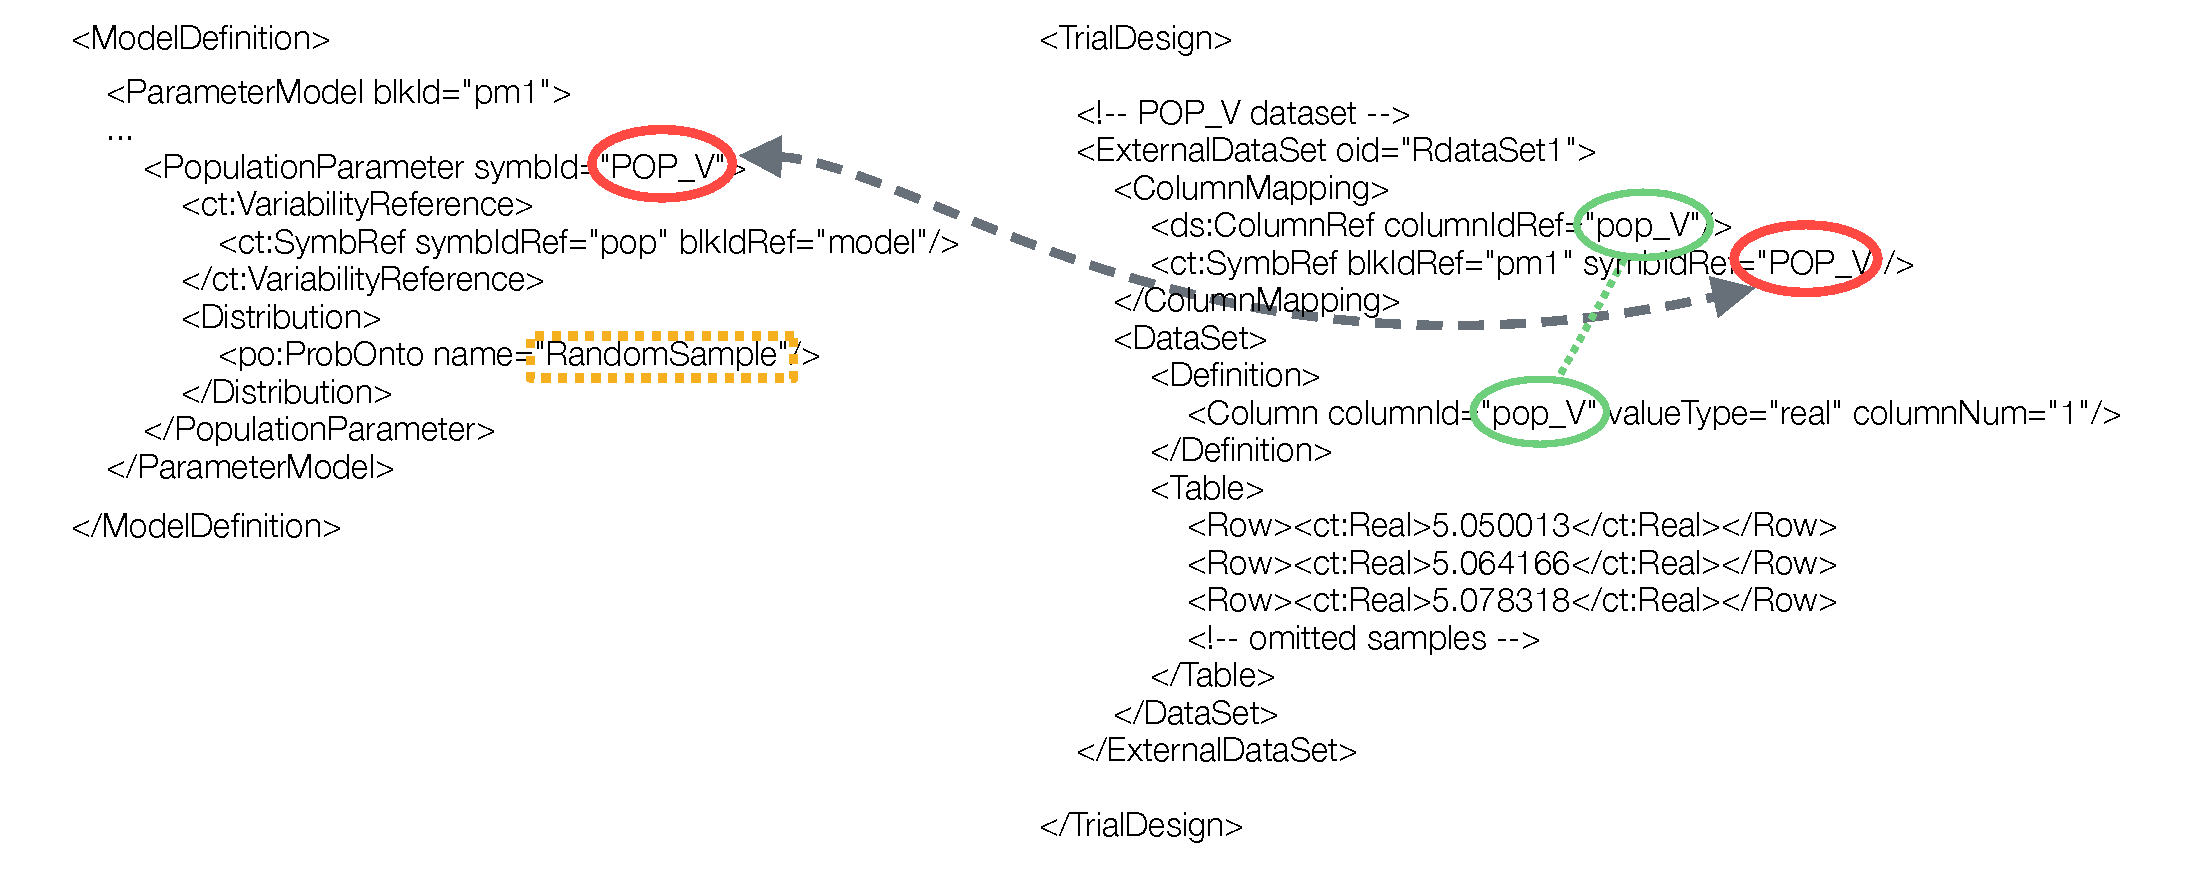
\includegraphics[width=160mm]{pics/Mapping_singleParam_noWeights}
 \caption{Mapping of samples without weights -- explained graphically.}
 \label{fig:Mapping_singleParam_noWeights}
\end{figure}


%%%%%%%%%%%%%%%%%%%%%%%%%%%%%%%%%%%%%%%%%%%%%%%%%%%%%%%
\subsection{Mapping with \xatt{weight} parameter}
\label{subsec:exp5}

\subsubsection*{Option 1}
\label{subsec:exp2}
(See the use case \emph{bayesianHierarchical/example3423.xml} using this option.)\\

In the case when single variables are defined with \xatt{weight} parameter, $p$.
\begin{longtable}{cc}
\hline
\hline
P	& POP\_K \\
\hline
0.25	& 0.10 \\
0.25	& 0.23 \\
0.5	& 0.3 \\ 
\hline
\caption{This data set represents sample use case with \xatt{weight} parameter, $P$.}
\label{tab:randomSampleInline}
\end{longtable}%
Here the according samples are encoded directly with the parameter of interest. 
The mapping is self-explanatory. The samples can be encoded either inline, using 
\xelem{Table}, or in external datasets referenced within the \xelem{ExternalFile} element.
\lstset{language=XML}
\begin{lstlisting}
    <PopulationParameter symbId="p"/>
    <PopulationParameter symbId="POP_K">
        <Distribution>
            <po:ProbOnto name="RandomSample">
                <po:Parameter name="weight">
                    <ct:Assign>
                        <ct:SymbRef symbIdRef="p"/>
                    </ct:Assign>
                </po:Parameter>
                <po:ColumnMapping xmlns="http://www.pharmml.org/pharmml/0.7/TrialDesign">
                    <ds:ColumnRef columnIdRef="P"/>
                    <ct:SymbRef symbIdRef="p"/>
                </po:ColumnMapping>
                <po:ColumnMapping>
                    <ds:ColumnRef columnIdRef="POP_K_sample"/>
                    <ct:SymbRef symbIdRef="POP_K"/>
                </po:ColumnMapping>
                <ds:DataSet>
                    <ds:Definition>
                        <ds:Column columnId="P" valueType="real" columnNum="1"/>
                        <ds:Column columnId="POP_K_sample" valueType="real" columnNum="2"/>
                    </ds:Definition>
                    <ds:Table>
                        <ds:Row><ct:Real>0.25</ct:Real><ct:Real>0.10</ct:Real></ds:Row>
                        <ds:Row><ct:Real>0.25</ct:Real><ct:Real>0.23</ct:Real></ds:Row>
                        <ds:Row><ct:Real>0.5</ct:Real><ct:Real>0.3</ct:Real></ds:Row>
                    </ds:Table>
                    <!-- <ds:ExternalFile oid="sxtData">
                                <ds:path>POP_K_sample.csv</ds:path>
                            </ds:ExternalFile>-->
                </ds:DataSet>
            </po:ProbOnto>
        </Distribution>
    </PopulationParameter>
\end{lstlisting}


\subsubsection*{Option 2}

This is an example for model with two parameters $POP\_K$ and 
$POP\_K$ drawn from the random sample with probability $p$, see 
Table \ref{tab:randomSampleExternal},

\begin{itemize}
\item 
\xatt{RandomSample} is used with 	
\item 
\xatt{weight} parameter \emph{p} declared as \xelem{PopulationParameter}
\end{itemize}

\begin{longtable}{c c c c}
\hline
\hline
POP\_V	&	POP\_K	& p \\
\hline
8		&	0.10		& 0.25 \\
14		&	0.23		& 0.25 \\
32		&	0.3		& 0.5 \\ 
\hline
\caption{Test data set represented using samples. Weight, $p$, applies to each pair of values.}
\label{tab:randomSampleExternal}
\end{longtable}%

\begin{figure}[ht!]
\centering
  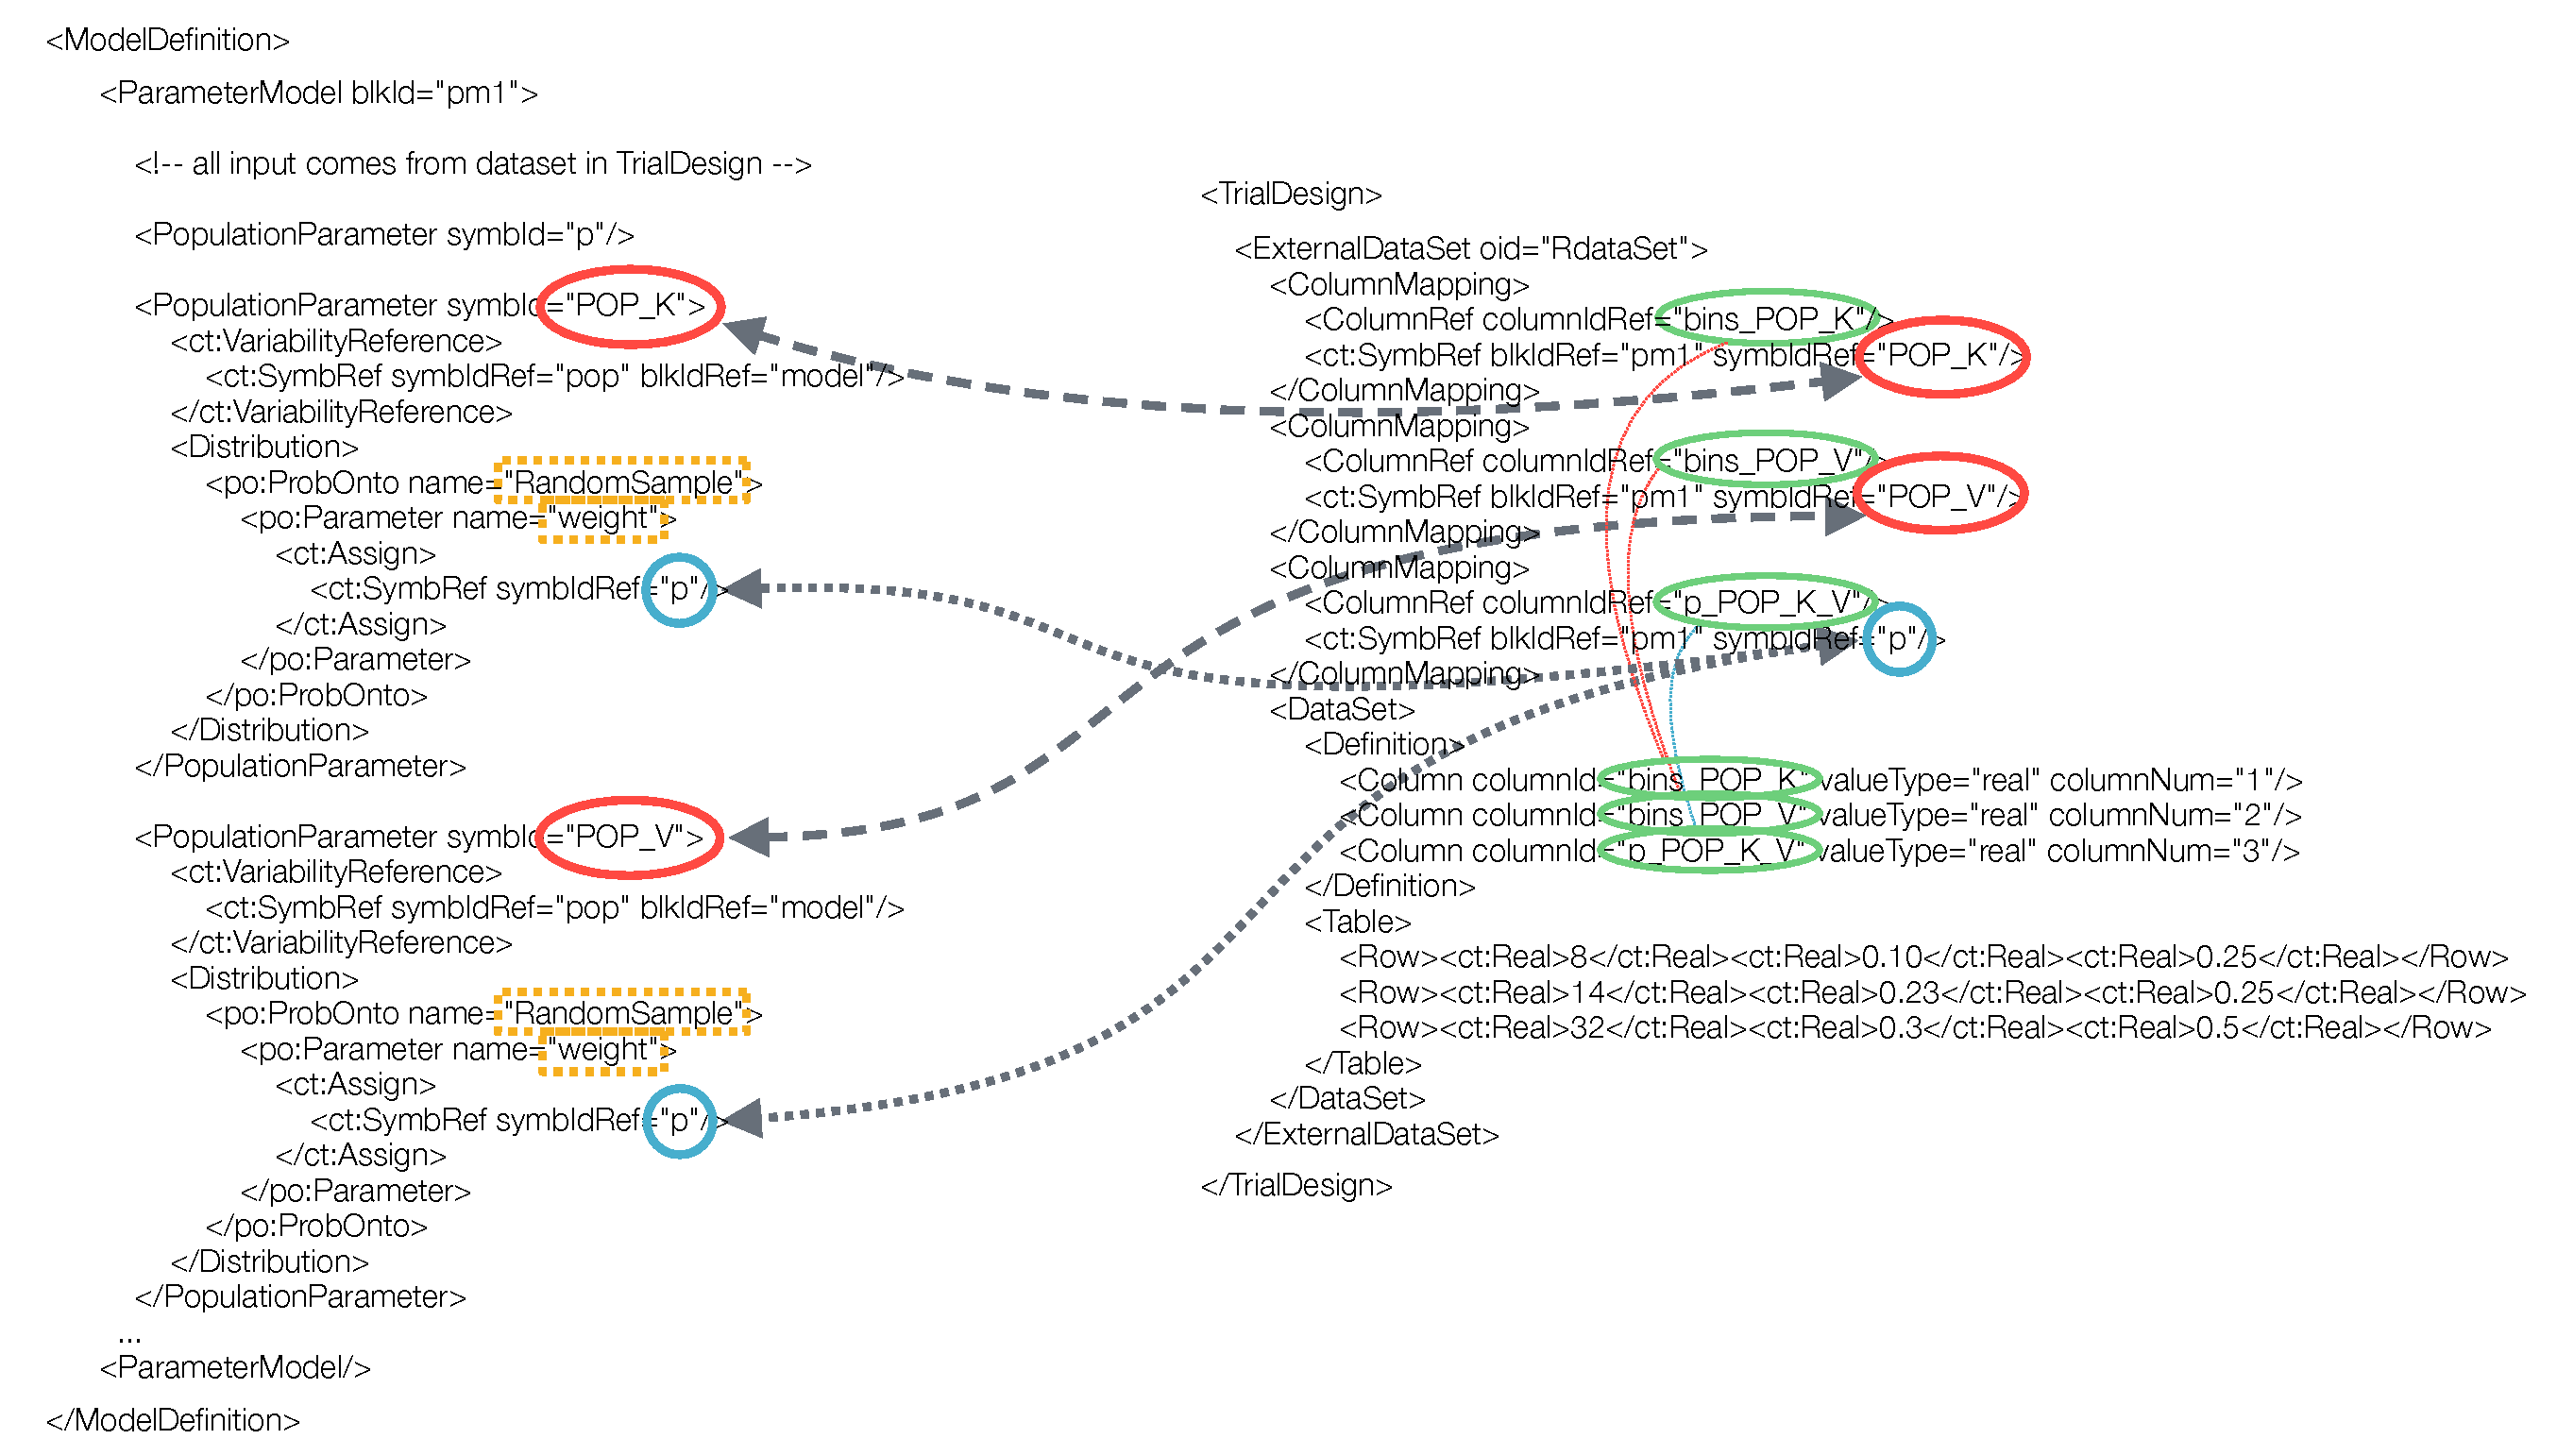
\includegraphics[width=180mm]{pics/Mapping_multiParams_withWeights.pdf}
 \caption{Mapping of samples with weights -- explained graphically.}
 \label{fig:Mapping_withWeights}
\end{figure}

PharmML implementation of the parameter model with distributions defined using
\emph{RandomSample} with \emph{weight} is as following

\lstset{language=XML}
\begin{lstlisting}
    <ParameterModel blkId="pm3">
        <PopulationParameter symbId="p"/>
        <PopulationParameter symbId="POP_K">
            <ct:VariabilityReference>
                <ct:SymbRef symbIdRef="pop" blkIdRef="vm1"/>
            </ct:VariabilityReference>
            <Distribution>
                <po:ProbOnto name="RandomSample">
                    <po:Parameter name="weight">
                        <ct:Assign>
                            <ct:SymbRef symbIdRef="p"/>
                        </ct:Assign>
                    </po:Parameter>
                </po:ProbOnto>
            </Distribution>
        </PopulationParameter>
        <PopulationParameter symbId="POP_V_sample">
            <ct:VariabilityReference>
                <ct:SymbRef symbIdRef="pop" blkIdRef="vm1"/>
            </ct:VariabilityReference>
            <Distribution>
                <po:ProbOnto name="RandomSample">
                    <po:Parameter name="weight">
                        <ct:Assign>
                            <ct:SymbRef symbIdRef="p"/>
                        </ct:Assign>
                    </po:Parameter>
                </po:ProbOnto>
            </Distribution>
        </PopulationParameter>
    </ParameterModel>
\end{lstlisting}
Then the dataset is defined in the \xelem{TrialDesign} as shown below
with the proper column mapping. 
\lstset{language=XML}
\begin{lstlisting}
    <TrialDesign>
        <ExternalDataSet oid="RdataSet">
            <ColumnMapping>
                <ds:ColumnRef columnIdRef="bins_POP_K"/>
                <ct:SymbRef blkIdRef="pm1" symbIdRef="POP_K"/>
            </ColumnMapping>
            <ColumnMapping>
                <ds:ColumnRef columnIdRef="bins_POP_V"/>
                <ct:SymbRef blkIdRef="pm1" symbIdRef="POP_V"/>
            </ColumnMapping>
            <ColumnMapping>
                <ds:ColumnRef columnIdRef="p_POP_V_K"/>
                <ct:SymbRef blkIdRef="pm1" symbIdRef="p"/>
            </ColumnMapping>
            <ds:DataSet>
                <ds:Definition>
                    <ds:Column columnId="bins_POP_K" valueType="real" columnNum="1"/>
                    <ds:Column columnId="bins_POP_V" valueType="real" columnNum="2"/>
                    <ds:Column columnId="p_POP_V_K" valueType="real" columnNum="3"/>
                </ds:Definition>
                <ds:Table>
                    <ds:Row><ct:Real>8</ct:Real><ct:Real>0.10</ct:Real><ct:Real>0.25</ct:Real></ds:Row>
                    <ds:Row><ct:Real>14</ct:Real><ct:Real>0.23</ct:Real><ct:Real>0.25</ct:Real></ds:Row>
                    <ds:Row><ct:Real>32</ct:Real><ct:Real>0.3</ct:Real><ct:Real>0.5</ct:Real></ds:Row>
                </ds:Table>
                <!--  <ds:ExternalFile oid="sxtData">
                        <ds:path>POP_V_K_sample.csv</ds:path>
                      </ds:ExternalFile>-->
            </ds:DataSet>
        </ExternalDataSet>
    </TrialDesign>
\end{lstlisting}



%%%%%%%%%%%%%%%%%%%%%%%%%%%%%%%%%%%%%%%%%%%%%%%%%%%%%%%
\subsection{Mapping using vectors}
\label{subsec:exp3}
(See the use case \emph{bayesianHierarchical/example3421dep\_NM.xml} using this option.)\\

In the case the modeller wants to encode a parameter in vector form, 
here $POP\_K$ and $POP\_V$ as vector elements  of $POP\_K\_V$ (see use cases 
in the \emph{bayesianHierarchical} example folder) there exist a possibility 
to map the vector to sample elements, see Figure 
\ref{fig:Mapping_multiParamsVectorised_withWeights} for a graphical 
explanation or the code snippet below.
% a declared of a vector is required first, e.g. $POP\_K\_V$ with subsequent declarations of 
%the single parameters defined using assignments such as $POP\_K = POP\_K\_V[1]$ 
%and $POP\_V = POP\_K\_V[2]$ -- this part is now shown in the PharmML code., 
%\marginpar{FINISH}
%The following series of code snippets shows how this 
%is done. First the declaration of $p\_POP\_K\_V$ and $POP\_K\_V$ is made
%\lstset{language=XML}
%\begin{lstlisting}
%            <PopulationParameter symbId="p_POP_K_V"/>
%            
%            <PopulationParameter symbId="POP_K_V">
%                <ct:VariabilityReference>
%                    <ct:SymbRef symbIdRef="pop" blkIdRef="model"/>
%                </ct:VariabilityReference>
%                <Distribution>
%                    <po:ProbOnto name="RandomSample">
%                        <po:Parameter name="weight">
%                            <ct:Assign>
%                                <ct:SymbRef symbIdRef="p_POP_K_V"/>
%                            </ct:Assign>
%                        </po:Parameter>
%                    </po:ProbOnto>
%                </Distribution>
%            </PopulationParameter>
%\end{lstlisting}
%and then $POP\_K = POP\_K\_V[1]$ assignment is encoded
%\lstset{language=XML}
%\begin{lstlisting}
%            <PopulationParameter symbId="POP_K">
%                <ct:Assign>
%                    <Uniop xmlns="http://www.pharmml.org/pharmml/0.7/Maths" op="exp">
%                        <ct:VectorSelector>
%                            <ct:SymbRef symbIdRef="POP_K_V"/>
%                            <ct:Cell>
%                                <ct:Int>1</ct:Int>
%                            </ct:Cell>
%                        </ct:VectorSelector>
%                    </Uniop>
%                </ct:Assign>
%            </PopulationParameter>
%\end{lstlisting}
%and analog for $POP\_V = POP\_K\_V[2]$ (not shown here).
\begin{figure}[ht!]
\centering
  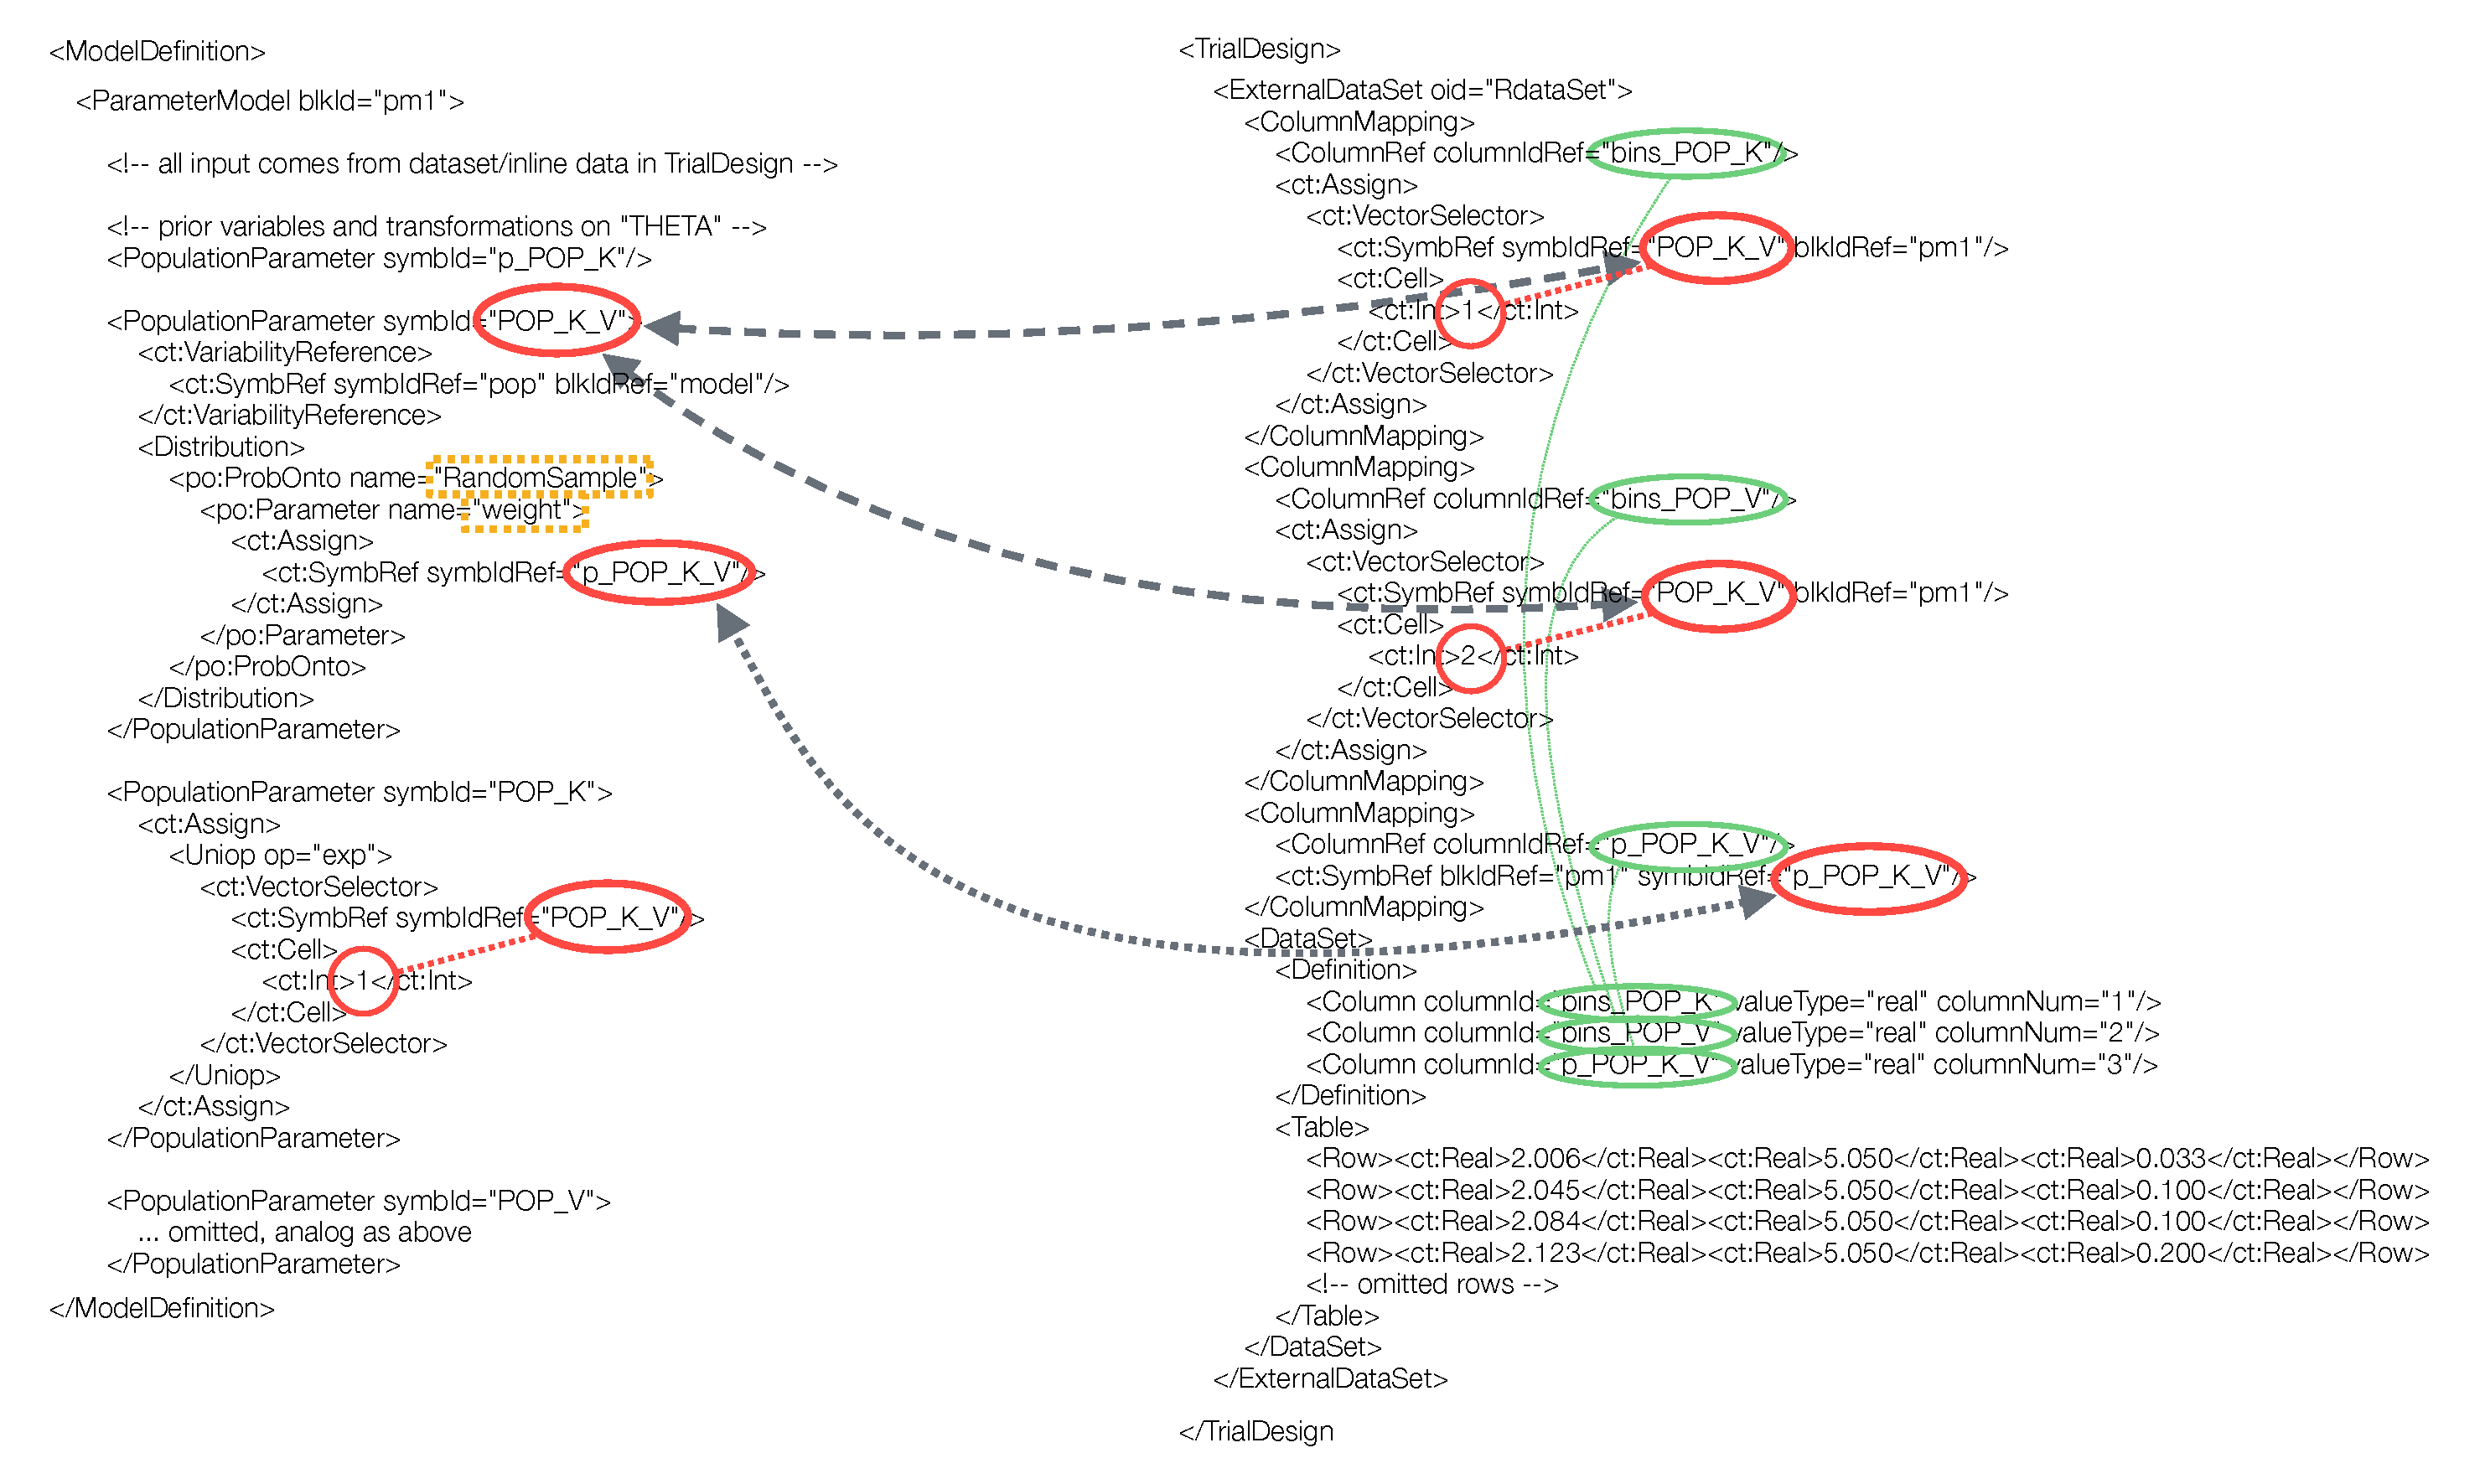
\includegraphics[width=180mm]{pics/Mapping_multiParamsVectorised_withWeights.pdf}
 \caption{Mapping of samples with vectors and weights -- explained graphically.}
 \label{fig:Mapping_multiParamsVectorised_withWeights}
\end{figure}

$POP\_K\_V$ is stored in dataset as $bins\_POP\_K$ in \xelem{TrialDesign} section and mapping between 
columns and model elements is performed using \xelem{ColumnMapping}
\lstset{language=XML}
\begin{lstlisting}
<ExternalDataSet oid="RdataSet">
    <ColumnMapping>
        <ColumnRef xmlns="http://www.pharmml.org/pharmml/0.7/Dataset" columnIdRef="bins_POP_K"/>
        <ct:Assign>
            <ct:VectorSelector>
                <ct:SymbRef symbIdRef="POP_K_V" blkIdRef="pm1"/>
                <ct:Cell>
                    <ct:Int>1</ct:Int>
                </ct:Cell>
            </ct:VectorSelector>
        </ct:Assign>
    </ColumnMapping>
    <ColumnMapping>
        <ColumnRef xmlns="http://www.pharmml.org/pharmml/0.7/Dataset" columnIdRef="bins_POP_V"/>
        <ct:Assign>
            <ct:VectorSelector>
                <ct:SymbRef symbIdRef="POP_K_V" blkIdRef="pm1"/>
                <ct:Cell>
                    <ct:Int>2</ct:Int>
                </ct:Cell>
            </ct:VectorSelector>
        </ct:Assign>
    </ColumnMapping>
    <ColumnMapping>
        <ColumnRef xmlns="http://www.pharmml.org/pharmml/0.7/Dataset" columnIdRef="p_POP_K_V"/>
        <ct:SymbRef symbIdRef="p_POP_K_V" blkIdRef="pm1"/>
    </ColumnMapping>
    <DataSet xmlns="http://www.pharmml.org/pharmml/0.7/Dataset">
        <Definition>
            <Column columnId="bins_POP_K" valueType="real" columnNum="1"/>
            <Column columnId="bins_POP_V" valueType="real" columnNum="2"/>
            <Column columnId="p_POP_K_V" valueType="real" columnNum="3"/>
        </Definition>
        <Table>
            <Row><ct:Real>2.006510</ct:Real><ct:Real>5.050013</ct:Real><ct:Real>0.033</ct:Real></Row>
            <Row><ct:Real>2.045465</ct:Real><ct:Real>5.050013</ct:Real><ct:Real>0.100</ct:Real></Row>
            <Row><ct:Real>2.084421</ct:Real><ct:Real>5.050013</ct:Real><ct:Real>0.100</ct:Real></Row>
            <Row><ct:Real>2.123377</ct:Real><ct:Real>5.050013</ct:Real><ct:Real>0.200</ct:Real></Row>
            <!-- rows skipped -->
        </Table>
    </DataSet>
</ExternalDataSet>
\end{lstlisting}

What is new in this version is the ability to map a particular vector element. Here the essential 
part is repeated to underline how the map of column \emph{bins\_POP\_V} and vector element
$POP\_K\_V[2]$ works.
\lstset{language=XML}
\begin{lstlisting}
    <ColumnMapping>
        <ColumnRef xmlns="http://www.pharmml.org/pharmml/0.7/Dataset" columnIdRef="bins_POP_V"/>
        <ct:Assign>
            <ct:VectorSelector>
                <ct:SymbRef symbIdRef="POP_K_V" blkIdRef="pm1"/>
                <ct:Cell>
                    <ct:Int>2</ct:Int>
                </ct:Cell>
            </ct:VectorSelector>
        </ct:Assign>
    </ColumnMapping>
\end{lstlisting}
See also Figure \ref{fig:Mapping_multiParamsVectorised_withWeights} which shows the mappings graphically.



%%%%%%%%%%%%%%%%%%%%%%%%%%%%%%%%%%%%%%%%%%%%%%%%%%%%%%%
\subsection{Samples in SO}
The concept of encoding samples of empirical distributions, either as inline tables of 
external dataset, is very useful also in the SO context, \cite{SO:2015}. 
For example the posterior distribution of individual parameters estimates is captured 
using an empirical distribution, \emph{RandomSample}.
Here the values for three estimated parameters are encoded inline.
\lstset{language=XML}
\begin{lstlisting}
    <PosteriorDistribution>
        <Distribution>
            <po:ProbOnto name="RandomSample">
                <ds:DataSet>
                    <ds:Definition>
                        <ds:Column columnId="K" columnType="popParameter" valueType="real" columnNum="1"/>
                        <ds:Column columnId="V" columnType="popParameter" valueType="real" columnNum="2"/>
                        <ds:Column columnId="CL" columnType="popParameter" valueType="real" columnNum="3"/>
                    </ds:Definition>
                    <ds:Table>
                        <ds:Row><ct:Real>2.006510</ct:Real><ct:Real>5.050013</ct:Real><ct:Real>0.033333</ct:Real></ds:Row>
                        <ds:Row><ct:Real>2.045465</ct:Real><ct:Real>5.050013</ct:Real><ct:Real>0.100000</ct:Real></ds:Row>
                        <ds:Row><ct:Real>2.084421</ct:Real><ct:Real>5.050013</ct:Real><ct:Real>0.100000</ct:Real></ds:Row>
                        <ds:Row><ct:Real>2.123377</ct:Real><ct:Real>5.050013</ct:Real><ct:Real>0.200000</ct:Real></ds:Row>
                        <ds:Row><ct:Real>2.162333</ct:Real><ct:Real>5.064166</ct:Real><ct:Real>0.100000</ct:Real></ds:Row>
                        <ds:Row><ct:Real>2.201288</ct:Real><ct:Real>5.064166</ct:Real><ct:Real>0.066667</ct:Real></ds:Row>
                        <!-- other sample rows skipped -->
                    </ds:Table>
                    <!-- 
                        <ds:ExternalFile oid="extDataId">
                            <ds:path>samples_KVCL.csv</ds:path>
                        </ds:ExternalFile>-->
                </ds:DataSet>
            </po:ProbOnto>
        </Distribution>
    </PosteriorDistribution>
 \end{lstlisting}
The alternative using external datasets is commented out. Note also that no mapping 
is required in this case, the symbol assigned to the attribute \xatt{columnId} 
identifies the parameter.


%%%%%%%%%%%%%%%%%%%%%%%%%%%%%%%%%%%%%%%%%%%%%%%%%%%%%%%
\section{Random realisations}
\label{sec:randRealisations}
Another new feature in version 0.8 is the possibility to specify a single realisation from any
univariate distribution and is based on analogue featured in UncertML, 
\cite{uncertml3:2014}. The definition reads:
\begin{description}
\item[Realisation] is a single instance of a random variable and can be used 
to imply an observed value, or, as more widely used, a single draw, $x_i$, from a 
probability distribution, $p(x)$.
\end{description}

A new element \xelem{Realisation} has been introduced referring to ProbOnto 
with the specification of the code name of the distribution of interest and its parameters 
as the following example shows.

\subsubsection*{Example}
Source \cite{MLXTRANforSimulator:2014}. Categorical covariates can be defined 
as a discrete transformation of continuous random variables. Consider for instance the following 
model encoded in MLXTRAN.
 
\lstset{language=MLX}
\begin{lstlisting}
	[COVARIATE]
	DEFINITION:
	z = {distribution=normal, mean=0, sd=1}
	
	EQUATION:
	if z<-0.2533 ; P(z<-0.2533)=0.4
		cz = 0
	else
		cz = 1
	end
	c=cz
\end{lstlisting}
Note, that \xatt{z=\{distribution=normal,...\}} in the \xatt{DEFINITION} block is a sampling
assignment which is encoded in the element \xelem{Realisation}.
\lstset{language=MLX}
\begin{lstlisting}
        <CovariateModel blkId="cm2">
            <Covariate symbId="z">
                <Continuous>
                    <Realisation>
                        <po:ProbOnto name="StandardNormal1"/>
                    </Realisation>
                </Continuous>
            </Covariate>
\end{lstlisting}
The remaining definition and assignment of a new covariate is conditional 
on the sampled value \emph{z}
\lstset{language=MLX}
\begin{lstlisting}
            <Covariate symbId="cz">
                <Categorical>
                    <ct:Assign>
                        <ct:Piecewise>
                            <math:Piece>
                                <ct:Real>0</ct:Real>
                                <math:Condition>
                                    <math:LogicBinop op="lt">
                                        <ct:SymbRef symbIdRef="z"/>
                                        <ct:Real>-0.2533</ct:Real>
                                    </math:LogicBinop>
                                </math:Condition>
                            </math:Piece>
                            <math:Piece>
                                <ct:Real>1</ct:Real>
                                <math:Condition>
                                    <math:Otherwise/>
                                </math:Condition>
                            </math:Piece>
                        </ct:Piecewise>
                    </ct:Assign>
                </Categorical>
            </Covariate>
        </CovariateModel>
\end{lstlisting}


%%%%%%%%%%%%%%%%%%%%%%%%%%%%%%%%%%%%%%%%%%%%%%%%%%%%%%%
\section{Markov models}
\label{sec:MM}
New element -- transition aka stochastic matrix -- has been introduced to simplify encoding of Markov models. 
\subsection{Transition matrix}
\label{sec:transitionMatrix}
Stochastic (aka transition matrix) is a matrix used to describe the transitions in a Markov 
chain\footnote{\url{https://en.wikipedia.org/wiki/Stochastic_matrix}}. A stochastic matrix can be 
characterised further by the optional attribute 
\begin{itemize}
\item
Left stochastic (default), \xatt{type="leftStochastic"}, a real square matrix, with each row summing to 1.
\item
Right stochastic, \xatt{type="rightStochastic"},  a real square matrix, with each column summing to 1.
\item
Doubly stochastic, \xatt{type="doubleStochastic"},  both columns and rows are summing to 1.
\end{itemize}
Figure \ref{fig:transitionMatrix} visualises a basic Markov model with the according transition 
matrix and the XML code shows how it is implemented 
\begin{figure}[ht!]
\centering
  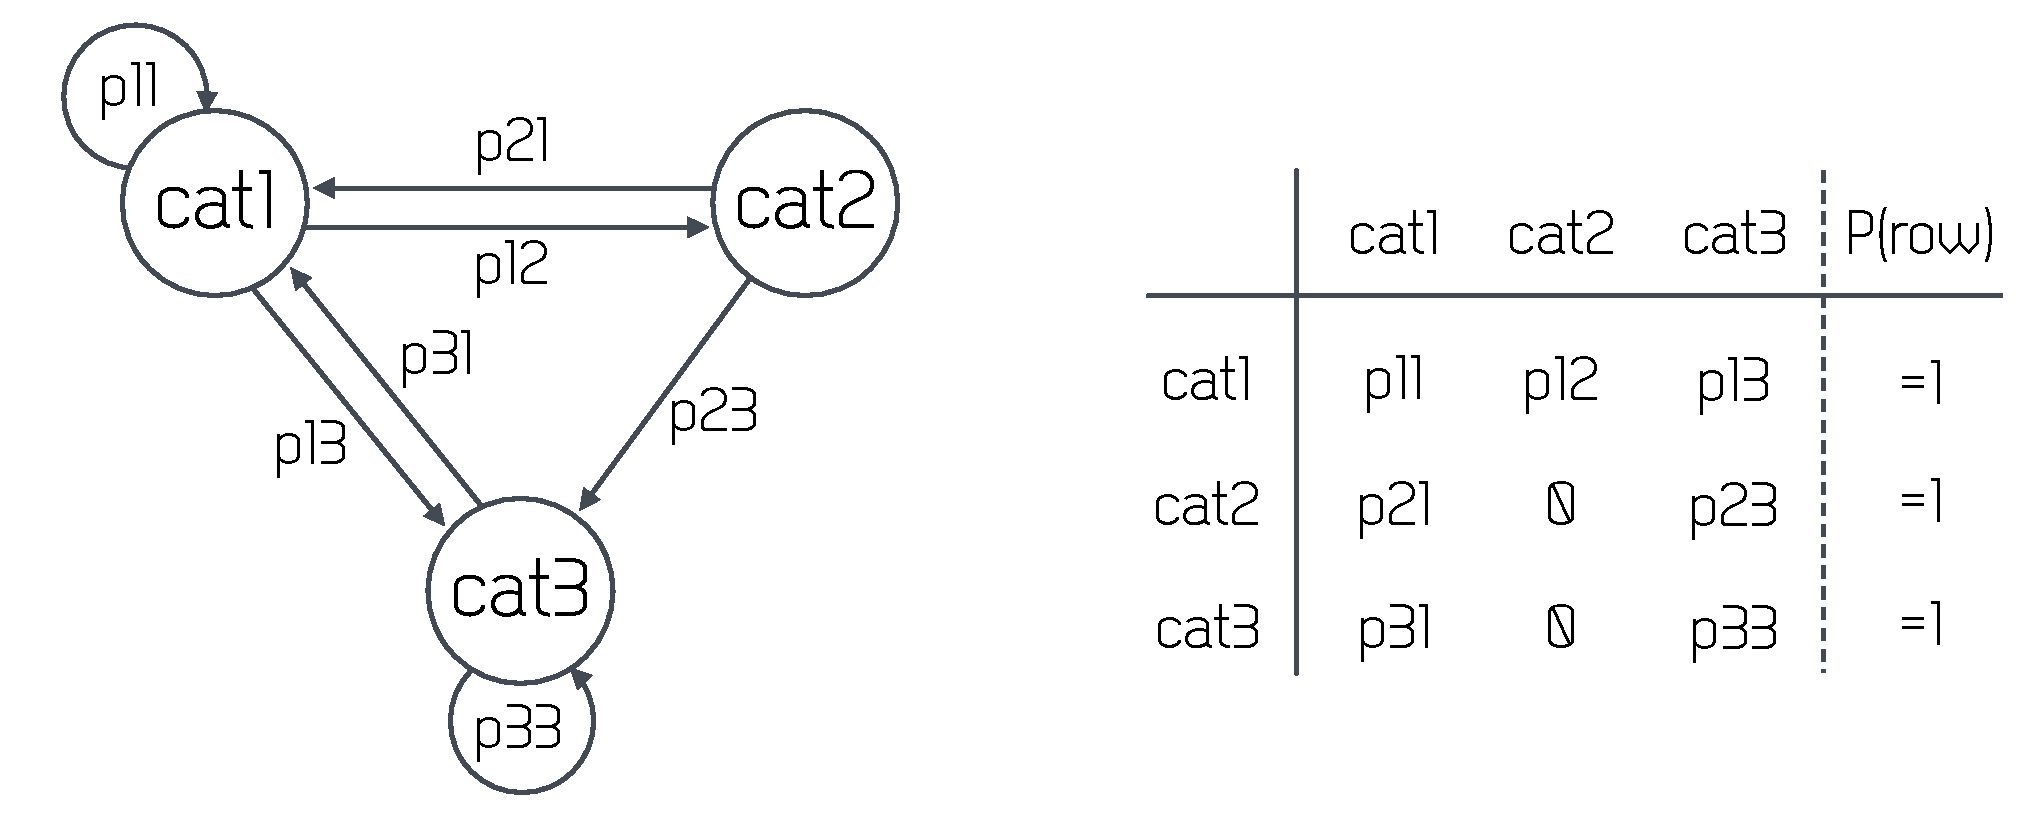
\includegraphics[width=125mm]{pics/transitionMatrix.pdf}
 \caption{An example for a transition matrix for a Markov chain. 
 (Left) the state transition diagram with three possible 
 states cat1, cat2, and cat3. (Right) the \textbf{left} transition matrix.}
 \label{fig:transitionMatrix}
\end{figure}
\lstset{language=XML}
\begin{lstlisting}
        <Dependance type="discreteMarkov"/>
        <TransitionMatrix type="leftStochastic">
            <ct:Matrix matrixType="Any">
                <ct:ColumnNames>
                    <ct:SymbRef symbIdRef="cat1"/>
                    <ct:SymbRef symbIdRef="cat2"/>
                    <ct:SymbRef symbIdRef="cat3"/>
                </ct:ColumnNames>
                <ct:MatrixRow>
                    <ct:SymbRef symbIdRef="p11"/>
                    <ct:SymbRef symbIdRef="p12"/>
                    <ct:SymbRef symbIdRef="p13"/>
                </ct:MatrixRow>
                <ct:MatrixRow>
                    <ct:SymbRef symbIdRef="p21"/>
                    <ct:Real>0</ct:Real>
                    <ct:SymbRef symbIdRef="p23"/>
                </ct:MatrixRow>
                <ct:MatrixRow>
                    <ct:SymbRef symbIdRef="p31"/>
                    <ct:Real>0</ct:Real>
                    <ct:SymbRef symbIdRef="p33"/>
                </ct:MatrixRow>
            </ct:Matrix>
        </TransitionMatrix>
\end{lstlisting}
If the \xatt{type} attribute is not used, the default is the \xatt{leftStochastic} matrix.

\begin{figure}[ht!]
\centering
  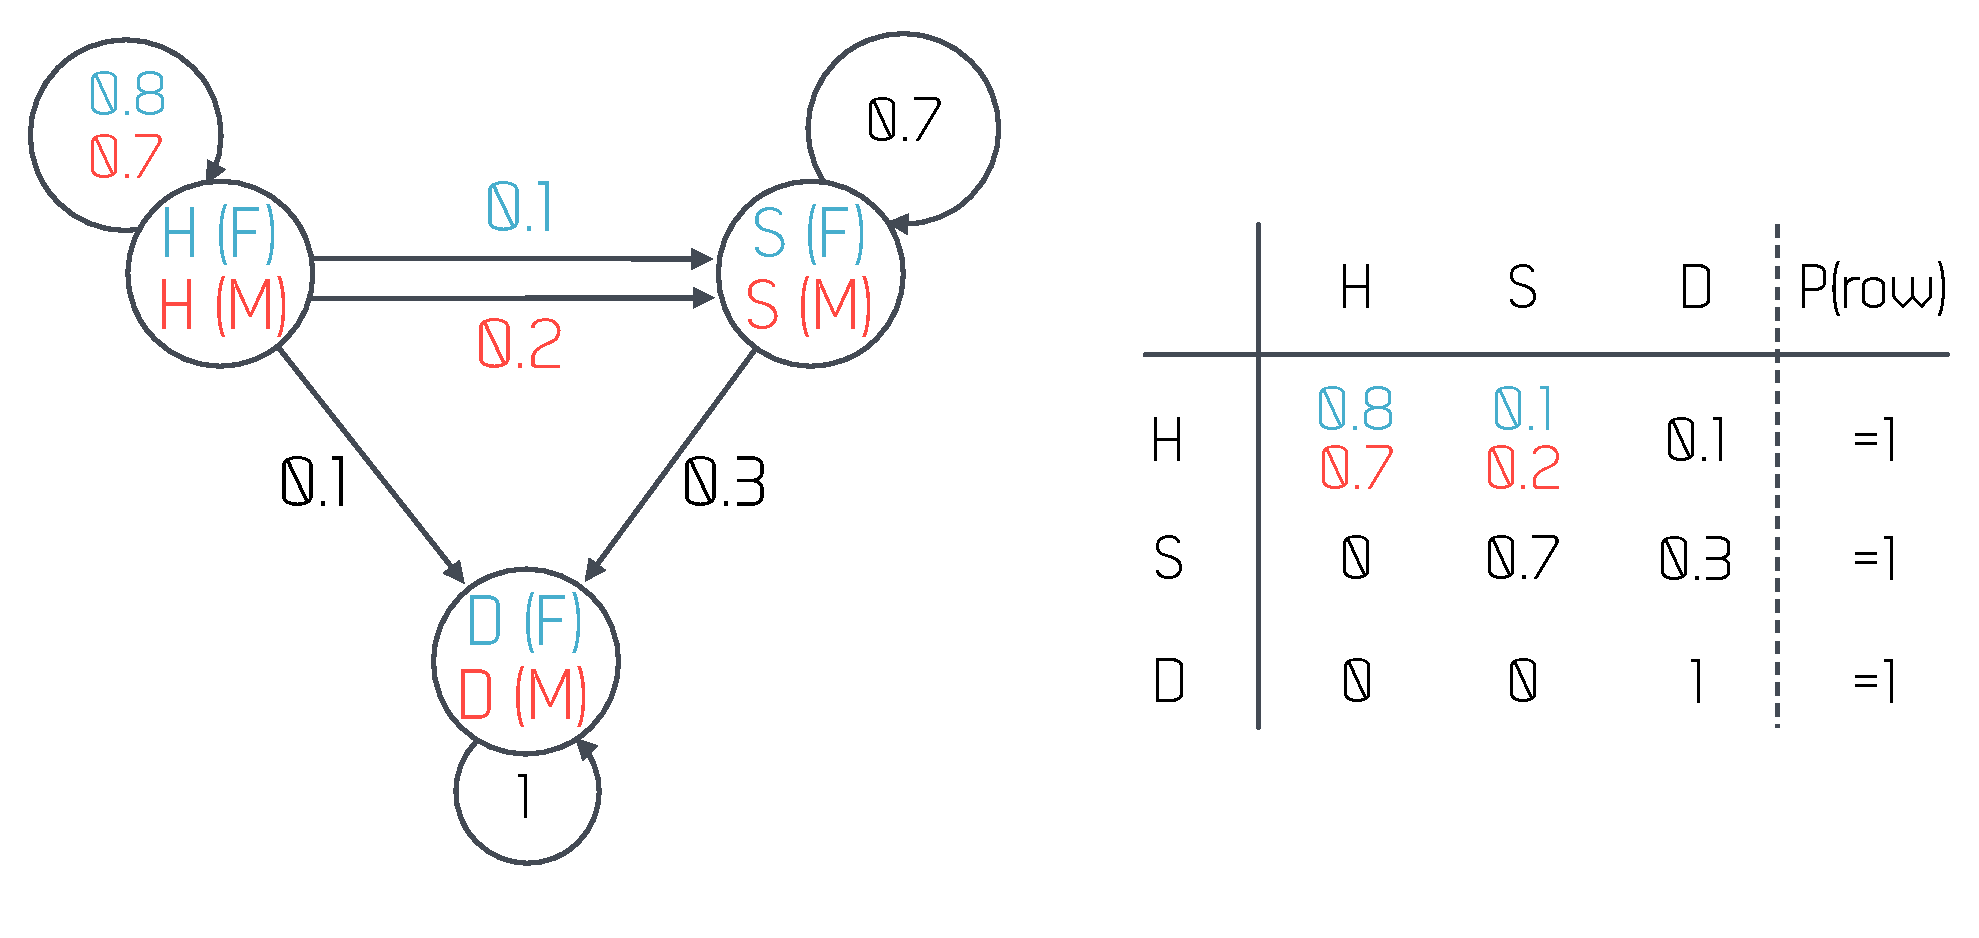
\includegraphics[width=120mm]{pics/markovMatrixCond.pdf}
 \caption{An example of a conditional Markov model with the according transition matrix.
 It is a left stochastic matrix with probabilities in each raw summing up to 1.}
 \label{fig:markovMatrixCond}
\end{figure}


\subsection{Conditional transition probabilities/matrix}
\label{sec:condTransitionMatrix}
Conditional transition probabilities can be implemented pairwise, e.g.
\begin{align}
& P(\mbox{Cat1} \rightarrow \mbox{Cat2} | \; \mbox{COLOR}==\mbox{BLUE}) = p12_{BLUE} \nonumber \\
& P(\mbox{Cat1} \rightarrow \mbox{Cat2} | \; \mbox{COLOR}==\mbox{RED}) = p12_{RED} \nonumber \\
& \mbox{other probabilities omitted...} \nonumber
\end{align}
or with a conditional transition matrix using piecewise statements were required, 
Figure \ref{fig:markovMatrixCond}. See also section \ref{sec:markovModels} for use examples.


%\subsection{Encoding Markov models -- question}
%Markov models are right now encode as categorical ones. The 

%%%%%%%%%%%%%%%%%%%%%%%%%%%%%%%%%%%%%%%%%%%%%%%%%%%%%%%
\section{N-ary operators}
\label{sec:NaryOps}
N-ary operators are an extension of binary operators in cases when
more then two arguments are provided. The current version supports the 
following operators
%\begin{itemize}
%\item 
%\xatt{plus} - addition operator for n arguments 
%\item 
%\xatt{times} - multiplication operator for n arguments 
%\item 
%\xatt{min} -- minimum of n arguments
%\item 
%\xatt{max} -- maximum of n arguments
%\item 
%\xatt{gcd} -- greatest common divisor of its arguments
%\item 
%\xatt{lcm} -- least common multiple of its arguments
%\end{itemize}

\begin{longtable}{llcc}
\hline
\hline
\textbf{N-ary operator}		& \textbf{Name}	& \textbf{Argument 1 ... N}& \textbf{Return type}\\
\hline
Addition					& \xatt{plus}		& \xatt{X}, ..., \xatt{X}	& \xatt{Real} \\
Multiplication				& \xatt{times}		& \xatt{X}, ..., \xatt{X}	& \xatt{Real} \\
Smallest of the arguments	& \xatt{min}		& \xatt{X}, ..., \xatt{X}	& \xatt{Real} \\
Largest of the arguments		& \xatt{max}		& \xatt{X}, ..., \xatt{X}	& \xatt{Real} \\
Greatest common divisor		& \xatt{gcd}		& \xatt{X}, ..., \xatt{X}	& \xatt{Real} \\
Least common multiple		& \xatt{lcm}		& \xatt{X}, ..., \xatt{X}	& \xatt{Real} \\
\hline
\caption{N-ary operators supported in v0.8.}
\label{tab:naryops}
\end{longtable}%


\subsection{Rules for using \xelem{Naryop}}

\begin{itemize}
\item 
\xatt{X} can be either a variable reference, real vector, vector/matrix (if a raw/column is
required) selector or sequence.
\item
when more then one argument is required \xelem{Vector} with \xelem{VectorElements} has to be used.
%\item 
%or \xelem{VectorSelector}  can be used
%\end{itemize}
\end{itemize}

\subsubsection*{Example}
An example of the use of N-ary operators is shown below using the
\xatt{max} operator applied to a vector of numbers
and symbol references, e.g. Amax = max(1, a2, 3, a4, fifthElement, $\dots$).
\lstset{language=XML}
\begin{lstlisting}
            <IndividualParameter symbId="Amax">
                <ct:Assign>
                    <math:Naryop op="max">
                        <ct:Vector>
                            <ct:VectorElements>
                                <ct:Real>1</ct:Real>
                                <ct:SymbRef symbIdRef="a2"/>
                                <ct:Real>3</ct:Real>
                                <ct:SymbRef symbIdRef="a4"/>
                                <ct:SymbRef symbIdRef="fifthElement"/>
                                <!-- ... -->
                            </ct:VectorElements>
                        </ct:Vector>
                    </math:Naryop>
                </ct:Assign>
            </IndividualParameter>
\end{lstlisting}


%%%%%%%%%%%%%%%%%%%%%%%%%%%%%%%%%%%%%%%%%%%%%%%%%%%%%%%
\section{Statistical operators}
\label{sec:statsOps}
Based on the UncertML collection, a set of basic statistics is supported in v0.8 
as shown in Table \ref{tab:statistics}. Arguments X and Y can be references 
to variables or explicit vectors of values, see examples below. In few cases 
a second argument is required, \emph{level} or \emph{order}. The order of the 
arguments, 'Argument 2' must follow 'Argument 1', is important as it determines 
the meaning of the argument.
\begin{longtable}{llccc}
\hline
\hline
\textbf{Statistic}		& \textbf{Name}			& \textbf{1$^{st}$argument} 	& \textbf{2$^{nd}$argument} 	& \textbf{Return type}\\
\hline
Centred moment	& \xatt{centredMoment}		& \xatt{X}		& \xatt{order} $\in \mathbb N$	& \xatt{Real} \\
Coeff. of variation	& \xatt{coefficientOfVariation}	& \xatt{X} 		& -- 						& \xatt{Real} \\
Correlation		& \xatt{correlation}			& \xatt{X} 		& \xatt{Y}  				& \xatt{Real} \\
Decile			& \xatt{decile}				& \xatt{X} 		& \xatt{level} $\in \{1,..., 9\}$ 	& \xatt{Real} \\
Geometric mean	& \xatt{geometricMean}		& \xatt{X} 		& -- 						& \xatt{Real} \\
Kurtosis			& \xatt{kurtosis}			& \xatt{X} 		& -- 						& \xatt{Real} \\
Mean			& \xatt{mean}				& \xatt{X} 		& -- 						& \xatt{Real} \\
Median			& \xatt{median}				& \xatt{X} 		& -- 						& \xatt{Real} \\
Mode			& \xatt{mode}				& \xatt{X} 		& -- 						& \xatt{Real} \\
Moment			& \xatt{moment}			& \xatt{X} 		& \xatt{order} $\in \mathbb N$ 	& \xatt{Real} \\
Percentile			& \xatt{percentile}			& \xatt{X} 		& \xatt{level} $\in$ [0, 100]	& \xatt{Real} \\
Quantile			& \xatt{quantile}			& \xatt{X} 		& \xatt{level} $\in$ [0, 1] 		& \xatt{Real} \\
Quartile			& \xatt{quartile}				& \xatt{X} 		& \xatt{level} $\in \{0.25, 0.5, 0.75, 1\}$ 	& \xatt{Real} \\
Range			& \xatt{range}				& \xatt{X} 		& -- 						& \xatt{Real} \\
Skewness			& \xatt{skewness}			& \xatt{X} 		& -- 						& \xatt{Real} \\
Stand. deviation	& \xatt{standardDeviation}	& \xatt{X} 		& -- 						& \xatt{Real} \\
Variance			& \xatt{variance}			& \xatt{X} 		& -- 						& \xatt{Real} \\
\hline
\caption{Statistics supported in v0.8. The type of the arguments \xatt{X} and \xatt{Y} 
can be either variable references or real vectors. Multiple values 
without \xelem{Vector} element are not allowed. In few cases a second argument 
is required, \xatt{level} or \xatt{order}. The correct sequence of the arguments, 
first 'Argument 1' then 'Argument 2', is important as it determines the meaning 
of the arguments.}
\label{tab:statistics}
\end{longtable}%

\subsection{Rules for using \xelem{Statsop}}
\begin{itemize}
\item
arguments \xatt{X} and \xatt{Y} can be either variable references or real vectors
\item
type of arguments \xatt{level} and \xatt{order} is specified in the Table \ref{tab:statistics}
\item 
only two arguments are allowed as children of \xelem{Statsop}, see Table \ref{tab:statistics}
\item 
for statistics where more then two arguments are expected, \xelem{Vector}
with \xelem{VectorElements} has to be used.
\end{itemize}

\subsection{Examples}
Some examples of the use of statistical operators are shown below. 
\subsubsection*{Basic example}
This example shows how to use the \emph{mean} operator acting on
existing parameters
\lstset{language=XML}
\begin{lstlisting}
            <PopulationParameter symbId="Qm">
                <ct:Assign>
                    <math:Statsop op="mean">
                        <ct:Vector>
                            <ct:VectorElements>
                                <ct:SymbRef blkIdRef="pm1" symbIdRef="Q0"/>
                                <ct:SymbRef blkIdRef="pm1" symbIdRef="Q1"/>
                                <ct:SymbRef blkIdRef="pm1" symbIdRef="Q2"/>
                            </ct:VectorElements>
                        </ct:Vector>
                    </math:Statsop>	
                </ct:Assign>
            </PopulationParameter>
\end{lstlisting}

\subsubsection*{More example}
The next few examples show how to use these operators given a dummy dataset for 
which a histogram and a box plot has been plotted in Figure \ref{fig:quantiles}.  
\begin{figure}[ht!]
\centering
  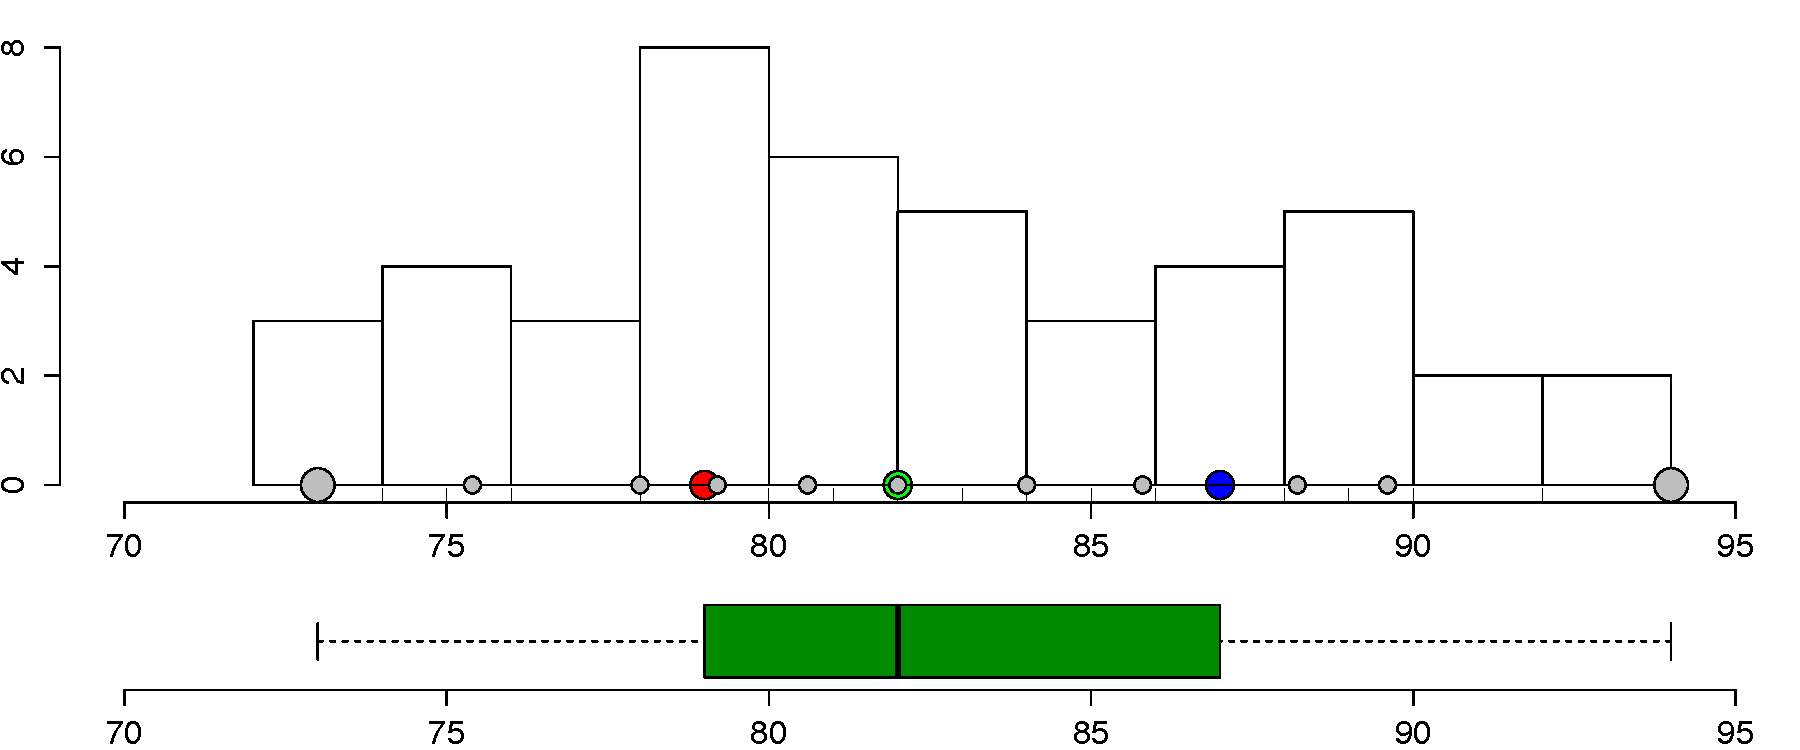
\includegraphics[width=160mm]{pics/quantiles.pdf}
 \caption{Deciles (grey), quartiles: 1$^{st}$ (red), 2$^{nd}$/median (green) and 3$^{rd}$ 
 (blue) and min/max (large grey circles). Any of these characteristic points can be specified now in PharmML
 for a given dataset or random variable using either the statistical or n-ary operators.}
 \label{fig:quantiles}
\end{figure}
The dataset \xatt{scores = [78, 84, 83, ..., 81, 92, 89]}\footnote{The whole set is: [78, 84, 83, 80, 94, 90, 81, 79, 79, 81, 85, 87, 86, 89, 92, 78, 74, 83, 80, 74, 80, 82, 89, 89, 73, 75, 87, 76, 79, 84, 78, 76, 75, 85, 79, 82, 87, 84, 94, 88, 80, 82, 81, 92, 89]} can be imagined being mapped from an external file or 
a non-parametric distribution using the sample concept, see section \ref{sec:nonParamDistribs},
here with inline encoded data 
\lstset{language=XML}
\begin{lstlisting}
            <PopulationParameter symbId="scores">
                <Distribution>
                    <po:ProbOnto name="RandomSample">
                        <ds:DataSet>
                            <ds:Table>
                                <!-- 78, 84, 83, ..., 81, 92, 89 -->
                                <ds:Row>
                                    <ct:Real>78</ct:Real><ct:Real>84</ct:Real><ct:Real>83</ct:Real>
                                    <!-- omitted values -->
                                    <ct:Real>81</ct:Real><ct:Real>92</ct:Real><ct:Real>89</ct:Real>
                                </ds:Row>
                            </ds:Table>
                        </ds:DataSet>
                    </po:ProbOnto>
                </Distribution>
            </PopulationParameter>
\end{lstlisting}

The typical numbers characterising this sample, such as deciles or quartiles, can be
defined in PharmML as the following snippets show
\begin{itemize}
\item 
Q1 -- 1$^{st}$ quartile (red dot in Figure \ref{fig:quantiles})
\lstset{language=XML}
\begin{lstlisting}
            <PopulationParameter symbId="Q1">
                <ct:Assign>
                    <math:Statsop op="quartile">
                        <ct:SymbRef symbIdRef="scores"/>
                        <ct:Real>0.25</ct:Real>
                    </math:Statsop>
                </ct:Assign>
            </PopulationParameter>
\end{lstlisting}
\item 
Median/Q2 -- median / 2$^{nd}$ quartile (green)
\lstset{language=XML}
\begin{lstlisting}
            <PopulationParameter symbId="Median">
                <ct:Assign>
                    <math:Statsop op="median">
                        <ct:SymbRef symbIdRef="scores"/>
                    </math:Statsop>
                </ct:Assign>
            </PopulationParameter>
            
            <PopulationParameter symbId="Q2">
                <ct:Assign>
                    <math:Statsop op="quartile">
                        <ct:SymbRef symbIdRef="scores"/>
                        <ct:Real>0.5</ct:Real>
                    </math:Statsop>
                </ct:Assign>
            </PopulationParameter>
\end{lstlisting}
\item 
Q3 -- 3$^{rd}$ quartile (blue)
\lstset{language=XML}
\begin{lstlisting}
            <PopulationParameter symbId="Q3">
                <ct:Assign>
                    <math:Statsop op="quartile">
                        <ct:SymbRef symbIdRef="scores"/>
                        <ct:Real>0.75</ct:Real>
                    </math:Statsop>
                </ct:Assign>
            </PopulationParameter>
\end{lstlisting}
\item 
D5 -- 4$^{th}$ decile (gray)
\lstset{language=XML}
\begin{lstlisting}
            <PopulationParameter symbId="D4">
                <ct:Assign>
                    <math:Statsop op="decile">
                        <ct:SymbRef symbIdRef="scores"/>
                        <ct:Int>4</ct:Int>
                    </math:Statsop>
                </ct:Assign>
            </PopulationParameter>
\end{lstlisting}
\end{itemize}


\section{Covariates versus regressors}
\label{sec:covVsRegs}
There is no unified naming convention for covariates and regressors
and we assume the following classification based on the DDMoRe discussions and
target tool related literature, \cite{NONMEM:2009} and \cite{LavielleBook:2014},
\begin{itemize}
\item 
constant covariates
\item 
occasion dependent covariates
\item 
time dependent covariates -- \emph{aka} regressors 
\end{itemize}
Due to the various interpretation and nomenclature there is a need to identify 
those and this can be done also in the \xelem{CovariateModel} by assigning an optional attribute
\xatt{type} with values \emph{occasionDependent}, \emph{timeDependent}, 
\emph{constant}. The following snippet shows how this is done for 
a occasion dependent covariate 

\lstset{language=XML}
\begin{lstlisting}
        <CovariateModel blkId="cm1">
            <Covariate type="occasionDependent" symbId="CovariateX">
                <!-- ... -->
            </Covariate>
        </CovariateModel>
\end{lstlisting}
For more on regressor support in PharmML, see Section "6.4 Regressor support"
in v0.7 spec \cite{Swat:2015b}.


%%%%%%%%%%%%%%%%%%%%%%%%%%%%%%%%%%%%%%%%%%%%%%%%%%%%%%%
\section{Extension in categorical covariate model}
\label{sec:catCovModel}
Until now the only option for categorical covariates was to declare them
with their categories and (if required) associated probabilities. Version 0.8
comes few a number of extensions.

\subsection{Covariate declaration/assignment}
Declaration of new categorical covariates, based on existing ones,
is now possible. Here a simple example of a conditional definition from one of the IOG use cases
\lstset{language=NM}
\begin{lstlisting}
            DDU = if (DDUR > 2) then 1 # duration > 1 month
            else 0 # duration of current episode < 1 month
\end{lstlisting}
which implementation in XML using the piecewise structure reads
\lstset{language=XML}
\begin{lstlisting}
    <Covariate symbId="DDU">
        <Categorical>
            <ct:Assign>
                <ct:Piecewise>
                    <math:Piece>
                        <ct:Real>1</ct:Real>
                        <math:Condition>
                            <math:LogicBinop op="lt">
                                <ct:SymbRef symbIdRef="DDUR"/>
                                <ct:Real>2</ct:Real>
                            </math:LogicBinop>
                        </math:Condition>
                    </math:Piece>
                    <math:Piece>
                        <ct:Real>0</ct:Real>
                        <math:Condition>
                            <math:Otherwise/>
                        </math:Condition>
                    </math:Piece>
                </ct:Piecewise>
            </ct:Assign>
        </Categorical>
    </Covariate>
\end{lstlisting}


\subsection{Unified distribution definition}

The possibility to define distribution of categorical covariates was given 
before but was inconsistent with the way continuous covariates are handled.
While the previous option (using \xelem{Probability} for each category is still
supported), the \xelem{Distribution} element referring to any ProbOnto distribution 
can be used now as well.

\begin{longtable}{cc}
\hline
\hline
option supported in $\le$ 0.7.3 & new option in version 0.8 \\
\hline
\lstset{language=XML}
\begin{lstlisting}
<Covariate symbId="Sex">
    <Categorical>
        <Category catId="F">
            <Probability>
                <ct:SymbRef symbIdRef="p1"/>
            </Probability>
        </Category>
        <Category catId="M">
            <Probability>
                <ct:SymbRef symbIdRef="p2"/>
            </Probability>
        </Category>
    </Categorical>
</Covariate>
\end{lstlisting}
&
\lstset{language=XML}
\begin{lstlisting}
<Covariate symbId="Sex">
    <Categorical>
        <Category catId="F"/>
        <Category catId="M"/>
        <Distribution>
            <po:ProbOnto name="CategoricalNonordered1">
                <po:Parameter name="categoryProb">
                    <ct:Assign>
                        <ct:Vector>
                            <ct:VectorElements>
                                <ct:SymbRef symbIdRef="p1"/>
                                <ct:SymbRef symbIdRef="p2"/>
                            </ct:VectorElements>
                        </ct:Vector>
                    </ct:Assign>
                </po:Parameter>
            </po:ProbOnto>
        </Distribution>
    </Categorical>
</Covariate>
\end{lstlisting}
\\
\hline
\caption{Declaration of categorical covariates distribution using \xelem{Distribution} and 
\xelem{ProbOnto} elements in now supported (right).}
\label{tab:catCovDistrib}
\end{longtable}%

\subsection{Conditional distributions}
Also new is the possibility to define a conditional covariate distribution.
E.g. the previous example in Table \ref{tab:catCovDistrib} is extended in that the 
SEX distribution varies between studies, with probabilities given by the two following 
vectors $\boldsymbol {p_{S1}} = \{p1_{S1},p2_{S1}\}$ or $\boldsymbol {p_{S2}} = \{p1_{S2},p2_{S2}\}$.
Such model reads then 
\bigskip
\begin{algorithmic}
	\If {$STUDY == S1$}
	    \State SEX $\sim$ Categorical($\boldsymbol {p_{S1}}$)
	\ElsIf{$STUDY == S2$} 
	    \State SEX $\sim$ Categorical($\boldsymbol {p_{S2}}$)
	\EndIf
\end{algorithmic}
\bigskip
First the STUDY  covariate is declared with category identifiers S1 and S2
\lstset{language=XML}
\begin{lstlisting}
            <Covariate symbId="STUDY">
                <Categorical>
                    <Category catId="S1"/>
                    <Category catId="S2"/>
                </Categorical>
            </Covariate>
\end{lstlisting}
then the distribution of SEX can be defined using here the \emph{CategoricalNonordered1} 
distribution defined in ProbOnto 
\lstset{language=XML}
\begin{lstlisting}
            <Covariate symbId="SEX">
                <Categorical>
                    <Category catId="F"/>
                    <Category catId="M"/>
                    <Distribution>
                        <Piecewise>
                            <math:Piece>
                                <po:ProbOnto name="CategoricalNonordered1">
                                    <po:Parameter name="categoryProb">
                                        <ct:Assign>
                                            <ct:Vector>
                                                <ct:VectorElements>
                                                    <ct:SymbRef symbIdRef="p1_S1"/>
                                                    <ct:SymbRef symbIdRef="p2_S1"/>
                                                </ct:VectorElements>
                                            </ct:Vector>
                                        </ct:Assign>
                                    </po:Parameter>
                                </po:ProbOnto>
                                <math:Condition>
                                    <math:LogicBinop op="eq">
                                        <ct:SymbRef symbIdRef="STUDY"/>
                                        <ct:CatRef catIdRef="S1"/>
                                    </math:LogicBinop>
                                </math:Condition>
                            </math:Piece>
                            <math:Piece>
                                <po:ProbOnto name="CategoricalNonordered1">
                                    <po:Parameter name="categoryProb">
                                        <ct:Assign>
                                            <ct:Vector>
                                                <ct:VectorElements>
                                                    <ct:SymbRef symbIdRef="p1_S2"/>
                                                    <ct:SymbRef symbIdRef="p2_S2"/>
                                                </ct:VectorElements>
                                            </ct:Vector>
                                        </ct:Assign>
                                    </po:Parameter>
                                </po:ProbOnto>
                                <math:Condition>
                                    <math:LogicBinop op="eq">
                                        <ct:SymbRef symbIdRef="STUDY"/>
                                        <ct:CatRef catIdRef="S2"/>
                                    </math:LogicBinop>
                                </math:Condition>
                            </math:Piece>
                        </Piecewise>
                    </Distribution>
                </Categorical>
            </Covariate>
        </CovariateModel>
\end{lstlisting}


%%%%%%%%%%%%%%%%%%%%%%%%%%%%%%%%%%%%%%%%%%%%%%%%%%%%%%%
\section{The return of the simple parameter}
\label{sec:simpleParameter}
\marginpar{\textcolor{red}{FINISH \\FINISH \\FINISH}}
\xelem{SimpleParameter} available from the very beginning until version 0.6,
replaced in 0.7.3 version by the \xelem{PopulationParameter}, has been now
restored. It turned out that it is useful in QSP and SB modelling where distinction
between individual or population parameters is not possible or required.

Because version 0.7.3 was not in use so far neither in the IOG use case nor 
tool converters, the restoration of the \xelem{SimpleParameter} shouldn't 
cause any confusions. Below we provide a short overview of parameters in
last three versions
\begin{itemize}
\item 
version 0.6.1
\begin{itemize}
\item 
\xelem{IndividualParameter}
\item 
\xelem{SimpleParameter}
\end{itemize}
\item 
version 0.7.3
\begin{itemize}
\item 
\xelem{IndividualParameter}
\item 
\xelem{PopulationParameter}
\end{itemize}
\item 
version 0.8
\begin{itemize}
\item 
\xelem{SimpleParameter}
\item 
\xelem{IndividualParameter}
\item 
\xelem{PopulationParameter}
\end{itemize}
\end{itemize}
In the majority of cashes the \xelem{SimpleParameter} has been replaced 
by \xelem{PopulationParameter} except models where \xelem{SimpleParameter}
is better suited. See for application examples such as models on drug-drug 
interaction, \emph{../others/GrecoTung\_drugDrugInteraction.xml},
and a PBPK model, \emph{../others/BradshawPierce\_2007.xml}.


%%%%%%%%%%%%%%%%%%%%%%%%%%%%%%%%%%%%%%%%%%%%%%%%%%%%%%%
\section{Minor extensions}
\label{sec:minorExt}

\subsection{Datasets declaration}
\label{sec:dataSets}

The declaration of the external dataset provides more flexibility. 
While in previous versions the allowed values for the mandatory \xatt{toolName}
attribute were predefined with only options \{Monolix, NONMEM, BUGS\}, e.g.
\lstset{language=XML}
\begin{lstlisting}
        <ExternalDataSet toolName="BUGS" oid="RdataSet">
            <ColumnMapping>
            <!-- ... -->
\end{lstlisting}
in version 0.8 any name can be used or the attribute can be skipped entirely
so that the following
\lstset{language=XML}
\begin{lstlisting}
        <ExternalDataSet oid="RdataSet">
            <ColumnMapping>
            <!-- ... -->
\end{lstlisting}
is sufficient. This change is essential to allow the use of any datasets and formats.


\subsection{Conditional 'ignorance'}
\label{subsec:condIgnore}

The conditional ignoring of data records is now supported, for example
\lstset{language=NM}
\begin{lstlisting}
	IGNORE=(MDV0.EQ.1)
	IGNORE=(STAGE.GT.5)
	IGNORE=(STAGE.EQ.3)
\end{lstlisting}
would be implemented as
\lstset{language=XML}
\begin{lstlisting}
        <ExternalDataSet oid="NMoid">
            <ds:DataSet>
                <ds:Definition>
                    <ds:Column columnId="ID" columnType="id" valueType="string" columnNum="1"/>
                    <ds:Column columnId="TIME" columnType="time" valueType="real" columnNum="2"/>
                    <ds:Column columnId="Y" columnType="dv" valueType="real" columnNum="3"/>
                    <ds:Column columnId="MDV0" columnType="covariate" valueType="real" columnNum="4"/>
                    <ds:Column columnId="STAGE" columnType="covariate" valueType="real" columnNum="5"/>
                    <ds:IgnoreLine>
                        <math:Condition>
                            <math:LogicBinop op="eq">
                                <ds:ColumnRef columnIdRef="MDV0"/>
                                <ct:Real>1</ct:Real>
                            </math:LogicBinop>
                        </math:Condition>
                    </ds:IgnoreLine>
                    <ds:IgnoreLine>
                        <math:Condition>
                            <math:LogicBinop op="gt">
                                <ds:ColumnRef columnIdRef="STAGE"/>
                                <ct:Real>5</ct:Real>
                            </math:LogicBinop>
                        </math:Condition>
                    </ds:IgnoreLine>
                    <ds:IgnoreLine>
                        <math:Condition>
                            <math:LogicBinop op="eq">
                                <ds:ColumnRef columnIdRef="STAGE"/>
                                <ct:Real>3</ct:Real>
                            </math:LogicBinop>
                        </math:Condition>
                    </ds:IgnoreLine>
                </ds:Definition>
                <ds:ExternalFile oid="dataOid">
                    <ds:path>example4.csv</ds:path>
                    <ds:format>CSV</ds:format>
                    <ds:delimiter>COMMA</ds:delimiter>
                </ds:ExternalFile>
            </ds:DataSet>
        </ExternalDataSet>
\end{lstlisting}
Note, that the default option, works without conditioning and is available unchanged, e.g.
\lstset{language=XML}
\begin{lstlisting}
        <ds:IgnoreLine symbol="@"/>
\end{lstlisting}
See for more details the 0.7.3 specification \cite{Swat:2015c}.


%%%%%%%%%%%%%%%%%%%%%%%%%%%%%%%%%%%%%%%%%%%%%%%%%%%%%%%%%%%%%%%%%%%

\chapter{New applications using 0.8}
\label{ch:074applications}

\section{Baseline models}
\label{sec:baselineMapping}

Hansson model \cite{Hansson:2013yq} is complex model
interesting from the interoperability perspective. It contains number of
component, both continuous and discrete, such as 
\begin{itemize}
\item 
Biomarker model -- ODEs and algebraic equations 
\item
Model for tumor growth inhibition -- ODEs and algebraic equations 
including a baseline model, \cite{dansirikul2008approaches}
\item
Dropout model -- logistic regression model (simulation only)
\item
Survival model -- time-to-event data model 
\end{itemize}
\bigskip
The NMTRAN code for the baseline model elements read
\lstset{language=NM}
\begin{lstlisting}
	 IF(TIME.EQ.0.AND.FLAG.EQ.4)THEN
	   OBASE  =    DV                        		; observed tumor size at baseline (T= 0)
	 ENDIF

	 W1       =    THETA(4)*OBASE
	 IBASE    =    OBASE+ETA(5)*W1		; observed tumor size at baseline acknowledging residual error
\end{lstlisting}
PharmML implementation of the baseline is done in two steps, first
by declaring the variable (could also be declared as covariate), i.e.
\lstset{language=XML}
\begin{lstlisting}
            <ct:Variable symbolType="real" symbId="OBASE"/>
\end{lstlisting}
which then can be mapped to the dependent variable, $\boldsymbol DV$, column in the
dataset conditional on \(TIME==0\) as the following snippet shows
\lstset{language=XML}
\begin{lstlisting}
    <ColumnMapping>
        <ColumnRef xmlns="http://www.pharmml.org/pharmml/0.7/Dataset" columnIdRef="DV"/>
        <Piecewise xmlns="http://www.pharmml.org/pharmml/0.7/Dataset">
            <math:Piece>
                <ct:SymbRef blkIdRef="sm1" symbIdRef="OBASE"/>
                <math:Condition>
                    <math:LogicBinop op="eq">
                        <ColumnRef columnIdRef="TIME"/>
                        <ct:Real>0</ct:Real>
                    </math:LogicBinop>
                </math:Condition>
            </math:Piece>
        </Piecewise>
    </ColumnMapping>
\end{lstlisting}
Once this is done, the variable \emph{OBASE} can be used to define the 
initial condition for the tumor growth variable defined by an ODE, $A4$,
\begin{align}
\frac{A4}{dt} &= \mbox{KG} \mbox{A4}-[\mbox{AUC1}+(-\mbox{SKIT})+(-\mbox{VEG3})] \exp(-(\mbox{LAMBDA}\times \mbox{T}))\mbox{A4} \nonumber \\
A4(t=0)	& = \mbox{IBASE} + \mbox{W1}\times \eta_5 \nonumber \\
\mbox{with} \quad W1 & = \mbox{THETA4} \times \mbox{OBASE} \nonumber
\end{align}


\lstset{language=XML}
\begin{lstlisting}
    <ct:Variable symbolType="real" symbId="W1">
        <ct:Assign>
            <math:Binop op="times">
                <ct:SymbRef blkIdRef="pm1" symbIdRef="theta4"/>
                <ct:SymbRef symbIdRef="OBASE"/>
            </math:Binop>
        </ct:Assign>
    </ct:Variable>
    
    <!-- initial condition value, IBASE -->
    <!-- IBASE = A4_0 = A4(t=0) = OBASE+ETA(5)*W1 -->
    <ct:Variable symbolType="real" symbId="IBASE">
        <ct:Assign>
            <math:Binop op="plus">
                <ct:SymbRef blkIdRef="sm1" symbIdRef="OBASE"/>
                <math:Binop op="times">
                    <ct:SymbRef symbIdRef="W1"/>
                    <ct:SymbRef blkIdRef="pm1" symbIdRef="eta5"/>
                </math:Binop>
            </math:Binop>
        </ct:Assign>
    </ct:Variable>
    
    <!-- dA4/dt -->
    <ct:DerivativeVariable symbolType="real" symbId="A4">
        <ct:Assign>
            <!-- skipped RHS expression: -->
            <!-- KG*A(4)-[AUC1+(-SKIT)+(-VEG3)]*EXP(-(LAMBDA*T))*A(4) -->
        </ct:Assign>
        <ct:InitialCondition>
            <ct:InitialValue>
                <ct:Assign>
                    <ct:SymbRef blkIdRef="pm1" symbIdRef="IBASE"/>
                </ct:Assign>
            </ct:InitialValue>
            <ct:InitialTime>
                <ct:Assign><ct:Real>0</ct:Real></ct:Assign>
            </ct:InitialTime>
        </ct:InitialCondition>
    </ct:DerivativeVariable>
\end{lstlisting}


%\section{Mapping overview}
%\label{sec:mappingOverview}
%example4\_NONMEM.xml
%\lstset{language=XML}
%\begin{lstlisting}
%            <ColumnMapping>
%                <ds:ColumnRef columnIdRef="OCC"/>
%                <ct:SymbRef blkIdRef="cm1" symbIdRef="Occasion"/>
%                <ds:CategoryMapping>
%                    <ds:Map modelSymbol="occ1" dataSymbol="1"/>
%                    <ds:Map modelSymbol="occ2" dataSymbol="2"/>
%                </ds:CategoryMapping>
%            </ColumnMapping>
%\end{lstlisting}
%
%\begin{figure}[ht!]
%\centering
%  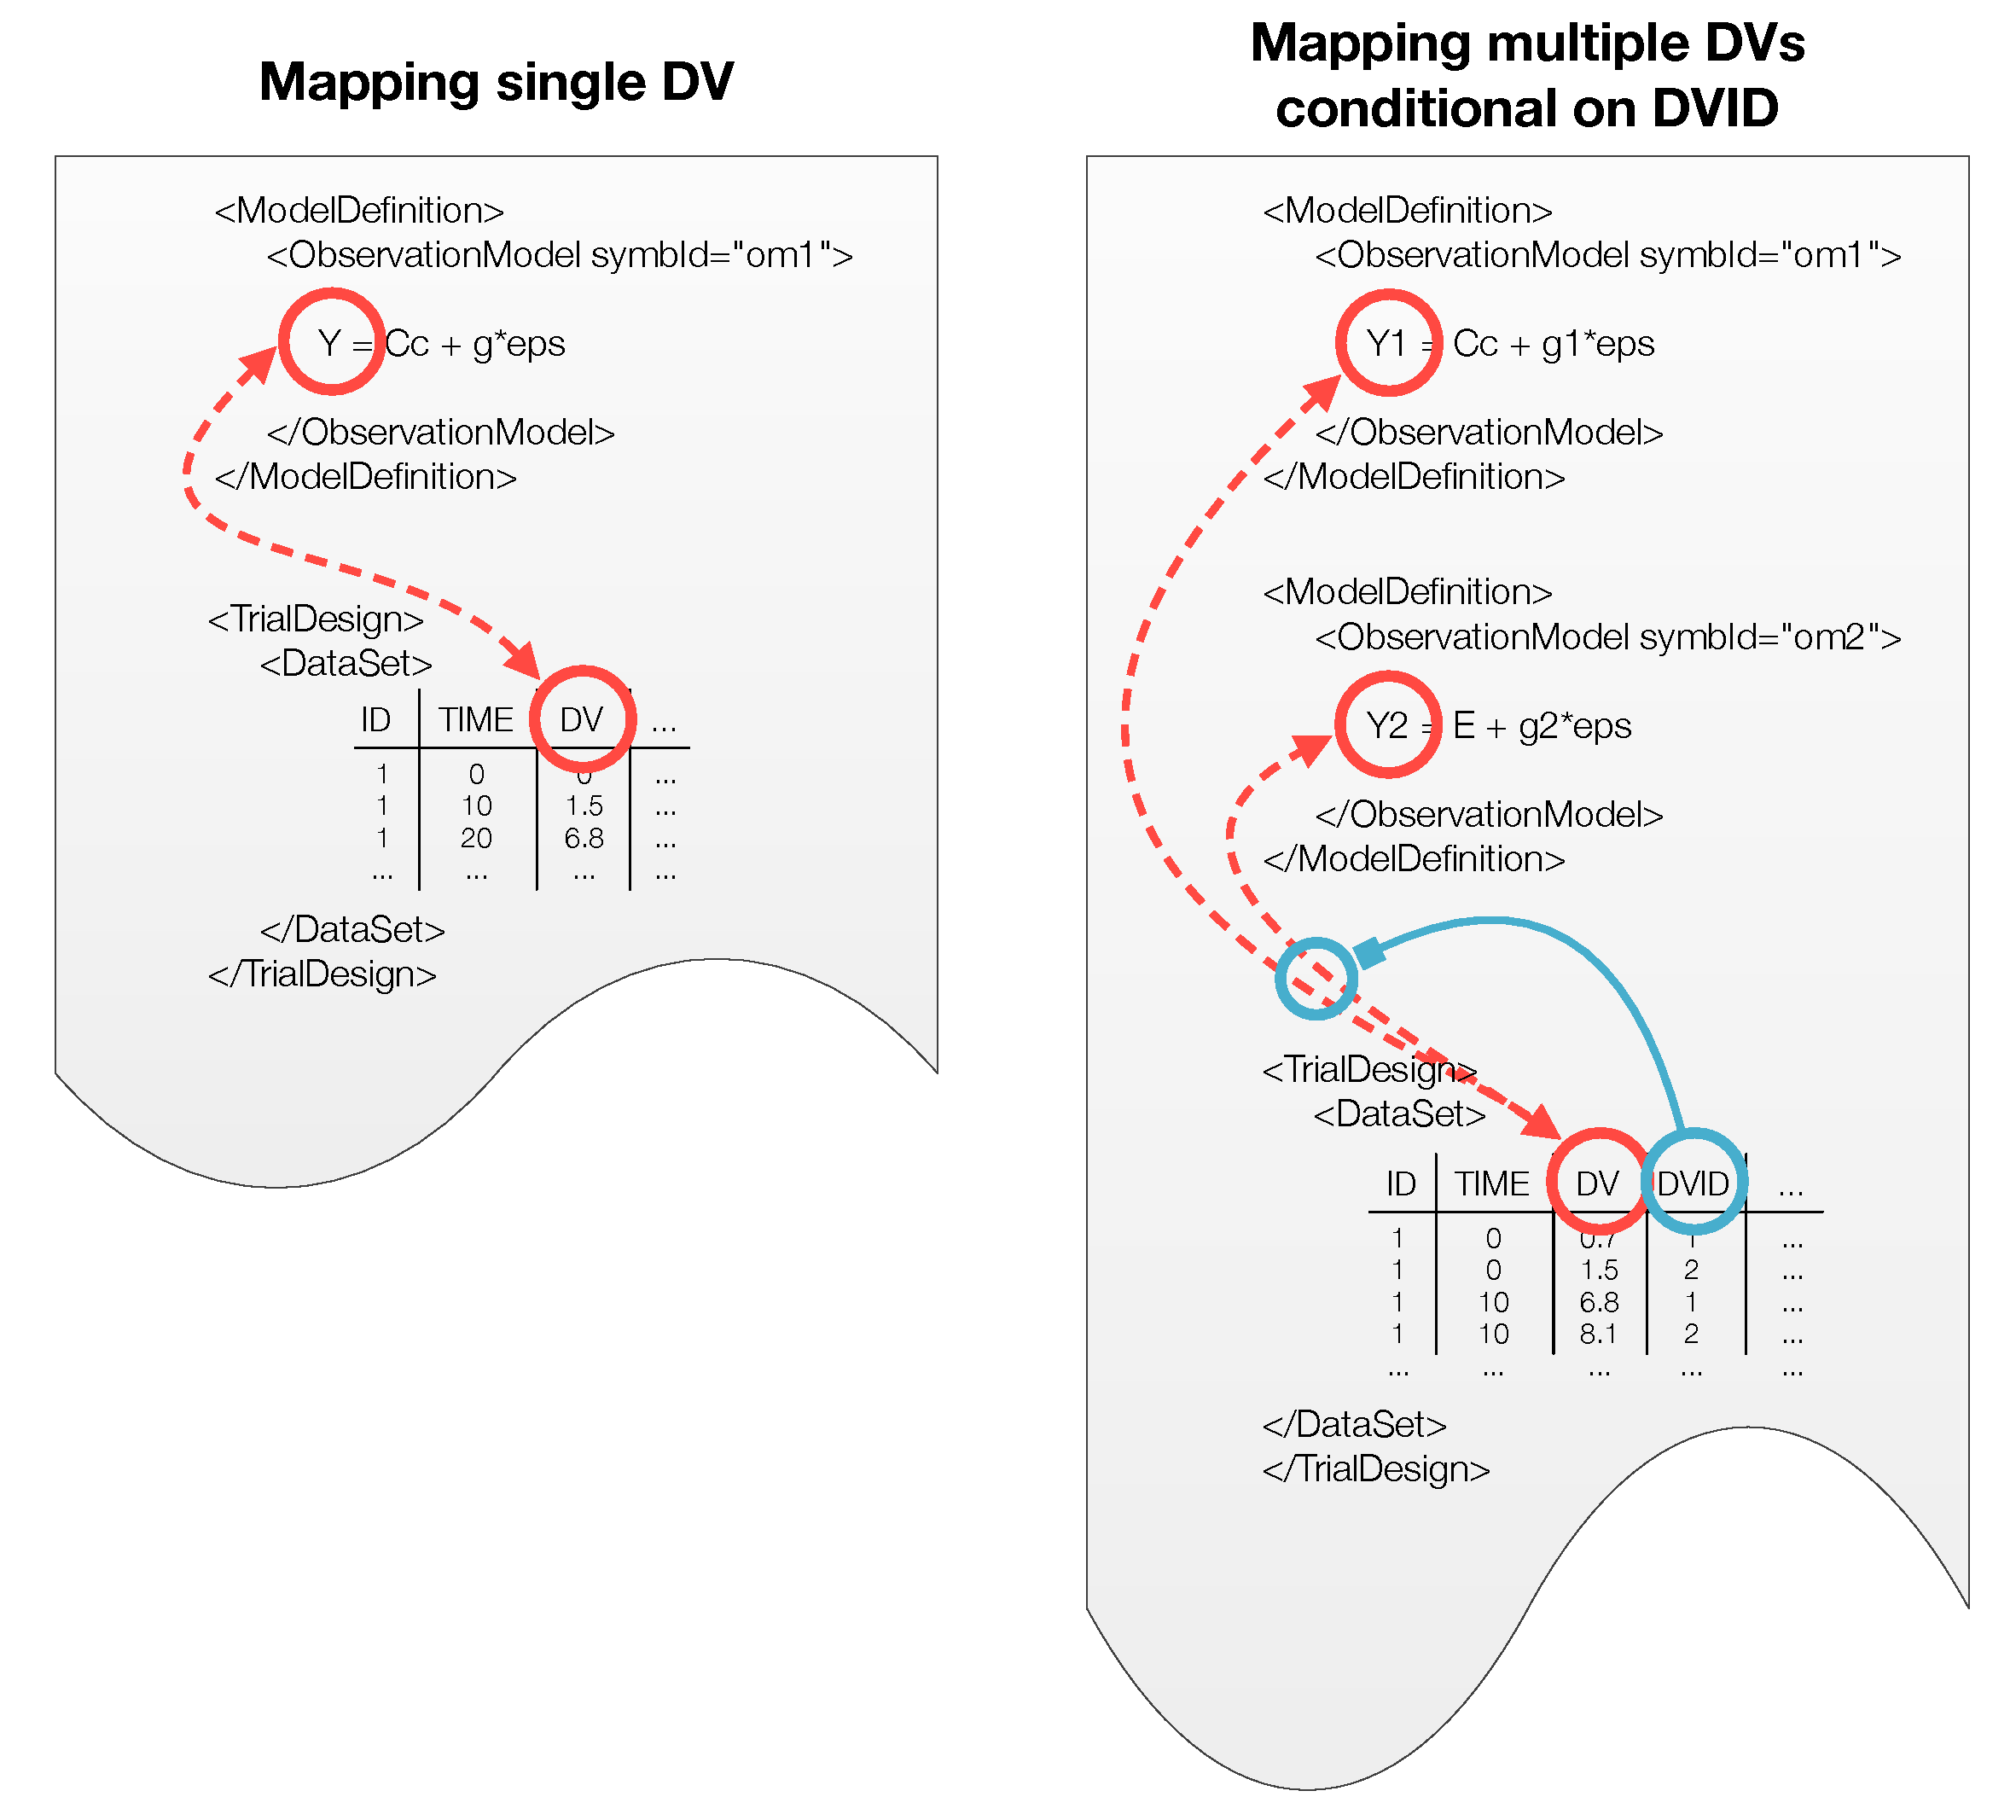
\includegraphics[width=120mm]{pics/mapping1.pdf}
% \caption{....}
% \label{fig:mappingDV}
%\end{figure}


\section{Markov models}
\label{sec:markovModels}
Stimulated by the discussion on the DDMoRE forum, a number of Markov models
was considered. The description and implementation details are given in the following 
sections. 

\subsection{Example 1 -- Simple Markov Model}
\label{subsec:exp1}

\subsection*{Model definition}
\subsubsection*{Observation model}

\begin{itemize}
\item
Type of observed variable -- discrete / categorical
\item
Category variable: $Y$
\item
Initial state variable: $Y_{init}$
\item
Set of categories: $\{\mbox{Alive}, \mbox{Dead}\}$
\item
Transition probability
\begin{align}
& P(\mbox{Alive} \rightarrow \mbox{Dead}) = 0.05 \nonumber
\end{align}
\end{itemize}

\subsection*{Trial Design}

\begin{itemize}
\item
Observations: Y at t=1,...,10.
\end{itemize}


\subsection*{Modelling steps}

\begin{itemize}
\item
Initial states
\begin{align}
& Y_{init} = \left( \begin{array}{c} 100 \\ 0 \end{array} \right) \nonumber
\end{align}
\end{itemize}


\subsection*{PharmML implementation}

\lstset{language=XML}
\begin{lstlisting}
    <ModelDefinition>
        <!-- OBSERVATIONS -->
        <ObservationModel blkId="om1">
            <Discrete>
                <CategoricalData>
                    
                    <ListOfCategories> 
                        <Category symbId="Alive"/>
                        <Category symbId="Dead"/>
                    </ListOfCategories>
                    
                    <CategoryVariable symbId="Y"/>

		    <!-- 100 people - see ModellingSteps/SimulationStep -->
                    <InitialStateVariable symbId="Yinit"/>
                    <PreviousStateVariable symbId="Yp"/>
                    
                    <Dependance type="discreteMarkov"/>
                    
                    <!-- P(Y=Dead|Yp=Alive)=0.05 -->
                    <ProbabilityAssignment>
                        <Probability symbId="p1">
                            <CurrentState>
                                <math:LogicBinop op="eq">
                                    <ct:SymbRef symbIdRef="Y"/>
                                    <ct:SymbRef symbIdRef="Dead"/>
                                </math:LogicBinop>
                            </CurrentState>
                            <PreviousState>
                                <math:LogicBinop op="eq">
                                    <ct:SymbRef symbIdRef="Yp"/>
                                    <ct:SymbRef symbIdRef="Alive"/>
                                </math:LogicBinop>
                            </PreviousState>
                        </Probability>
                        <ct:Assign>
                            <ct:Real>0.05</ct:Real>
                        </ct:Assign>
                    </ProbabilityAssignment>
                    
                </CategoricalData>
            </Discrete>
        </ObservationModel>
    </ModelDefinition>
\end{lstlisting}
Trial design: output of variable $Y$ at t=1,...,10.
\lstset{language=XML}
\begin{lstlisting}
    <TrialDesign>
        <Observations>
            <Observation oid="obsOid">
                <ObservationTimes>
                    <ct:Assign>
                        <ct:Sequence>
                            <ct:Begin><ct:Real>1</ct:Real></ct:Begin>
                            <ct:StepSize><ct:Real>1</ct:Real></ct:StepSize>
                            <ct:End><ct:Real>10</ct:Real></ct:End>
                        </ct:Sequence>
                    </ct:Assign>
                </ObservationTimes>
                <Discrete>
                    <ct:SymbRef blkIdRef="om1" symbIdRef="Y"/>
                </Discrete>
            </Observation>
        </Observations>
    </TrialDesign>
\end{lstlisting}
Modelling step definition and initial assignments, $Y_{init} = (100, 0)$
\lstset{language=XML}
\begin{lstlisting}
    <mstep:ModellingSteps>
        <mstep:SimulationStep oid="simOid">
            
            <mstep:ObservationsReference>
                <ct:OidRef oidRef="obsOid"/>
            </mstep:ObservationsReference>
            
            <ct:VariableAssignment>
                <ct:SymbRef blkIdRef="om1" symbIdRef="Yinit"/>
                <ct:Assign>
                    <ct:Vector>
                        <ct:VectorElements>
                            <ct:Real>100</ct:Real>
                            <ct:Real>0</ct:Real>
                        </ct:VectorElements>
                    </ct:Vector>
                </ct:Assign>
            </ct:VariableAssignment>
\end{lstlisting}



\subsection{Example 2 -- Three State Markov Model}
\label{subsec:exp2}

The next example is build around a Markov chain for three states/categories
which is shown in the figure \ref{fig:example2} and expressed by a set
of pair-wise transition probabilities or a so-called \textbf{left} transition 
(aka stochastic) matrix, on the right in the figure.
\begin{figure}[ht!]
\centering
  \includegraphics[width=120mm]{pics/example2.pdf}
 \caption{Example 2 can be expressed by the basic Markov chain with the
 transition probabilities given below or the transition matrix (right).}
 \label{fig:example2}
\end{figure}


\subsection*{Model definition}
\subsubsection*{Observation model}

\begin{itemize}
\item
Type of observed variable -- discrete / categorical
\item
Category variable: $Y$
\item
Initial state variable: $Y_{init}$
\item
Set of categories: $\{\mbox{Healthy}, \mbox{Sick}, \mbox{Dead}\}$
\item
Transition probabilities
\begin{itemize}
\item
as pairwise conditional transition probabilities
\begin{align}
& P(\mbox{Healthy} \rightarrow \mbox{Dead}) = 0.1 \nonumber \\
& P(\mbox{Healthy} \rightarrow \mbox{Sick}) = 0.2 \nonumber \\
& P(\mbox{Sick} \rightarrow \mbox{Healthy}) = 0.1 \nonumber \\
& P(\mbox{Sick} \rightarrow \mbox{Dead}) = 0.3 \nonumber
\end{align}
\item
or as transition (aka stochastic) matrix
%\[
%\begin{bmatrix}
%    1-0.2-0.1 & 0.2 & 0.01  \\
%    0.1 & 1-0.1-0.3 & 0.03  \\
%    0 & 0 & 1  \\
%\end{bmatrix}
%\]
\[
\begin{blockarray}{cccc}
& H & S & D \\
\begin{block}{c[ccc]}
H &    1-0.2-0.1 & 0.2 & 0.1  \\
S &    0.1 & 1-0.1-0.3 & 0.3  \\
D &    0 & 0 & 1  \\
\end{block}
\end{blockarray}
\]

\end{itemize}
\end{itemize}


\subsection*{Trial Design}

\begin{itemize}
\item
Observations: Y at t=1,...,10.
\end{itemize}


\subsection*{Modelling steps}

\begin{itemize}
\item
Initial states
\begin{align}
& Y_{init} = \left( \begin{array}{c} 100 \\ 0 \\ 0 \end{array} \right) \nonumber
\end{align}
\end{itemize}



\subsection*{PharmML implementation}
The model is a straightforward extension of example 1 for three categories and should
not be shown here except the transition matrix which can be used instead of
the transition probabilities 
\lstset{language=XML}
\begin{lstlisting}
<TransitionMatrix>
    <ct:Matrix matrixType="Any">
        <ct:ColumnNames>
            <ct:SymbRef symbIdRef="Healthy"/>
            <ct:SymbRef symbIdRef="Sick"/>
            <ct:SymbRef symbIdRef="Dead"/>
        </ct:ColumnNames>
        <ct:MatrixRow>
            <ct:Real>0.7</ct:Real><ct:Real>0.2</ct:Real><ct:Real>0.1</ct:Real>
        </ct:MatrixRow>
        <ct:MatrixRow>
            <ct:Real>0.1</ct:Real><ct:Real>0.6</ct:Real><ct:Real>0.3</ct:Real>
        </ct:MatrixRow>
        <ct:MatrixRow>
            <ct:Real>0</ct:Real><ct:Real>0</ct:Real><ct:Real>0.1</ct:Real>
        </ct:MatrixRow>
    </ct:Matrix>
</TransitionMatrix>
\end{lstlisting}


\subsection{Example 3 -- Stratified Markov Model}
\label{subsec:exp3}

The transition probabilities vary now conditional on the sex of 
the subjects. For example the probability for a healthy female to 
get sick is lower, 0.1, then for a male, 0.2. See Figure \ref{fig:markovMatrixCond}
for the Markov chain network and transition matrix for this model.

\begin{figure}[ht!]
\centering
  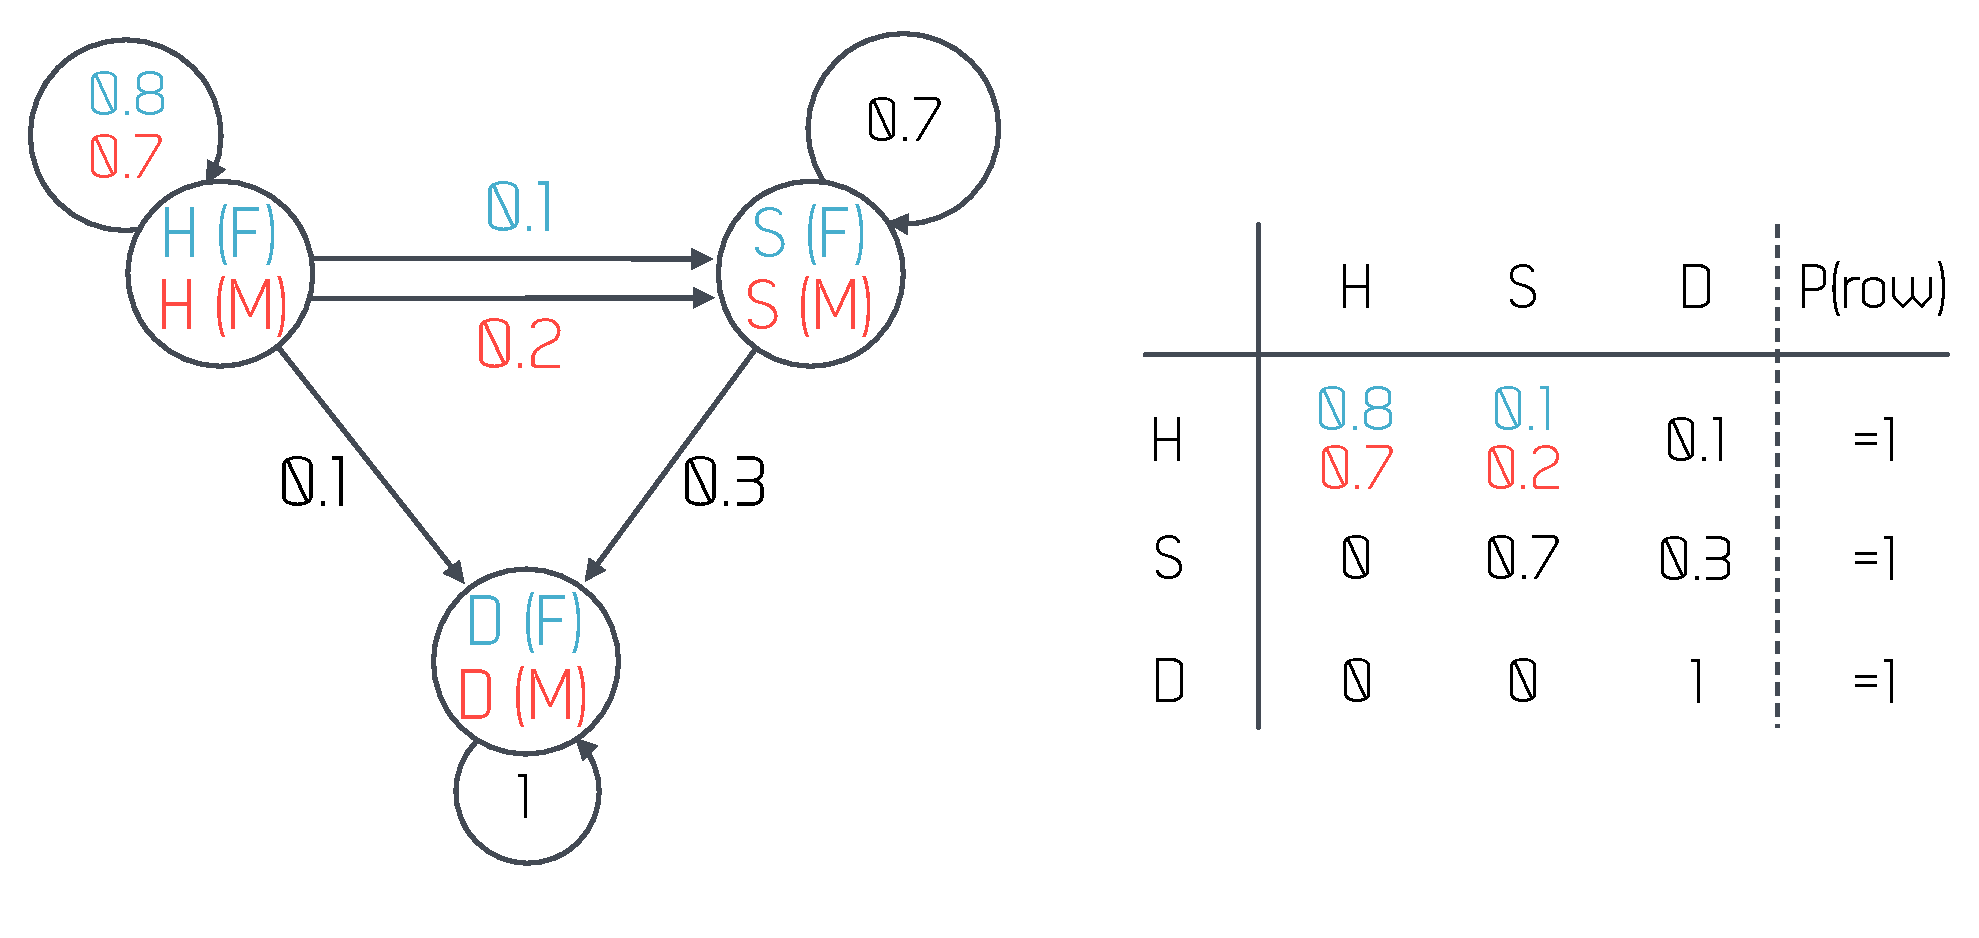
\includegraphics[width=120mm]{pics/markovMatrixCond.pdf}
 \caption{Example 3 -- a transition matrix defined conditional on sex of the subjects.}
 \label{fig:markovMatrixCond}
\end{figure}

\subsection*{Model definition}

\subsubsection*{Covariate model}
\begin{itemize}
\item
Age -- continuous covariate
\item
Sex = \{F, M\} -- categorical covariate
\end{itemize}

\subsubsection*{Observation model}

\begin{itemize}
\item
Type of observed variable -- discrete / categorical
\item
Category variable: $Y$
\item
Initial state variable: $Y_{init}$
\item
Set of categories: $\{\mbox{Healthy}, \mbox{Sick}, \mbox{Dead}\}$
\item
Transition probabilities
\begin{itemize}
\item
as pairwise conditional transition probabilities
\begin{align}
& P(\mbox{Healthy} \rightarrow \mbox{Sick} | \; SEX==F) = 0.1 \nonumber \\
& P(\mbox{Healthy} \rightarrow \mbox{Sick} | \; SEX==M) = 0.2 \nonumber \\
& P(\mbox{Sick} \rightarrow \mbox{Healthy}) = 0.1 \nonumber \\
& P(\mbox{Sick} \rightarrow \mbox{Dead}) = 0.3 \nonumber \\
& \mbox{other probabilities follow from the property 'left stochastic matrix'} \nonumber
\end{align}
\item
or as transition (aka stochastic) matrix
\[
\begin{blockarray}{cccc}
& H & S & D \\
\begin{block}{c[ccc]}
H &	0.7 & \left\{\begin{array}{ll}
      	0.1 & SEX== F \\
      	0.2 & SEX== M \\
\end{array}\right. & 0.1  \\\\
S &    0.1 & 0.6 & 0.3  \\\\
D &    0 & 0 & 1  \\
\end{block}
\end{blockarray}
\]
\end{itemize}
\end{itemize}

\subsection*{Trial Design}

\begin{itemize}
\item
Observations: Y at t=1,...,10.
\end{itemize}

\subsection*{Modelling steps}

\begin{itemize}
\item
Initial states
\begin{align}
& Y_{init} = \left( \begin{array}{c} 100 \\ 0 \\ 0 \end{array} \right) \nonumber
\end{align}
\end{itemize}

\subsection*{PharmML implementation}
Most of the model elements is identical to that of example in section \ref{subsec:exp2}
except the conditional transition probabilities, which XML encoding will be shown
here only.  The probabilities can be expresses pairwise or a transition matrix as the following 
code snippet show.

\begin{itemize}
\item
Pairwise probabilities (only the conditional ones are shown for brevity)

\lstset{language=XML}
\begin{lstlisting}
        <!-- P(Yp=Healthy -> Y=Sick | SEX=F)=0.1 -->
        <ProbabilityAssignment>
            <Probability>
                <CurrentState>
                    <math:LogicBinop op="eq">
                        <ct:SymbRef symbIdRef="Y"/>
                        <ct:SymbRef symbIdRef="Dead"/>
                    </math:LogicBinop>
                </CurrentState>
                <PreviousState>
                    <math:LogicBinop op="eq">
                        <ct:SymbRef symbIdRef="Yp"/>
                        <ct:SymbRef symbIdRef="Sick"/>
                    </math:LogicBinop>
                </PreviousState>
                <Condition>
                    <math:LogicBinop op="eq">
                        <ct:SymbRef symbIdRef="SEX"/>
                        <ct:CatRef catIdRef="F"/>
                    </math:LogicBinop>
                </Condition>
            </Probability>
            <ct:Assign>
                <ct:Real>0.1</ct:Real>
            </ct:Assign>
        </ProbabilityAssignment>
        
        <!-- P(Yp=Healthy -> Y=Sick | SEX=M)=0.1 -->
        <ProbabilityAssignment>
            <Probability>
                <CurrentState>
                    <math:LogicBinop op="eq">
                        <ct:SymbRef symbIdRef="Y"/>
                        <ct:SymbRef symbIdRef="Sick"/>
                    </math:LogicBinop>
                </CurrentState>
                <PreviousState>
                    <math:LogicBinop op="eq">
                        <ct:SymbRef symbIdRef="Yp"/>
                        <ct:SymbRef symbIdRef="Healthy"/>
                    </math:LogicBinop>
                </PreviousState>
                <Condition>
                    <math:LogicBinop op="eq">
                        <ct:SymbRef symbIdRef="SEX"/>
                        <ct:CatRef catIdRef="M"/>
                    </math:LogicBinop>
                </Condition>
            </Probability>
            <ct:Assign>
                <ct:Real>0.2</ct:Real>
            </ct:Assign>
        </ProbabilityAssignment>
\end{lstlisting}

\item
Transition matrix -- we use the fact that a matrix element can contain an arbitrary expression,
also a piecewise function used here for the transition probability from the \emph{Healthy} to 
\emph{Sick} state conditioned on the covariate \emph{Sex}. 
\lstset{language=XML}
\begin{lstlisting}
        <TransitionMatrix symbId="T1">
            <ct:Matrix matrixType="Any">
                <ct:ColumnNames>
                    <ct:SymbRef symbIdRef="Healthy"/>
                    <ct:SymbRef symbIdRef="Sick"/>
                    <ct:SymbRef symbIdRef="Dead"/>
                </ct:ColumnNames>
                <ct:MatrixRow>
                    <ct:Real>0.7</ct:Real>
                    <ct:Assign>
                        <ct:Piecewise>
                            <math:Piece>
                                <ct:Real>0.8</ct:Real>
                                <math:Condition>
                                    <math:LogicBinop op="eq">
                                        <ct:SymbRef symbIdRef="Sex"/>
                                        <ct:CatRef catIdRef="F"/>
                                    </math:LogicBinop>
                                </math:Condition>
                            </math:Piece>
                            <math:Piece>
                                <ct:Real>0.7</ct:Real>
                                <math:Condition>
                                    <math:LogicBinop op="eq">
                                        <ct:SymbRef symbIdRef="Sex"/>
                                        <ct:CatRef catIdRef="M"/>
                                    </math:LogicBinop>
                                </math:Condition>
                            </math:Piece>
                        </ct:Piecewise>
                    </ct:Assign>
                    <ct:Real>0.1</ct:Real>
                </ct:MatrixRow>
                <ct:MatrixRow>
                    <ct:Real>0.1</ct:Real><ct:Real>0.6</ct:Real><ct:Real>0.3</ct:Real>
                </ct:MatrixRow>
                <ct:MatrixRow>
                    <ct:Real>0</ct:Real><ct:Real>0</ct:Real><ct:Real>0.1</ct:Real>
                </ct:MatrixRow>
            </ct:Matrix>
        </TransitionMatrix>
\end{lstlisting}
\end{itemize}
Note, that the order of probabilities is defined by the order of categories/states names in the \xelem{ColumnNames}.
Because the transition matrix is symmetric specifying only the column names is sufficient. 

\subsection{Example 4 -- Micro Simulation Model}
\label{subsec:exp4}

\subsection*{Model definition}

\subsubsection*{Covariate model}
\begin{itemize}
\item
Age -- continuous covariate
\item
Sex = \{F, M\} -- categorical covariate
\end{itemize}
Individual covariates are stored in the trial design, see below.

\subsubsection*{Observation model}

\begin{itemize}
\item
Type of observed variable -- discrete / categorical
\item
Category variable: $Y$
\item
Initial state variable: $Y_{init}$
\item
Set of categories: $\{\mbox{Healthy}, \mbox{Sick}, \mbox{Dead}\}$
\item
Transition probabilities
\begin{itemize}
\item
as pairwise conditional transition probabilities
%
%Healthy to Dead: Age/1000\\
%Healthy to Sick: 0.1* (1 + Male) + 0.01*Age and never more than 0.8\\
%Sick to Healthy 0.1\\
%Sick to Dead:  0.01*Age+0.2*Male and never more than 0.9
\begin{align}
& P(\mbox{Healthy} \rightarrow \mbox{Dead}) = \mbox{Age}/100 \nonumber \\
p_{HS} := \quad & P(\mbox{Healthy} \rightarrow \mbox{Sick} | \; p_{HS} < 0.8) = 0.1(1 + \mbox{Male}) + 0.01\times\mbox{Age} \nonumber \\
& P(\mbox{Sick} \rightarrow \mbox{Healthy}) = 0.1 \nonumber \\
p_{SD} := \quad & P(\mbox{Sick} \rightarrow \mbox{Dead} | \; p_{SD} < 0.9) = 0.01\times\mbox{Age}+0.2\times\mbox{Male} \nonumber
\end{align}
\item
Transition matrix becomes complex with the additional boundaries
on the probabilities and it's probably a better to encode it pairwise
as above.
%\[
%T1 = 
%\begin{blockarray}{cccc}
%& \mbox{H} & \mbox{S} & \mbox{D} \\
%\begin{block}{c[ccc]}
%\mbox{H} & 0.7 	& 0.1(1 + \mbox{Male}) + 0.01\times\mbox{Age } \& \;p_{HS} < 0.8 & 0.1  \\\\
%\mbox{S} 	& 0.1 	& 0.6 & 0.01\times\mbox{Age}+0.2\times\mbox{Male } \& \;p_{SD} < 0.9  \\\\
%\mbox{D} 	& 0 		& 0 & 1  \\
%\end{block}
%\end{blockarray}
%%
%%\begin{bmatrix}
%%    0.7 & 0.2 & 0.01  \\
%%    0.1 & 0.6 & 0.03  \\
%%    0 & 0 & 1  \\
%%\end{bmatrix}
%\]
\end{itemize}
\end{itemize}



\subsection*{Trial Design}

\begin{itemize}
\item
Observations: Y at t=1,...,10.
\item
Covariates
\begin{itemize}
\item
continuous: Age = 1, 2, 3, 4, ..., 100

\item
categorical: Sex = \{F, M\} with Male = 0,1,0,1 .... (100 times)
\end{itemize}
\end{itemize}



\subsection*{Modelling steps}

\begin{itemize}
\item
Initial states
\begin{align}
& Y_{init} = \left( \begin{array}{c} 100 \\ 0 \\ 0 \end{array} \right) \nonumber
\end{align}
\end{itemize}

\subsection*{PharmML implementation}
The covariates are coming here as individual values, meaning that they
have to be provided as a table. This is when the \xelem{TrialDesign} is
very helpful as it is equipped with the required structure.
It is sufficient to declare the covariates in the \xelem{CovariateModel} within 
\xelem{ModelDefinition} as the following snippet shows
\lstset{language=XML}
\begin{lstlisting}
        <CovariateModel blkId="cm1">
            <Covariate symbId="AGE">
                <Continuous/>
            </Covariate>
            
            <Covariate symbId="MALE">
                <Categorical>
                    <Category catId="F"/>
                    <Category catId="M"/>
                </Categorical>
            </Covariate>
        </CovariateModel>
\end{lstlisting}
the proper values are stored then in the \xelem{IndividualCovariates} in 
\xelem{TrialDesign}
\lstset{language=XML}
\begin{lstlisting}
        <Covariates>
            <!--    Male = 0,1,0,1 .... (100 times)
                    Age = 1,2,3,4,...100-->
            <IndividualCovariates>
                <ColumnMapping>
                    <ds:ColumnRef columnIdRef="SEX"/>
                    <ct:SymbRef blkIdRef="cm1" symbIdRef="Sex"/>
                    <ds:CategoryMapping>
                        <ds:Map dataSymbol="1" modelSymbol="F"/>
                        <ds:Map dataSymbol="0" modelSymbol="M"/>
                    </ds:CategoryMapping>
                </ColumnMapping>
                <ColumnMapping>
                    <ds:ColumnRef columnIdRef="AGE"/>
                    <ct:SymbRef blkIdRef="cm1" symbIdRef="Age"/>
                </ColumnMapping>
                <ds:DataSet>
                    <ds:Definition>
                        <ds:Column columnId="ID" columnType="id" valueType="id" columnNum="1"/>
                        <ds:Column columnId="SEX" columnType="covariate" valueType="real" columnNum="2"/>
                        <ds:Column columnId="AGE" columnType="covariate" valueType="real" columnNum="3"/>
                    </ds:Definition>
                    <ds:Table>
                        <ds:Row>
                            <ct:Id>i1</ct:Id><ct:Real>0</ct:Real><ct:Real>1</ct:Real>
                        </ds:Row>
                        <ds:Row>
                            <ct:Id>i1</ct:Id><ct:Real>1</ct:Real><ct:Real>2</ct:Real>
                        </ds:Row>
                        <ds:Row>
                            <ct:Id>i1</ct:Id><ct:Real>0</ct:Real><ct:Real>3</ct:Real>
                        </ds:Row>
                        <ds:Row>
                            <ct:Id>i1</ct:Id><ct:Real>1</ct:Real><ct:Real>4</ct:Real>
                        </ds:Row>
                        <!-- omitted subjects -->
                        <ds:Row>
                            <ct:Id>i100</ct:Id><ct:Real>1</ct:Real><ct:Real>100</ct:Real>
                        </ds:Row>
                    </ds:Table>
                </ds:DataSet>
            </IndividualCovariates>
        </Covariates>
    </TrialDesign>
\end{lstlisting}
\xelem{ColumnMapping} elements are declared to provide the required information 
how to connect the model and the covariates.

From the model definition we show here only the implementation of one
probability, $P(\mbox{Sick} \rightarrow \mbox{Dead} | \; p_{SD} < 0.9)$, the remaining transition 
probabilities are analog.
\lstset{language=XML}
\begin{lstlisting}
        <!-- Healthy to Sick -->
        <!-- pHS:= P(y=Dead|yp=Healthy & pHS<0.8 = 0.1* (1 + Male) +  0.01*Age -->
        <ProbabilityAssignment>
            <Probability symbId="pHS">
                <CurrentState>
                    <math:LogicBinop op="eq">
                        <ct:SymbRef symbIdRef="y"/>
                        <ct:SymbRef symbIdRef="Sick"/>
                    </math:LogicBinop>
                </CurrentState>
                <PreviousState>
                    <math:LogicBinop op="eq">
                        <ct:SymbRef symbIdRef="yp"/>
                        <ct:SymbRef symbIdRef="Healthy"/>
                    </math:LogicBinop>
                </PreviousState>
                <Condition>
                    <math:LogicBinop op="lt">
                        <ct:SymbRef symbIdRef="pHS"/>
                        <ct:Real>0.8</ct:Real>
                    </math:LogicBinop>
                </Condition>
            </Probability>
            <ct:Assign>
                <math:Binop op="plus">
                    <math:Binop op="times">
                        <ct:Real>0.1</ct:Real>
                        <math:Binop op="plus">
                            <ct:Real>1</ct:Real>
                            <ct:SymbRef symbIdRef="Male"/>
                        </math:Binop>
                    </math:Binop>
                    <math:Binop op="times">
                        <ct:Real>0.01</ct:Real>
                        <ct:SymbRef symbIdRef="Age"/>
                    </math:Binop>
                </math:Binop>
            </ct:Assign>
        </ProbabilityAssignment>
\end{lstlisting}
Note, that the probability is assigned a symbol identifier \xatt{symbId="pHS"}
which is then used to express the condition $p\_{SD}<0.9$

\subsection*{Out of scope}
Compared to the original description not covered is the specification of 
\begin{itemize}
\item 
Simulation execution, here from the original description: \emph{ [...] each time 
step we want Age of each individual to increase by 1 before any transitions 
are executed: Age $\leftarrow$ Age + 1: This is executed for living individuals only}
\item 
Output, here from the original description: \emph{[...] number of people in each 
state each year total and stratified by age groups above and below 50, and Male.} \\
Such analysis is assumed to be carried out by a downstream tool as it was 
not in the scope and requirements for PharmML.
\end{itemize}


%\section{Multiple infusions}
%
%Alternatively, you could use DesignParameter to encode the 
%amount vector
%\lstset{language=XML}
%\begin{lstlisting}
%		<mdef:DesignParameter symbId="doseAmountVector">
%			<ct:Assign>
%				<ct:Vector>
%					<ct:VectorElements>
%						<ct:Real>1</ct:Real>
%						<ct:Real>2</ct:Real>
%						<ct:Real>1</ct:Real>
%						<ct:Real>5</ct:Real>
%						<!-- ... -->
%					</ct:VectorElements>
%				</ct:Vector>
%			</ct:Assign>
%		</mdef:DesignParameter>
%\end{lstlisting}
%
%and then refer to it in (see in bold below)
%\lstset{language=XML}
%\begin{lstlisting}
%	<Interventions>
%		<Administration oid="inf1">
%			<Infusion>
%				<DoseAmount>
%					<ct:SymbRef symbIdRef="Ad"/>
%					<ct:Assign>
%						<math:Binop op="divide">
%							<math:Binop op="times">
%								<ct:SymbRef symbIdRef="doseAmountVector"/>
%								<ct:SymbRef blkIdRef="mmcvt" symbIdRef="wgt" />
%							</math:Binop>
%							<ct:SymbRef blkIdRef="mmpar" symbIdRef="V" />
%						</math:Binop>
%					</ct:Assign>
%				</DoseAmount>
%				<DosingTimes>
%					<ct:Assign>
%						<ct:Vector>
%							<ct:VectorElements>
%								<ct:Real>0</ct:Real>
%								<ct:Real>5</ct:Real>
%								<ct:Real>10</ct:Real>
%								<!-- ... -->
%							</ct:VectorElements>
%						</ct:Vector>
%					</ct:Assign>
%				</DosingTimes>
%				<Rate>
%					<ct:Assign>
%						<ct:Vector>
%							<ct:VectorElements>
%								<ct:Real>10</ct:Real>
%								<ct:Real>15</ct:Real>
%								<ct:Real>20</ct:Real>
%								<!-- ... -->
%							</ct:VectorElements>
%						</ct:Vector>	
%					</ct:Assign>
%				</Rate>
%				ALTERNATIVE 
%				<Duration>
%					<ct:Assign>
%						<ct:Vector>
%							<ct:VectorElements>
%								<ct:Real>10</ct:Real>
%								<ct:Real>15</ct:Real>
%								<ct:Real>20</ct:Real>
%								<!-- ... -->
%							</ct:VectorElements>
%						</ct:Vector>
%					</ct:Assign>
%				</Duration>
%			</Infusion>
%		</Administration>
%\end{lstlisting}
%


















\appendix


%\paragraph{Covariate model}
%Covariate model is barely covered so far. See also \cite{Keizer:2011aa}. Missing are following features:\\
%For categorical covariates:\\
%-- categorical distribution of categorical covariates \\
%---- estimating categorical distribution from external data file -- TEST \\
%---- sampling from known categorical distribution -- TEST \\
%---- clusters of categorical covariates \\
%For continuous covariates:\\
%-- power-normal distribution for continuous covariates \\
%---- estimating parameters $\lambda$,$\mu$,$\sigma$ from external data file \\
%---- sampling from known power-normal distribution \\
%---- conditional distribution of continuous covariates - DONE \\
%---- selecting criteria for continuous covariates \\
%---- dependent distribution of continuous covariates \\
%---- correlated continuous covariates \\
%For both types: \\
%-- selection/exclusion criteria missing \\


%\bibliographystyle{plain}
\bibliographystyle{apalike}
\bibliography{pharmml-specification}
\end{document}

